%%%%%%%%%%%%%%%%%%%%%%%%%%%%%%%%%%%%%%%%%%%%%%%%%%%%%%%%%%%%%%%%%%%%%
%% This is a "template" model document for submission to the
%% American Chemical Society (ACS).
%%
%% The guidance here contains information about how you may wish to
%% modify it to match the requirements of various ACS journals. The
%% ACS do *not* typeset accepted articles using LaTeX, so there is
%% no specific class required.
%%
%% This template deliberately does *not* seek to reproduce
%% the layout of the typeset journal: this is explicitly not
%% required by the ACS for LaTeX submissions.
%%
%% Please report any issues with the template at
%% https://github.com/josephwright/acs-template/issues
%%
%% Released under the Creative Commons 0 license
%% https://creativecommons.org/public-domain/cc0/
%% 
%% Copyight (c) 2025 Joseph Wright
%%%%%%%%%%%%%%%%%%%%%%%%%%%%%%%%%%%%%%%%%%%%%%%%%%%%%%%%%%%%%%%%%%%%%
\documentclass[letterpaper]{article}

%%%%%%%%%%%%%%%%%%%%%%%%%%%%%%%%%%%%%%%%%%%%%%%%%%%%%%%%%%%%%%%%%%%%%
%% Font setup - delete if you are using LuaLaTeX
%%%%%%%%%%%%%%%%%%%%%%%%%%%%%%%%%%%%%%%%%%%%%%%%%%%%%%%%%%%%%%%%%%%%%
\usepackage[T1]{fontenc}

%%%%%%%%%%%%%%%%%%%%%%%%%%%%%%%%%%%%%%%%%%%%%%%%%%%%%%%%%%%%%%%%%%%%%
%% Adjust the margins and allow for line spacing
%%%%%%%%%%%%%%%%%%%%%%%%%%%%%%%%%%%%%%%%%%%%%%%%%%%%%%%%%%%%%%%%%%%%%
\usepackage{geometry}
\geometry{margin = 1in}
\usepackage{setspace}

%%%%%%%%%%%%%%%%%%%%%%%%%%%%%%%%%%%%%%%%%%%%%%%%%%%%%%%%%%%%%%%%%%%%%
%% Reference support
%%
%% The recommended method for producing the reference section is
%% to use biblatex. If you wish to use a classical BibTeX
%% approach, this is easiest to achieve using the achemso package.
%% In that case, you should remove the biblatex lines.
%%%%%%%%%%%%%%%%%%%%%%%%%%%%%%%%%%%%%%%%%%%%%%%%%%%%%%%%%%%%%%%%%%%%%
% You can adjust the printing of DOI, article title, etc. using
% package options, e.g. "doi = true"; see the biblatex manual for
% details of adjusting the number of authors printed, e.g.
% "maxnames = 15" to print no more than 15 authors.
\usepackage[style = chem-acs,articletitle=true]{biblatex}
\addbibresource{reference.bib}
% If you are using classical BibTeX, remove the above lines and 
% uncomment:
%\usepackage{achemso}

%%%%%%%%%%%%%%%%%%%%%%%%%%%%%%%%%%%%%%%%%%%%%%%%%%%%%%%%%%%%%%%%%%%%%
%% Graphic inclusion and scheme and chart support
%%%%%%%%%%%%%%%%%%%%%%%%%%%%%%%%%%%%%%%%%%%%%%%%%%%%%%%%%%%%%%%%%%%%%
\usepackage{graphicx}
\usepackage{float}
\newfloat{scheme}{htbp}{los}
\floatname{scheme}{Scheme}
\floatname{chart}{Chart}
\newfloat{graph}{htbp}{loh}
\usepackage{caption}
\usepackage{amsmath}
\usepackage{amssymb}
\usepackage[none]{hyphenat}
\usepackage{enumitem}
\usepackage{tikz}
\usepackage{dblfloatfix}
\usepackage{lipsum}
\usepackage{multicol}
\usepackage{float}
\usepackage[table]{xcolor}
\usepackage{tikz}
\usetikzlibrary{arrows.meta, positioning}
\usepackage{booktabs}
\usepackage{mdframed}
\usepackage{placeins}
\usepackage{etoolbox}
\usepackage{multirow}
\usepackage{stfloats}
\usepackage[ruled]{algorithm2e}

%%%%%%%%%%%%%%%%%%%%%%%%%%%%%%%%%%%%%%%%%%%%%%%%%%%%%%%%%%%%%%%%%%%%%
%% Common support packages
%%%%%%%%%%%%%%%%%%%%%%%%%%%%%%%%%%%%%%%%%%%%%%%%%%%%%%%%%%%%%%%%%%%%%
\usepackage{chemformula} % Formulas using \ch{}
% or
\usepackage[version = 4]{mhchem} % Formulas using \ce{}

%%%%%%%%%%%%%%%%%%%%%%%%%%%%%%%%%%%%%%%%%%%%%%%%%%%%%%%%%%%%%%%%%%%%%
%% Many journals require that sections are unnumbered: this 
%% is activated here
%%%%%%%%%%%%%%%%%%%%%%%%%%%%%%%%%%%%%%%%%%%%%%%%%%%%%%%%%%%%%%%%%%%%%
\setcounter{secnumdepth}{-1}

%%%%%%%%%%%%%%%%%%%%%%%%%%%%%%%%%%%%%%%%%%%%%%%%%%%%%%%%%%%%%%%%%%%%%
%% Place any additional macros here.  Please use \newcommand* where
%% possible, and avoid layout-changing macros (which are not used
%% when typesetting).
%%%%%%%%%%%%%%%%%%%%%%%%%%%%%%%%%%%%%%%%%%%%%%%%%%%%%%%%%%%%%%%%%%%%%
\newcommand*\mycommand[1]{\texttt{\emph{#1}}}

%%%%%%%%%%%%%%%%%%%%%%%%%%%%%%%%%%%%%%%%%%%%%%%%%%%%%%%%%%%%%%%%%%%%%
%% Author and title data:
%% the authblk package is currently the simplest way to provide this
%%%%%%%%%%%%%%%%%%%%%%%%%%%%%%%%%%%%%%%%%%%%%%%%%%%%%%%%%%%%%%%%%%%%%
\usepackage{authblk}
\author[1]{Yamini Chitikela}
\author[2]{Zhenquan Jia*}
\author[1]{Chunjiang Zhu*}
\affil[1]{Department of Computer Science, Old Dominion University}
\affil[2]{Department of Biology, University of North Carolina at Greensboro}

\title{A Graph-based QSAR Modeling Pipeline for Predicting In vitro PubChem Assays and In vivo Human hepatotoxicity: Mechanistic Analysis of Caspase-3/7 Activation}
% Use the \date command for email address(s) of corresponding authors
\date{*Email: z\_jia@uncg.edu, czhu@odu.edu}

\begin{document}

\maketitle

\newpage

% \begin{abstract}
% \textbf{Background:} 
% Caspase-3 and -7 are key effector caspases in the apoptotic pathway, a form of programmed cell death, and their activities serve as a well-established biomarker for evaluating environmental chemical toxicity and informing chemical risk assessment. Loss of mitochondrial membrane potential is a key event in the activation of Caspase-3/7 signaling and the subsequent induction of apoptosis. Therefore, \emph{simultaneous} assessment of mitochondrial membrane potential and Caspase-3/7 activity enables elucidation of the mechanisms and pathways through which apoptosis is initiated.

% Rapid and accurate assessment of the potential toxicity of environmental chemicals and drugs remains a major challenge. Quantitative Structure–Activity Relationship (QSAR) modeling have been widely used for toxicity prediction. Graph-based approaches encode compounds directly as molecular graphs, allowing structure-activity relationships to be learnt from molecular topology without the information loss in binary fingerprints. While advanced graph models such as graph transformers (GTs) have shown outstanding performance in many domains, they have not been fully leveraged in QSAR modeling on Caspase and mitochondrial toxicity.

% \textbf{Methods:} 
% We propose a QSAR modeling pipeline that encompasses assay data preprocessing, feature representations (fingerprints and molecular graphs), and benchmarking machine learning (ML) models, including classic ML models, graph neural networks (GNNs), GTs, and their consensus ensembles. Based on \emph{in vitro} Caspase and mitochondrial assays in PubChem, we applied the pipeline to predict Caspase-3/7 activation and mitochondrial membrane potential (MMP). Beyond \emph{in vitro} assays, we also built \emph{in vivo} QSAR modeling for FDA-approved Drug-Induced Liver Injury (DILI). Moreover, mechanistic analysis on Caspase-3/7 activation was conducted by comparing with MMP disruption to identify chemical substructures that may be responsible for dual activations. We also investigated \emph{cell-line-specific} responses by identifying structural motifs that selectively induce Caspase-3/7 activation in individual cell lines.

% \textbf{Results:} 
% Experimental evaluations show that GTs and GNNs outperformed classic ML models when the number of active compounds is large, such as MMP disruption, while GTs and classic ML models performed good for highly imbalance data with limited active compounds, such as Caspase-3/7 activation. For DILI prediction, the full consensus model achieved the highest AUC 0.69 and the graph transformer method, Graphormer, had the highest F1 score 0.79, both surpassing the previous best model with AUC 0.63 and F1 0.65 with a large margin.

% Our mechanistic analysis shows that phenolic compounds bearing a  para-hydroxyphenyl motif, as well as members of the lipophilic chain family with long alkyl chains can trigger the collapse of MMP, leading to the activation of Caspases-3 and -7. Human embryonic kidney (HEK293) was the only cell line with a distinct structural motif: 1,1-dichloroethane and chlorobenzene. Human neuroblastoma (SK-N-SH) is uniquely impacted by an epoxide fragment, and rat hepatoma (H-4-II-E) is uniquely impacted by a tetramethylcyclohexene motif and an acetaldehyde fragment.


% \textbf{Conclusions:} 
% Our proposed graph-based QSAR modeling pipeline, including data preprocessing, feature representations, and incorporation of advanced graph deep learning approaches, is highly effective in predicting not only on Caspase-3/7 activation and membrane potential collapse, but also on human hepatotoxicity induced by FDA-approved drugs. As future research directions, we will leverage extra information, e.g., biological activity and findings in existing toxicity literature, and recent advances in large language models and agentic AI to further improve the prediction of FDA-approved DILI and enable a sensitive and specific framework for assessing human hepatotoxicity of environmental compounds.
% \end{abstract}
\clearpage

\begin{center}
    \large \bf For Table of Contents Only
\end{center}

\begin{figure*}[h]
    \centering
    \includegraphics[width=.4\textwidth]{figures/TOC Graphic.png}
\end{figure*}
\begin{figure*}[h]
    \centering
    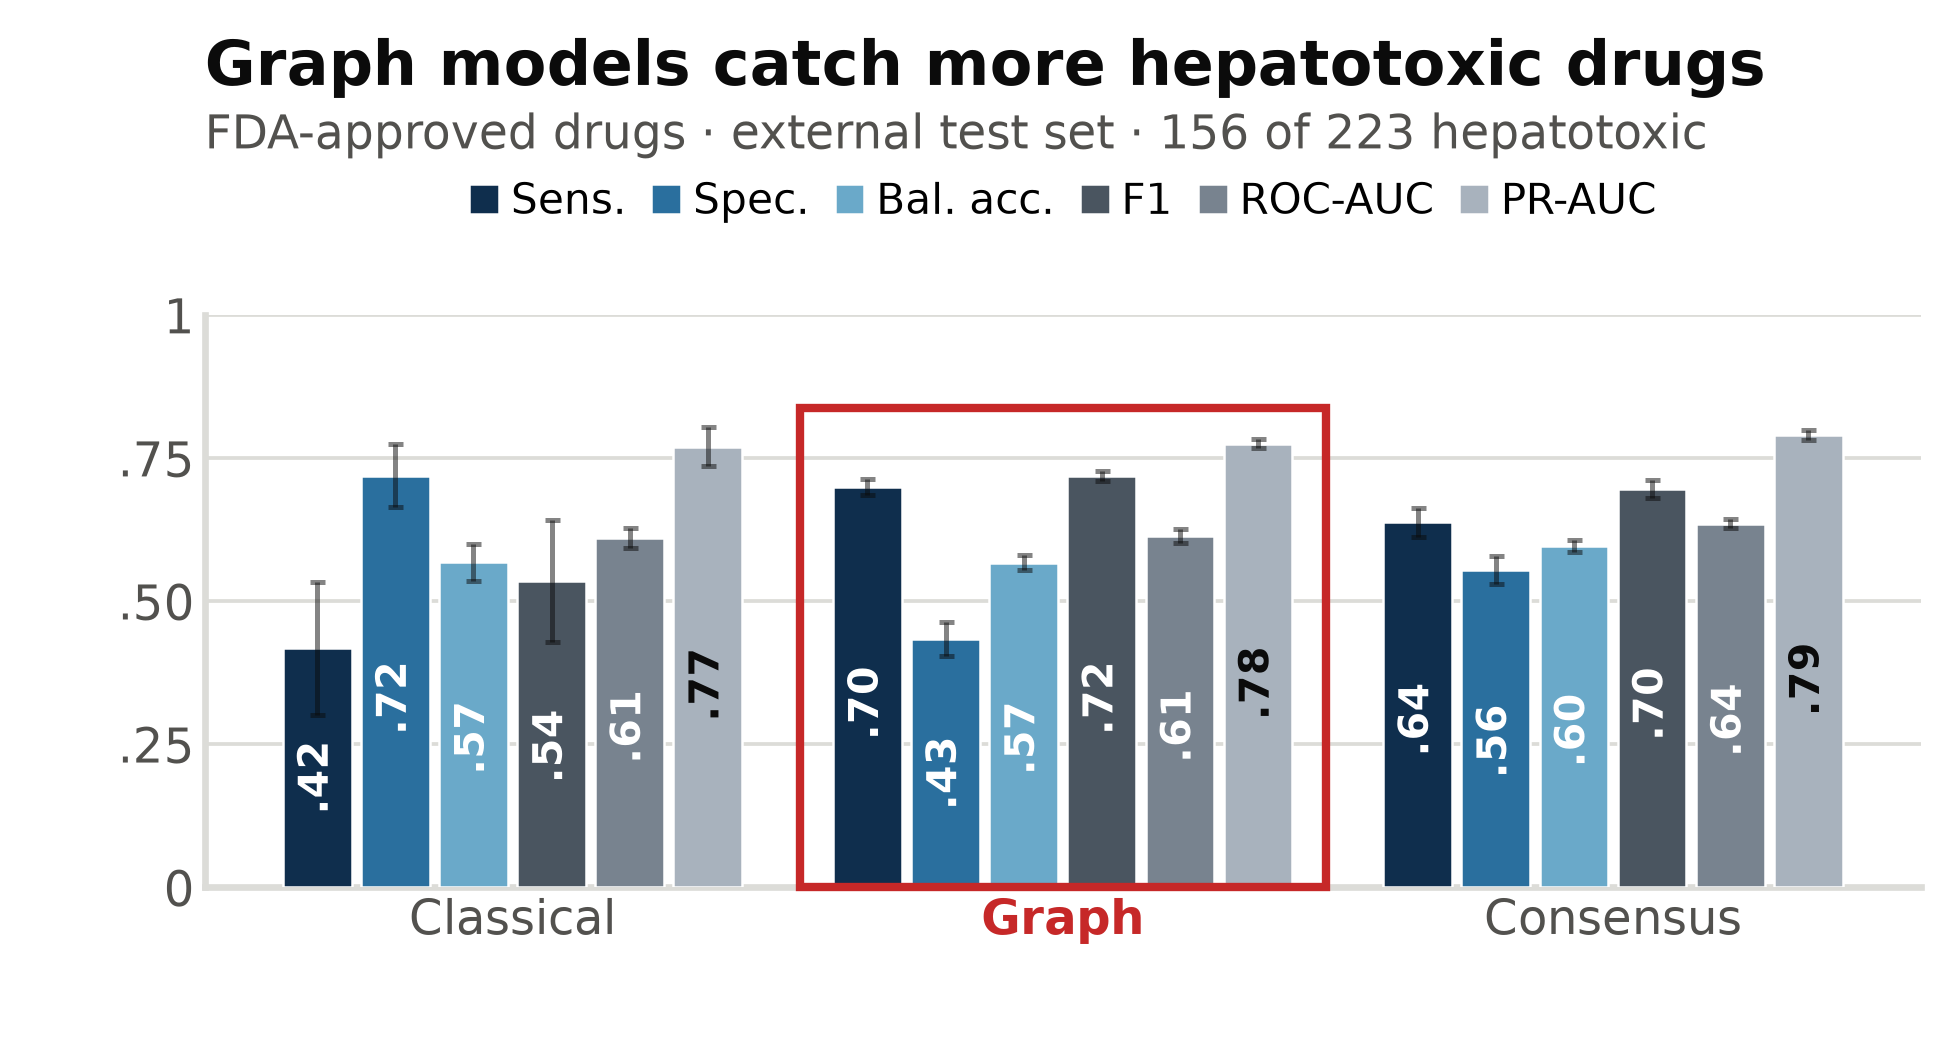
\includegraphics[width=\textwidth]{figures/dili_toc_graphic.png}
\end{figure*}

\clearpage


\begin{abstract}
Caspase-3 and -7 are key effector caspases in the apoptotic pathway, a form of programmed cell death, and their activities serve as a well-established biomarker for evaluating environmental chemical toxicity and informing chemical risk assessment. Loss of mitochondrial membrane potential is a key event in the activation of Caspase-3/7 signaling and the subsequent induction of apoptosis. Therefore, simultaneous assessment of mitochondrial membrane potential and Caspase-3/7 activity enables elucidation of the mechanisms and pathways through which apoptosis is initiated. Quantitative Structure–Activity Relationship (QSAR) modeling have been widely used for toxicity prediction. While advanced graph deep learning approaches, such as graph transformers (GTs), have shown outstanding performance in many domains, they have not been fully leveraged in QSAR modeling.
%
\end{abstract}

\section*{Keywords}

Caspase-3/7, Human hepatotoxicity, QSAR, Graph Transformers, Graph Neural Networks

% \section*{Abbreviations}

% Some journals require a list of abbreviations: these normally should be given
% immediately after the keyswords (if required).

%%%%%%%%%%%%%%%%%%%%%%%%%%%%%%%%%%%%%%%%%%%%%%%%%%%%%%%%%%%%%%%%%%%%%
%% Start the main part of the manuscript here.
%%%%%%%%%%%%%%%%%%%%%%%%%%%%%%%%%%%%%%%%%%%%%%%%%%%%%%%%%%%%%%%%%%%%%
% ============================================================
\section{Introduction}
% ============================================================

% Apoptosis is a type of programmed cell death that is crucial for maintaining homeostasis and eliminating abnormal cells. Caspase-3/7, as the core effector protease in the execution phase of apoptosis, is a key biomarker and the final common pathway for cells to irreversibly enter apoptosis. When cells are subjected to internal or external stress (such as mitochondrial dysfunction), upstream signaling pathways converge and activate Caspase-3/7, which then cleaves various cytoskeletal proteins and DNA repair enzymes, leading to characteristic morphological and biochemical changes in the cell. Environmental compounds or drugs can exert toxic effects on organisms by interfering with normal physiological processes and inducing excessive apoptosis. In evaluating such toxic effects, measuring Caspase-3/7 activity has been considered a key indicator for identifying whether a compound induces apoptotic cytotoxicity.

% Mitochondrial membrane potential (MMP) is a critical indicator for maintaining cellular energy homeostasis and survival, and its collapse is an early hallmark event in the intrinsic pathway of apoptosis. When drugs or environmental compounds induce mitochondrial damage, the decrease in membrane potential leads to the opening of mitochondrial permeability transition pores, releasing pro-apoptotic factors such as cytochrome c, which in turn activates the caspase cascade. Caspase-3/7, as downstream effectors of this pathway, are activated, marking the irreversible stage of apoptosis. Therefore, \emph{simultaneously} monitoring mitochondrial membrane potential and Caspase-3/7 activity can comprehensively capture the entire process from the initiation of mitochondrial damage to the execution of apoptosis, providing a mechanistically clear series of biomarkers for evaluating compound-induced apoptotic toxicity.

Apoptosis is a form of programmed cell death mediated by Caspase-3/7 that is crucial for maintaining internal homeostasis \cite{bursch2008cell}. As the central enzymes of the apoptotic execution phase, Caspase-3/7 constitute the common pathway through which cells irreversibly commit to apoptosis. Environmental compounds can induce excessive apoptosis by activating Caspase-3/7; therefore, monitoring their activity serves as a key indicator for assessing the apoptotic toxicity of such compounds. The collapse of mitochondrial membrane potential is an early event in intrinsic apoptosis that triggers the Caspase cascade \cite{gogvadze2006mitochondrial}. The \emph{simultaneous} monitoring of membrane potential and Caspase-3/7 activity enables the systematic capture of the entire process from mitochondrial damage to the execution of apoptosis, thereby providing mechanistically defined biomarkers for evaluating the apoptotic toxicity of compounds.

Rapid and accurate assessment of the potential toxicity of environmental chemicals and drugs remains a major challenge facing the field. Computational predictive models can serve as a powerful complement to traditional experimental methods, aiding in the prioritization and strategic direction of toxicity testing. Consequently, such models hold the promise of not only shortening testing cycles and reducing costs but also minimizing or even eliminating reliance on animal experimentation. 
Quantitative high-throughput screening (qHTS) generates full concentration--response curves for each compound, reducing false positives and false negatives relative to single-dose assays~\cite{inglese2006}. Xia~\textit{et al.}~\cite{xia2008} profiled 1,408 compounds for cytotoxicity across 13 human and rodent cell lines, showing that no single cell line can serve as a universal surrogate for organ toxicity. The Toxicology in the 21st Century (Tox21) programme subsequently scaled these assays to 10K compounds using an automated robotic platform~\cite{atteneramos2013}. The Tox21 data, publicly available in PubChem BioAssay~\cite{wang2014pubchem}, has greatly enabled the development of computational modeling for predicting \emph{in vivo} toxicity to replace costly and time-consuming animal testing.


Quantitative Structure–Activity Relationship (QSAR) modeling has been a cornerstone of computational toxicology since Hansch and Fujita~\cite{hansch1964}. QSAR models have been widely used for toxicity prediction~\cite{Tropsha2010}. Models trained on the full Tox21 10K profiles demonstrated that a combination of structural and activity data results in better models than using structure or activity data alone~\cite{Huang2016}. Deep learning algorithms have been shown to outperform classic random forest and support vector machine in Tox21 assays~\cite{Mayr2016}. For example, Kim \emph{et al.}~\cite{kim2015mechanism} studied hepatotoxicity and developed a QSAR model based on the antioxidant response element beta lactamase reporter gene assay from the Tox21. However, studies specifically targeting \emph{Caspase-3/7 activation}, a key indicator of apoptosis, remain relatively scarce.

To date, only one such report has been published, conducted by Huang~\textit{et al.}~\cite{Huang2009}, who analyzed Caspase-3/7 activation and cell viability data in Tox21 and proposed a fragment-based weighted feature significance (WFS) QSAR model. This model achieved performance comparable to Naive Bayesian models and superior to SVM, while offering improved interpretability through feature-level analysis \cite{Huang2009}. The WFS model proposed in this study constructs a simple yet highly interpretable framework for toxicity prediction by statistically quantifying the enrichment of "toxic structural features" within active compounds. Unlike methods relying on overall molecular similarity, this approach is grounded in fragment-level structural information, thereby enabling the effective prediction of toxicity for structurally diverse compounds. However, the model still presents key limitations. Its training dataset integrates high-throughput screening results derived from 13 distinct cell lines, defining "pan-cytotoxicity" through averaging or aggregation without explicitly distinguishing the biological differences among these various cell types during the modeling process. This approach implicitly assumes that the toxic effects of a compound exhibit uniformity across different cell types. However, different cells demonstrate significant variations in metabolic capacity, receptor expression (particularly upstream signaling receptors associated with Caspase-3/7 activation), and signaling pathways. Consequently, the same compound may induce distinct or even opposing toxic responses in different cellular contexts, including differential effects on cell viability and Caspase-3/7 activation.

% To a certain extent, it addresses the limitations of traditional QSAR models regarding generalization capability and mechanistic interpretability; consequently, it can be regarded as a crucial bridge connecting QSAR with mechanistic toxicology. 


Furthermore, the quality of QSAR models depends on the machine learning approach, the molecular descriptors used for the toxicity endpoint, and the quality of the training data~\cite{Huang2009}. Prior work using Tox21 qHTS data has demonstrated that models combining chemical fingerprints with bioactivity data achieve higher predictive accuracy than structure-only models, particularly for endpoints with clear mechanistic interpretations~\cite{Huang2016,Mayr2016}. However, classical fingerprint-based approaches encode molecular topology as fixed-length binary vectors and may lose structural information. {\bf Graph-based approaches} encode compounds directly as molecular graphs with atoms as nodes and bonds as edges, allowing structure-activity relationships to be learned from molecular topology without the information loss inherent in binary fingerprints~\cite{Gilmer2017}.
Classical QSAR fingerprints encode molecules as fixed-length binary vectors, discarding bond connectivity~\cite{rogers2010extended}. \emph{Graph neural networks (GNNs)} encode each compound as a molecular graph, learning representations through iterative message passing~\cite{Gilmer2017}. Multiple GNN architectures--GCN, GAT, GIN, and GraphSAGE--have been proposed with different aggregation strategies. 

The attention-based transformer architecture has demonstrated outstanding predictive performance across multiple domains \cite{vaswani2017attention}, such as topping the leaderboard in the molecular property prediction \cite{masters2022gps++}. As a key technique for the emerging large language models (LLMs), it has been fundamental for the powerful prediction capability of LLMs. Inspired by the success of transformers in natural language processing, graph transformer research applies transformers in graph data through tokenization and structural and positional encoding techniques. \emph{Graph transformers (GTs)} aggregate information from all nodes in a given graph, thus not suffering local structural bias in GNNs \cite{muller2023attending}. However, {\bf graph transformers (GTs) have not been fully leveraged in QSAR modeling on in vitro assay modeling and in vivo human hepatoxocity. To the best of our knowledge, there is no prior QSAR study on a comprehensive evaluation of fingerprint-based and graph-based approaches (GNNs and GTs) for Caspase and mitochondrial toxicity prediction}.

Moreover, applicability domain analysis has established best practices for QSAR model development~\cite{Tropsha2010}. The applicability domain defines the chemical space in which model predictions are considered reliable; compounds outside this region should be treated with caution~\cite{Zhu2016}. 


In this study, we propose a graph-based QSAR modeling pipeline that encompasses assay data preprocessing, feature representations (fingerprints and molecular graphs), and benchmarking machine learning (ML) models, including classic ML models, GNNs, advanced graph transformers, and their consensus ensembles.
The developed pipeline enabled a comprehensive study on the performance of various machine learning models as QSAR models, including three classical ML classifiers, four GNNs, two GTs, and four consensus models. Based on \emph{in vitro} Caspase and mitochondrial assays in PubChem, we applied the pipeline to predict Caspase-3/7 activation and mitochondrial membrane potential disruption. Experimental evaluations under repeated cross-validation show that no single architecture family is consistently superior across endpoints; instead, a consensus model combining classical, GNN and graph-transformer predictions gives the best or near-best performance on all three \emph{in vitro} endpoints. Since these QSAR models for predicting toxicity on \emph{in vitro} assays usually do not generalize well to \emph{in vivo} human hepatotoxicity \cite{Zhu2016}, we also conducted graph-based QSAR modeling for FDA-approved Drug-Induced Liver Injury (DILI) dataset \cite{seal2024improved}. Here, the full consensus model achieved an ROC-AUC of 0.643 and an F1 score of 0.731, exceeding the previous best model (ROC-AUC 0.63, F1 0.65) despite using only molecular graph structure, without the additional physicochemical and pharmacokinetic descriptors that model incorporated.

Moreover, the interplay between mitochondrial dysfunction and Caspase-3/7 activation remains unexplored, representing a critical gap in linking early mechanistic events to downstream toxicological outcomes.
Next, we performed a cross-assay mechanistic analysis to characterize the relationship between mitochondrial perturbation, Caspase-3/7 activation, and cell viability, providing insight into the apoptotic mechanisms induced by tested compounds. We conducted a comprehensive comparison between MMP disruption pathway and Caspase-3/7 activation to identify chemical substructures that are presented in compounds with dual activations. For example, phenolic compounds bearing a  para-hydroxyphenyl motif, as well as members of the lipophilic chain family with long alkyl chains can trigger the collapse of MMP, leading to the activation of Caspases-3 and -7. To understand the impacts of different cellular contexts on toxic responses for the same compound, we identified \emph{cell-line-specific} chemical substructures that exclusively activate Caspase-3/7 in a specific cell line but not in all other cell lines. Human embryonic kidney (HEK293) was the only cell line with a distinct structural motif: 1,1-dichloroethane and chlorobenzene. Human neuroblastoma (SK-N-SH) is uniquely impacted by an epoxide fragment and rat hepatoma (H-4-II-E) is uniquely impacted by a tetramethylcyclohexene motif and an acetaldehyde fragment. We also offered fine-grained insights into the interplay with MMP disruption and cell viability, particularly compounds with different activation outcomes in MMP and cell viability assays.







% \paragraph{Cross-Assay Mechanistic Analysis}

% Mitochondrial membrane potential disruption is an upstream event in the
% intrinsic apoptotic pathway, preceding downstream Caspase-3/7
% activation~\cite{Green1998,Elmore2007}. The Tox21 programme paired
% these endpoints specifically to enable pathway-level
% interpretation~\cite{Tice2013}. Huang~\textit{et al.}~\cite{Huang2009}
% showed that caspase activation does not universally co-occur with
% viability loss across cell lines. A systematic cross-assay integration
% spanning 14 cell lines, two species, and three mechanistic readouts has
% not previously been reported.

% ============================================================
\section{Methodology}
% ============================================================

\textbf{Figure \ref{fig:architecture}} shows an overview of our proposed QSAR modeling pipeline which we use for predicting Caspase-3/7 activation,  mitochondrial membrane
potential, and FDA DILI gold standard, and we explain the details in this section.

\begin{figure*}[t]
    \centering
    \includegraphics[width=0.8\textwidth]{figures/flowchart_arch_imp_updated.png}
    \caption{Overview of the QSAR modeling pipeline integrating data preprocessing, feature representations, and machine learning models from classic machine learning and graph-based approaches.}
    \label{fig:architecture}
\end{figure*}


\subsection{Databases: Sources and Preprocessing}

PubChem is a database of chemical molecules and their activities against biological assays, managed by the US National Institutes of Health. We downloaded from PubChem nine assays from the Tox21 database and thirteen assays from the National Center for Advancing Translational Sciences (NCATS), all in the CSV format. \textbf{Table~\ref{tab:celllines}} summarizes brief introductions on the different assays, their PubChem AID, and total number of compounds.

\begin{table}[t!]
\centering
\footnotesize
\caption{Summary of all twenty-two qHTS assays used in this study.
MMP = mitochondrial membrane potential; Viab.\ = cell-viability
counter screen.}
\label{tab:celllines}
\begin{tabular}{llrr}
\hline
\rule{0pt}{2.2ex}\textbf{Cell Line} & \textbf{Description} &
\textbf{Total} & \textbf{AID} \\
\hline
\multicolumn{4}{l}{\textit{NCATS Caspase-3/7 Assays}} \\
\hline
\rule{0pt}{2.2ex}HepG2                 & Human liver carcinoma         & 1{,}408 & 654 \\ \hline
Jurkat                & Human T-cell leukaemia        & 1{,}408 & 655 \\ \hline
HUV-EC-C              & Human vascular endothelial    & 1{,}408 & 656 \\ \hline
SH-SY5Y               & Human neuroblastoma           & 1{,}408 & 657 \\ \hline
BJ                    & Normal human fibroblast       & 1{,}408 & 658 \\ \hline
MRC-5                 & Normal human lung fibroblast  & 1{,}408 & 659 \\ \hline
Mesangial             & Mouse glomerular mesangial    & 1{,}408 & 660 \\ \hline
SK-N-SH               & Human neuroblastoma           & 1{,}408 & 661 \\ \hline
H-4-II-E              & Rat hepatoma                  & 1{,}408 & 663 \\ \hline
HEK293                & Human embryonic kidney        & 1{,}407 & 664 \\ \hline
N2a                   & Mouse neuroblastoma           & 1{,}408 & 665 \\ \hline
NIH 3T3               & Mouse embryonic fibroblast    & 1{,}408 & 666 \\ \hline
Renal Proximal Tubule & Human renal epithelial        & 1{,}408 & 667 \\[2pt]
\hline
\multicolumn{4}{l}{\textit{Tox21 Caspase-3/7 Assays}} \\
\hline
% \rule{0pt}{2.2ex}HepG2  & Human liver carcinoma                        & 9{,}667 & 1346978 \\ \hline
HepG2  & Human liver carcinoma (summary assay)        & 9{,}670 & 1347034 \\ \hline
HepG2  & Human liver carcinoma (Viab.)                 & 9{,}667 & 1346981 \\ \hline
% CHO-K1 & Chinese hamster ovary                         & 9{,}667 & 1346980 \\ \hline
CHO-K1 & Chinese hamster ovary (summary assay)         & 9{,}670 & 1347037 \\ \hline
CHO-K1 & Chinese hamster ovary (Viab.)                 & 9{,}667 & 1346979 \\[2pt]
\hline
\multicolumn{4}{l}{\textit{Tox21 MMP Assays}} \\
\hline
% \rule{0pt}{2.2ex}HepG2 & Human liver carcinoma (MMP)                & 10{,}486 & 720635 \\ \hline
HepG2 & Human liver carcinoma (MMP Viab.)           & 10{,}486 & 720634 \\ \hline
HepG2 & Human liver carcinoma (MMP summary assay)  & 10{,}337 & 720637 \\
\hline
\end{tabular}
\end{table}

From Tox21, we use the qHTS summary assay for Caspase-3/7 induction by small molecules in HepG2 cells (AID~1347034), in which replicate measurements have already been consolidated by PubChem, and the cell-viability counter screen (AID~1346981). HepG2 is a human hepatocellular carcinoma cell line widely used to model hepatotoxicity. AID~1347034 is the dataset used for all HepG2 caspase-3/7 predictive modelling in this study.


We also use a qHTS sumamry assay for Caspase-3/7 induction in CHO-K1 cells
(AID~1347037) and its cell-viability counter screen (AID~1346979).
CHO-K1 is a subclone of the parental Chinese hamster ovary (CHO) cell
line derived from the ovary of an adult female Chinese hamster; it is
widely employed in toxicology research as a \emph{non-human} mammalian
reference cell line, providing a complementary species perspective to
the human HepG2 data~\cite{ATCC_CHOK1}. AID~1347037 is the dataset used for all CHO-K1 caspase-3/7 predictive modelling in this study.

In addition, we adopt thirteen NCATS assays measure Caspase-3/7 cellular toxicity across thirteen distinct cell lines, spanning a broad range of tissue types and organisms. Combining with Tox21 assays, fourteen cell types are considered in this study. Table~\ref{tab:celllines} provides a short summary and detailed descriptions on diverse cell lines are referred to Supplementary S1.

We use the PubChem qHTS summary assay for small molecule disruptors of the MMP in HepG2 cells (AID~720637). In addition to the mitochondrial potential assay, these cells were also used to test the cytotoxicity by determining the cell viability in the culture based on the quantification of ATP present (a crucial molecule for various cellular processes). The cytotoxicity (AID~720634) was measured in the same assay well of the MMP assay, and the activity calls of the summary assay already take this viability counter-screen into account, so that compounds registering as MMP-active only as a consequence of general cytotoxicity are not labelled active. AID~720637 is the dataset used for all MMP predictive modelling in this study.

\paragraph{Activity Score and Outcome}

Each assay file includes a continuous activity score derived from the concentration-response curve fitting. When dose-response data are available, the \texttt{Fit\_LogAC50} value is used to quantify potency: it represents the logarithm (base 10) of the half-maximal activity concentration (AC50) in molar units, estimated by fitting a four-parameter Hill equation to the observed response curve. This value is then used to calculate a relative activity score by mapping the \texttt{Fit\_LogAC50} onto a scaled score range defined for each curve class, such that more potent compounds (lower AC50 values) receive higher scores. The resulting scores are normalised to the range of 0 to 100.

Activity classification follows PubChem conventions based on the
computed activity score. Compounds with a score of 0 are classified as \textit{inactive}; those with scores between 40 and 100 are classified as \textit{active}; and those with scores between 1 and 39 are classified as \textit{inconclusive}. The inconclusive category captures compounds with intermediate concentration-response behaviour that cannot be reliably assigned to either outcome.

\paragraph{Data Cleaning}

Before analysis, metadata rows were removed from each downloaded assay file. Duplicate records were then resolved by grouping all records for each assay by compound ID (\texttt{PubChem\_CID}): for a compound tested more than once, its activity score is averaged across all of its records, and its outcome (Active, Inactive or Inconclusive) is set from that averaged score. This avoids favouring the single highest-activity reading among a compound's repeats, which would systematically overstate compound activity, and keeping only one record for each compound also facilitates AI model training with a unique outcome.

\textbf{Table~\ref{tab:dedup_example}} illustrates the procedure with two representative cases from the MMP summary assay (AID~720637) raw data. In Case~1, the compound with \texttt{CID 439501} appears three times, all with the Active outcome but different scores; averaging the three scores (69, 74, 79) gives a final score of 74.0, keeping the Active call. In Case~2, the compound with \texttt{CID 727} appears eight times across three different outcomes (Inactive, Active, Inconclusive) with scores from 0 to 41; averaging all eight scores gives a final score of 16.4, which falls in the Inconclusive range, whereas the previous highest-score procedure would have called this compound Active (its single highest reading was 41). Note that the same cleaning procedure was applied to all Tox21 and NCATS assay files.

\begin{table}[t]
\centering
\small
\caption{Deduplication examples under the current score-averaging procedure. The final row of each case (shaded) is the single record kept after averaging.}
\label{tab:dedup_example}
\begin{tabular}{llc}
\toprule
\textbf{PubChem CID} & \textbf{Outcome} & \textbf{Score} \\
\midrule
\multicolumn{3}{l}{\textit{Case 1 --- Same outcome, different scores}} \\
\midrule
1215403 & Active & 69 \\
1215403 & Active & 74 \\
1215403 & Active & 79 \\
\rowcolor{yellow!15}
1215403 & Active & 74.0 \\
\midrule
\multicolumn{3}{l}{\textit{Case 2 --- Multiple outcomes for the same compound}} \\
\midrule
9290403 & Inactive & 0 \\
9290403 & Active & 41 \\
9290403 & Inconclusive & 25 \\
9290403 & Inconclusive & 5 \\
9290403 & Inactive & 0 \\
9290403 & Inconclusive & 30 \\
9290403 & Inconclusive & 5 \\
9290403 & Inconclusive & 25 \\
\rowcolor{yellow!15}
9290403 & Inconclusive & 16.4 \\
\bottomrule
\end{tabular}
\end{table}

\paragraph{Data Integration}

When multiple assays from different
sources profiled the same cell line, these assay files were merged. For example, the two
Caspase-3/7 induction datasets in HepG2 cells, one from Tox21
(AID~1347034 and another from NCATS (AID~654), were combined into a
single dataset, after which the same deduplication strategy described
above was applied. This procedure yielded our final assays for Caspase-3/7, MMP, and cell viability covering 14 distinct cell lines, as shown in \textbf{Table~\ref{tab:assay_summary}}.

As shown in Table~\ref{tab:assay_summary}, Caspase-3/7 activation rates varied substantially across multiple cell lines, ranging from 0.38\% in HUV-EC-C to 3.6\% in Jurkat cells among the 1,333-compound panels. In the combined HepG2 caspase screen (7,716 compounds), the activation rate was 3.65\% using the summary-assay version AID~1347034; in the CHO-K1 caspase screen (7,671 compounds), it was 2.23\% using the summary-assay version AID~1347037. Mitochondrial and cell viability assays exhibited significantly higher activation rates: the PubChem MMP summary assay (AID~720637) recorded 10.58\% active and 26.7\% inconclusive, removing compounds that are likely active only because of a cytotoxicity artifact rather than true MMP disruption.

\begin{table*}[t]
\centering
\small
\caption{Summary of the used qHTS assays: active, inactive, and
inconclusive compound counts with activation rates.}
\label{tab:assay_summary}
\begin{tabular}{lcrrrrr}
\hline
\textbf{Cell Line} & \textbf{Assay Type} &
\textbf{Active} & \textbf{Inactive} & \textbf{Inconclusive} &
\textbf{Total} & \textbf{Rate (\%)} \\
\hline
\multicolumn{7}{l}{\textit{Caspase-3/7 Activation Assays}} \\
\hline
HepG2                 & Caspase (654, NCATS)           &   15  & 1{,}296 &   22  & 1{,}333 &  1.13 \\
HepG2                 & Caspase (1347034, summary)     &  303  & 6{,}968 &  400  & 7{,}671 &  3.95 \\
% HepG2                 & Caspase (654+1347034, merged) &  282  & 7{,}003 &  431  & 7{,}716 &  3.65 \\
CHO-K1                & Caspase (1347037, summary)     &  171  & 7{,}325 &  175  & 7{,}671 &  2.23 \\
Jurkat                & Caspase   &   48  & 1{,}203 &   82  & 1{,}333 &  3.60 \\
HUV-EC-C              & Caspase   &    5  & 1{,}313 &   15  & 1{,}333 &  0.38 \\
SH-SY5Y               & Caspase   &   10  & 1{,}286 &   37  & 1{,}333 &  0.75 \\
BJ                    & Caspase   &    6  & 1{,}301 &   26  & 1{,}333 &  0.45 \\
MRC-5                 & Caspase   &    8  & 1{,}303 &   23  & 1{,}334 &  0.60 \\
Mesangial             & Caspase   &    8  & 1{,}299 &   27  & 1{,}334 &  0.60 \\
SK-N-SH               & Caspase   &   19  & 1{,}278 &   37  & 1{,}334 &  1.42 \\
H-4-II-E              & Caspase   &   19  & 1{,}268 &   46  & 1{,}333 &  1.43 \\
HEK293                & Caspase   &   17  & 1{,}274 &   42  & 1{,}333 &  1.28 \\
N2a                   & Caspase   &    7  & 1{,}304 &   22  & 1{,}333 &  0.53 \\
NIH 3T3               & Caspase   &   12  & 1{,}271 &   50  & 1{,}333 &  0.90 \\
Renal Proximal Tubule & Caspase   &    8  & 1{,}301 &   24  & 1{,}333 &  0.60 \\
\hline
\multicolumn{7}{l}{\textit{MMP and Cell Viability Assays}} \\
\hline
% HepG2  & MMP (720635)                & 1{,}412 & 3{,}213 & 3{,}474 & 8{,}099 & 17.43 \\
HepG2  & Cell Viability (MMP)        &   321   & 7{,}135 &   643   & 8{,}099 &  3.96 \\
HepG2  & MMP summary assay (720637) &   857   & 5{,}080 & 2{,}162 & 8{,}099 & 10.58 \\
CHO-K1 & Cell Viability             & 1{,}155 & 5{,}457 & 1{,}059 & 7{,}671 & 15.06 \\
HepG2  & Cell Viability             &   593   & 6{,}169 &   909   & 7{,}671 &  7.73 \\
\hline
\end{tabular}
\end{table*}

% ============================================================
\subsection{Feature Representations and Machine Learning Models}
% ============================================================

To illustrate the QSAR modeling pipeline, we chose two Caspase-3/7 datasets, HepG2 Caspase-3/7 activation and CHO-K1 Caspase-3/7 activation, to enable a cross-species comparison of Caspase-3/7 induction mechanisms between human hepatic and non-human ovarian cell lines. We also included the MMP dataset to confirm the feasibility of simultaneous monitoring of Caspase-3/7 activation and MMP disruption for novel compounds.

For each dataset, SMILES strings were parsed and converted to canonical form using RDKit (version 2025.09.2)~\cite{landrum2006rdkit}; entries that could not be parsed were discarded. Compounds labelled as inconclusive (activity scores 1--39) were excluded during model training. After the processing, the HepG2 Caspase-3/7 dataset retained 7,285 compounds with 282 active (3.9\%) and 7,003 inactive (96.1\%) compounds, indicating a severe imbalance of 24.8:1. The CHO-K1 Caspase-3/7 dataset retained 7,496 compounds with 171 active (2.3\%) and 7,325 inactive (97.7\%) compounds, reflecting a more severe imbalance of 42.8:1. The mitochondrial toxicity dataset retained 5,937 compounds with 857 active (14.4\%) and 5,080 inactive (85.6\%) compounds.

\paragraph{Molecular Feature Representation}

We apply a two-track feature engineering strategy to construct both feature representations, molecular fingerprints and molecular graphs, for classical machine learning and graph-based deep learning approaches.

{\noindent \em Morgan Fingerprints (ECFP4).}
Extended-connectivity fingerprints with radius 2 and 2,048 bits (ECFP4)~\cite{rogers2010extended} were generated for each compound using RDKit (version 2025.09.2). These circular fingerprints encode the local atomic environment up to two bond distances from each atom and serve as widely used molecular descriptors in QSAR modeling.

{\noindent \em Molecular Graph Representation.}
For the graph-based learning track, each compound was encoded as a directed molecular graph with atoms as nodes and bonds as edges; all bonds were represented bidirectionally to enable symmetric message passing. Each atom node was described by a 27-dimensional feature vector encoding atom types (C, N, O, S, F, P, Cl, Br, I, or other; one-hot encoding), degree (0--5; one-hot encoding), formal charge, hybridisation state (sp, sp$^2$, sp$^3$, or other; one-hot encoding), aromaticity, ring membership, total hydrogen count, and scaled atomic mass. Each bond edge was described by a 6-dimensional feature vector encoding bond type (one-hot encoding), conjugation status, and ring membership.

\paragraph{Data Partitioning}

Each dataset was evaluated under three partitioning schemes.

\emph{Repeated random split.} Each dataset was split using two sequential
stratified splits: 10\% was held out as the test set, and the remaining 90\%
was split into 80\% train and 10\% validation. This was repeated five times,
each with a separate random seed, giving the random split the same kind of
spread of results already reported for the 10-fold and scaffold-split
schemes below.

\emph{10-fold cross-validation.} Each dataset was divided into ten stratified
folds. This was repeated ten times: in each round, one fold served as the
test set and a second fold as the validation set, rotating so that every
compound was used as a test compound exactly once.

\emph{Scaffold split.} Compounds were grouped by Bemis--Murcko scaffold~\cite{bemis1996properties} --- the ring systems of a molecule together with the acyclic linkers joining them, obtained by removing all terminal side chains, and computed from the molecular graph without stereochemistry --- and whole scaffold groups were assigned to training, validation or test, so no scaffold appeared in more than one set.  Bin sizes are strongly skewed: binning gave 1,932 bins for the HepG2 caspase-3/7 dataset, 1,988 for CHO-K1 and 1,686 for the MMP assay, with roughly one fifth of compounds in singleton bins. We used the bin-assignment heuristic of Yang~\textit{et al.}~\cite{yang2019analyzing}, as adopted for MV-GNN by Ma~\textit{et al.}~\cite{ma2022cross}, with 8:1:1 target proportions. Any bin larger than half the desired test-set size, that is above 5\% of the dataset, goes straight to training, which protects scaffold diversity in the held-out sets; in all three datasets exactly two bins qualify, the acyclic bin with an empty scaffold and the benzene bin, together about 45\% of each dataset. The remaining bins are shuffled with a repeat-specific seed and filled bin by bin into the test set, then the validation set, with the rest going to training. The split is not stratified, so held-out class ratios follow the bins: across the five CHO-K1 repeats the test sets held 20 to 35 actives (2.7--4.7\% against 2.3\% overall), leaving only 112 to 130 of the 171 actives for training. The procedure was repeated five times with a fresh shuffle, and reported values are means over the five repeats.

Scaffold split is a more challenging setting than random splitting, as
Yang~\textit{et al.}~\cite{yang2019analyzing} note, and it is the protocol
MV-GNN$^{\text{cross}}$~\cite{ma2020multiview,ma2022cross} is evaluated under.
Because held-out compounds carry Bemis--Murcko scaffolds absent from training,
the model must generalize across chemical series rather than interpolate
within them, and because the split is not stratified, fewer actives reach the
training set, leaving a smaller balanced training set. ROC-AUC is accordingly
lower under the scaffold split than under the repeated random split or the
10-fold cross-validation for every model on all three datasets, so all three
protocols are reported for better comparison. Validation and test sets kept
their natural class ratios under all three schemes; balancing was applied to
the training set only.

\paragraph{Class Balancing}

All three \emph{in vitro} endpoints are class-imbalanced, with
inactive-to-active ratios of 5.9:1 for the MMP summary assay (857 active,
5,080 inactive), 24.8:1 for HepG2 Caspase-3/7 (282 active, 7,003 inactive)
and 42.8:1 for CHO-K1 Caspase-3/7 (171 active, 7,325 inactive) in the
curated datasets (Supplementary Table~S1). Two balancing strategies were
evaluated on the training set: random majority-class downsampling, and
random up-sampling of the active class, in which active compounds are drawn
with replacement until they match the inactive count so that no inactive
compound is discarded. Balancing was applied to the training set only;
validation and test sets retained the natural class ratio of each dataset.
Because the training set holds 80\% of the compounds under the random split,
the counts below are drawn from 685 of the 857 MMP actives, 226 of the 282
HepG2 actives and 137 of the 171 CHO-K1 actives.

Under the 80:10:10 random split, downsampling to a 1:1 ratio gives a
training set of 1,370 compounds (685 active, 685 inactive) for the MMP
summary assay, 452 compounds (226 active, 226 inactive) for HepG2
Caspase-3/7 and 274 compounds (137 active, 137 inactive) for CHO-K1
Caspase-3/7; the split is stratified, so these counts are identical across
repeats. Up-sampling to the same 1:1 ratio instead retains every inactive
compound, giving 8,128 compounds (4,064 active, 4,064 inactive) for the MMP
summary assay, 11,202 compounds (5,601 active, 5,601 inactive) for HepG2
Caspase-3/7 and 11,718 compounds (5,859 active, 5,859 inactive) for CHO-K1
Caspase-3/7. Scaffold splits are not stratified, so the corresponding
training-set sizes vary by a few tens of compounds between repeats. A 1:5
downsampling ratio was additionally evaluated on CHO-K1 Caspase-3/7 under
the scaffold split, giving a mean of 720 training compounds (120 active, 600
inactive) across the five repeats, ranging from 672 to 780.

Both strategies were run under all three partitioning schemes for each
assay. Under 10-fold cross-validation, up-sampling gave a higher mean
ROC-AUC than 1:1 downsampling across all models on every assay, by 0.022 on
the MMP summary assay (0.887 to 0.909), 0.028 on HepG2 (0.841 to 0.869) and
0.022 on CHO-K1 (0.779 to 0.801), with correspondingly larger differences in
PR-AUC (0.617 to 0.699, 0.244 to 0.362, and 0.117 to 0.212 respectively).
Up-sampled results are therefore reported in the main text, with the 1:1
downsampled results given alongside them for every assay and partitioning
scheme in Supplementary Tables~S2--S5.


\paragraph{Uncertainty and Statistical Comparison}

For 10-fold cross-validation and the repeated scaffold split, 95\%
confidence intervals for ROC-AUC and PR-AUC were computed from the ten fold
values or five repeat values using a paired $t$-interval with the
Nadeau--Bengio correction. Comparisons between models were made with a
paired test across folds, with $p$-values corrected for multiple comparisons
using the Holm method.

\paragraph{Classical Machine Learning}

Three classical machine learning algorithms were trained and evaluated on the datasets under a grid-search hyperparameter optimisation protocol: Random Forest~\cite{breiman2001random} and Support Vector Machine (SVM) with an RBF kernel~\cite{cortes1995support} (both scikit-learn, version 1.6.1), and XGBoost~\cite{chen2016xgboost} (xgboost, version 2.1.4). All models were trained on the balanced training sets, and hyperparameters were optimised using ROC-AUC on the imbalanced validation set. Full hyperparameter configurations are provided in Supplementary S1.%\ref{apx:hyperparameter}.
We added one more method, chemical-structure-only workflow of Xu~\textit{et al.}~\cite{xu2026expanded}
couples ECFP4 fingerprints with a feature selection step and a classical
classifier, searching over four feature selection methods, five classifiers, and
four training-set resampling variants to select one configuration on validation
ROC-AUC; the configuration selected here was Random Forest feature selection
with an RBF SVM. It is replicated as an external baseline because that study
reported chemical structure alone to perform on par with chemical structure
combined with the full Tox21 assay panel for DILI prediction

\paragraph{Graph Neural Networks}

Four representative message-passing graph neural network architectures were trained and evaluated: Graph Convolutional Network (GCN)~\cite{kipf2016semi}, Graph Attention Network (GAT)~\cite{velivckovic2017graph}, Graph Isomorphism Network (GIN)~\cite{xu2018powerful}, and GraphSAGE~\cite{hamilton2017inductive}. All four architectures were implemented within a shared modular framework built on PyTorch Geometric (version 2.6.1)~\cite{fey2019fast}, using the \texttt{GCNConv}, \texttt{GATConv}, \texttt{GINConv}, and \texttt{SAGEConv} layer primitives, respectively. Input atom features were projected to a hidden dimension via a linear layer with batch normalisation and ReLU activation, followed by three to four message-passing layers, each equipped with batch normalisation, ReLU activation, dropout, and a residual skip connection. Global mean pooling produced a fixed-length graph-level embedding passed to a two-layer MLP classification head trained with binary cross-entropy loss. GAT incorporated multi-head attention with 4 or 8 heads; GIN employed a learnable parameter $\varepsilon$ and an internal two-layer MLP for neighbour aggregation. MV-GNN$^{\text{cross}}$~\cite{ma2020multiview}, termed CD-MVGNN in the published version of that work~\cite{ma2022cross}, is a multi-view message passing architecture with both atom-central encoder and bond-central encoder and uses the self-attentive aggregation to learn different weights of the atom/bond embeddings to produce the final graph embedding. It also allows information communication of the two views to improve the expressive power.

\paragraph{Graph Transformers}

Graph transformers overcome the locality bias of message-passing GNNs by incorporating global attention that allows every node to attend to every other node simultaneously, avoiding the over-smoothing and limited receptive-field problems inherent in the iterative neighbourhood aggregation~\cite{muller2023attending}. Two representative architectures were implemented: Graphormer \cite{ying2021transformers} and GraphGPS \cite{rampavsek2022recipe}. See their architectural details in Supplementary S1.%\ref{apx:gt}.

Both models share a two-layer MLP classification head (256~$\to$~128~$\to$~1) trained with class-ratio-weighted binary cross-entropy loss, the Adam optimiser, and a ReduceLROnPlateau scheduler (factor~$=0.5$, patience~$=5$). Early stopping (patience~$=15$, maximum 100~epochs) and a batch size of 64 were used consistently. Full hyperparameter settings are reported in Supplementary S1.%\ref{apx:hyperparameter}.


\paragraph{Consensus Models}

A consensus ensemble strategy was implemented, which aggregates the predictions of individual models to reach a "consensus", and usually enhances accuracy by mitigating individual model errors. The full consensus prediction was calculated as the arithmetic mean of the predicted active probabilities from all nine trained models: Random Forest, SVM, XGBoost, GCN, GAT, GIN, GraphSAGE, Graphormer, and GraphGPS. Three consensus ensemble variants were evaluated: a classical consensus (RF, SVM, and XGBoost), a GNN consensus (GCN, GAT, GIN, and GraphSAGE), and a GT consensus (Graphormer and GraphGPS).

\paragraph{In vivo FDA-approved DILI Prediction}

We evaluated our graph-based pipeline on the FDA-approved Drug-Induced Liver Injury (DILI) dataset, comprising 1,111 compounds from DILIst \cite{thakkar2020drug} and DILIrank \cite{chen2016dilirank} that have been classified as inducing DILI or not and were developed from FDA-approved drug labels. Briefly, DILIrank categorizes drugs into four classes by combining FDA drug labeling information with verified causality evidence from published assessments~\cite{chen2016dilirank}: Most-DILI-concern, Less-DILI-concern, No-DILI-concern, and an Ambiguous DILI-concern category for drugs with unclear or conflicting annotations. DILIst extends this scheme by incorporating additional drugs from independent DILI annotation sources (clinical case registries, literature evidence, and the FDA Adverse Event Reporting System) where sufficient agreement with existing annotations was found, and defines a binary label by combining the Most- and Less-DILI-concern categories as DILI-positive and the No-DILI-concern category as DILI-negative, with Ambiguous-concern drugs excluded~\cite{thakkar2020drug}. As in Seal et al.~\cite{seal2024improved}, the data was partitioned into the \emph{DILI training} set of 888 compounds and the \emph{DILI held-out test} set of 223 compounds using a scaffold-based method (based on the Butina clustering of a bulk Tanimoto fingerprint matrix split with a cutoff threshold of 0.70). This ensures that the DILI test set included a wide variety of compounds that are structurally less similar to those used in training, representing a more challenging split compared to random splits yet matching practical scenarios. We performed SMILES canonicalization using RDKit (version 2025.09.2), removed those compounds that cannot be parsed, and resulted in the DILI training set of 874 compounds (with 553 hepatotoxic and 321 non-hepatotoxic compounds) and the DILI held-out test set of 222 compounds (with 155 hepatotoxic and 67 non-hepatotoxic compounds). We also incorporated the same training data from \cite{seal2024improved}, which uses different in vivo and in vitro data sources, such as liver injury end points for human, preclinical, and animal hepatotoxicity, DILI datasets compiled by various studies, and in vitro assays on mitochondrial toxicity, bile salt export pump inhibition, and the formation of reactive metabolites. This training data is called the \emph{Proxy-DILI} data: after deduplication and removing all 1,111 gold-standard compounds, there are 12,900 unique compounds (active: 4,217; inactive: 8,683). 

We trained all nine base models -- three classical classifiers (RF, SVM, XGBoost), four graph neural networks (GCN, GAT, GIN, GraphSAGE), and two graph transformers (Graphormer, GraphGPS) -- under two settings: \textit{Proxy-only} with only the \emph{Proxy-DILI} data of 12,900 compounds as the training data and \textit{Proxy+DILI} combining the Proxy-DILI and the DILI training data. Each model family was evaluated using 5-fold cross-validation with ensembling: for the graph-based models, each fold's Proxy-only model was pretrained on that fold's 12,900-compound Proxy-DILI training split, and the Proxy+DILI model was obtained by further fine-tuning on the DILI training data; for the classical models, each fold's Proxy+DILI model was independently retrained on the combined data. Evaluations on the same held-out DILI test set under the same two settings enable a fair comparison of the selected models for their predictive performance for in vivo FDA data. Consensus models (Classical, GNN, GT, and the full nine-model consensus) were also built and evaluated to confirm their advantages. 

%minus the held-out 223 (DILI$+$: 4,650; DILI$-$: 8,959) with supervised DILI labels at $\eta=10^{-3}$ for 80 epochs, followed by Stage~2 fine-tuning on the clinical split at $\eta=3\times10^{-4}$ for 60 epochs.

% Transfer-learning GNNs (TL-GIN, TL-GAT) were pretrained on $\sim$307K compounds from seven qHTS bioactivity assays (mitochondrial toxicity, HepG2 caspase cytotoxicity, BSEP inhibition, reactive metabolite formation, ARE-bla oxidative stress, thyroid receptor antagonism, and PPAR$\gamma$ activation; PubChem AID 720635, 686978, 743202, 651741, 743067, and 743140), then fine-tuned on the clinical partition at $\eta = 3\times10^{-4}$.

% Ensemble predictions were formed via consensus averaging of three subsets of base models (3-way: RF-aug + XGB-aug + TL-GIN; 4-way: additionally TL-GAT-aug; 6-way: additionally Graphormer-aug + GraphGPS-aug) and via a logistic-regression stacking meta-learner trained on 5-fold out-of-fold predictions. All metrics are reported on the fixed held-out 222 compound test set.


\paragraph{Applicability Domain}

The applicability domain (\emph{AD}) defines the region of chemical space in
which a model's predictions can be considered reliable~\cite{Zhu2016}.
An AD was defined independently for each dataset using a 5-nearest-neighbour (5-NN) Jaccard distance criterion applied to the binary
ECFP4 training fingerprints. For each training compound $i$, the mean
5-NN Jaccard distance $\bar{d}_i$ was calculated by:
    $\bar{d}_i = \frac{1}{5}\sum_{j=1}^{5} d_{i,j}$.
The AD threshold $\theta$ was set at the mean plus 1.5 standard
deviations of the training distribution:
\begin{equation*}
    \theta = \frac{1}{N}\sum_{i=1}^{N}\bar{d}_i
           \;+\; 1.5 \times \mathrm{SD}\!\left(\{\bar{d}_i\}\right)
\end{equation*}
Test compounds with $\bar{d}_q > \theta$ were flagged as outside the
AD and their predictions treated with caution~\cite{Zhu2016}.

\paragraph{Evaluation Metrics}

All models were evaluated at two decision thresholds: a standard
threshold of 0.50 (CPT-1) and a high-confidence threshold of 0.80
(CPT-2). A comprehensive set of performance metrics was chosen and reported: \emph{Sensitivity}, \emph{Specificity}, \emph{Correct
Classification Rate (CCR $=$ (sensitivity $+$ specificity) $/ 2$)},
\emph{Receiver Operating Characteristic - Area Under Curve (ROC-AUC)}, \emph{Area Under the Precision-Recall Curve (PR-AUC)}, \emph{Matthews correlation coefficient (MCC)}, and \emph{F1-score}.
We choose the widely adopted ROC-AUC and F1-score as the primary performance measures.



% ============================================================
\section{Results and discussions}
\label{sec:results}
% ============================================================




% ============================================================
% ============================================================
\subsection{Prediction Results of QSAR Models}
% ============================================================

\subsubsection*{Mitochondrial Toxicity Dataset}

Mitochondrial membrane potential (MMP) plays a central role in maintaining
cellular energy homeostasis and survival, and its loss is an early initiating
event in the intrinsic apoptotic pathway leading to Caspase-3/7 activation.
For MMP modelling we use the PubChem MMP summary assay (AID~720637), in which
the activity calls already take the parallel cell-viability counter screen into
account, so that compounds registering as MMP-active only as a consequence of
general cytotoxicity are not labelled active. The raw MMP assay (AID~720635)
and its viability counter screen (AID~720634) are retained for the cross-assay
analysis reported later in this section, where the relationship between MMP
disruption, Caspase-3/7 activation and cell viability is examined directly.

\begin{table*}[t]
\centering
\caption{Performance on the MMP summary assay (AID 720637) under 10-fold cross-validation. In each of ten rounds, one fold was the test set, the next fold the validation set, and the remaining eight folds the training set, with actives up-sampled to a 1:1 ratio. Values are the mean of the ten test-fold scores.}

\label{tab:mmp_up_loo}
\resizebox{\textwidth}{!}{%
\begin{tabular}{llccccccc}
\toprule
\textbf{Model} & \textbf{CPT} & \textbf{Sensitivity} & \textbf{Specificity} & \textbf{CCR} & \textbf{ROC-AUC} & \textbf{PR-AUC} & \textbf{MCC} & \textbf{F1} \\
 & & (\%) & (\%) & (\%) & & & & \\
\midrule
\multicolumn{9}{l}{\textit{Classical Machine Learning}} \\
\midrule
\multirow{2}{*}{Random Forest} & 0.5 & $54.02 \pm 5.00$ & $95.75 \pm 2.85$ & $74.89 \pm 1.69$ & \multirow{2}{*}{$0.897 \pm 0.026$} & \multirow{2}{*}{$0.678 \pm 0.051$} & $0.556 \pm 0.045$ & $0.605 \pm 0.034$ \\
 & 0.8 & $19.61 \pm 7.15$ & {\boldmath$99.49 \pm 0.39$} & $59.55 \pm 3.44$ &  &  & $0.374 \pm 0.072$ & $0.314 \pm 0.099$ \\
\multirow{2}{*}{SVM} & 0.5 & $48.31 \pm 8.67$ & $97.48 \pm 0.90$ & $72.90 \pm 4.02$ & \multirow{2}{*}{$0.903 \pm 0.023$} & \multirow{2}{*}{$0.701 \pm 0.046$} & $0.559 \pm 0.055$ & $0.588 \pm 0.065$ \\
 & 0.8 & $36.18 \pm 8.46$ & $98.74 \pm 0.51$ & $67.46 \pm 4.12$ &  &  & $0.503 \pm 0.071$ & $0.499 \pm 0.088$ \\
\multirow{2}{*}{XGBoost} & 0.5 & $65.47 \pm 5.13$ & $92.60 \pm 2.12$ & $79.04 \pm 2.94$ & \multirow{2}{*}{$0.891 \pm 0.024$} & \multirow{2}{*}{$0.674 \pm 0.060$} & $0.562 \pm 0.064$ & $0.627 \pm 0.053$ \\
 & 0.8 & $43.53 \pm 5.47$ & $97.85 \pm 0.65$ & $70.69 \pm 2.78$ &  &  & $0.532 \pm 0.055$ & $0.556 \pm 0.053$ \\
\midrule
\multicolumn{9}{l}{\textit{Graph Neural Networks}} \\
\midrule
\multirow{2}{*}{GCN} & 0.5 & $81.46 \pm 4.88$ & $87.66 \pm 3.10$ & $84.56 \pm 2.28$ & \multirow{2}{*}{$0.915 \pm 0.018$} & \multirow{2}{*}{$0.691 \pm 0.072$} & $0.586 \pm 0.048$ & $0.642 \pm 0.042$ \\
 & 0.8 & $66.64 \pm 7.08$ & $95.14 \pm 1.36$ & $80.89 \pm 3.48$ &  &  & $0.631 \pm 0.057$ & $0.681 \pm 0.049$ \\
\multirow{2}{*}{GAT} & 0.5 & $80.74 \pm 3.85$ & $86.42 \pm 1.97$ & $83.58 \pm 1.84$ & \multirow{2}{*}{$0.906 \pm 0.017$} & \multirow{2}{*}{$0.681 \pm 0.077$} & $0.560 \pm 0.034$ & $0.619 \pm 0.029$ \\
 & 0.8 & $68.14 \pm 6.29$ & $93.90 \pm 1.19$ & $81.02 \pm 2.80$ &  &  & $0.610 \pm 0.036$ & $0.666 \pm 0.032$ \\
\multirow{2}{*}{GIN} & 0.5 & $77.14 \pm 4.89$ & $91.69 \pm 2.17$ & $84.41 \pm 2.40$ & \multirow{2}{*}{$0.923 \pm 0.017$} & \multirow{2}{*}{$0.728 \pm 0.058$} & $0.628 \pm 0.049$ & $0.683 \pm 0.041$ \\
 & 0.8 & $67.22 \pm 6.05$ & $95.73 \pm 1.25$ & $81.47 \pm 2.79$ &  &  & \underline{$0.651 \pm 0.042$} & \underline{$0.698 \pm 0.039$} \\
\multirow{2}{*}{SAGE} & 0.5 & $79.00 \pm 5.67$ & $89.21 \pm 2.89$ & $84.11 \pm 2.55$ & \multirow{2}{*}{$0.912 \pm 0.019$} & \multirow{2}{*}{$0.700 \pm 0.072$} & $0.595 \pm 0.048$ & $0.652 \pm 0.041$ \\
 & 0.8 & $63.12 \pm 5.80$ & $95.53 \pm 0.78$ & $79.33 \pm 2.82$ &  &  & $0.614 \pm 0.043$ & $0.665 \pm 0.039$ \\
\midrule
\multicolumn{9}{l}{\textit{Multi-View Graph Neural Network}} \\
\midrule
\multirow{2}{*}{MV-GNN-cross} & 0.5 & $78.18 \pm 8.31$ & $89.25 \pm 4.88$ & $83.71 \pm 3.35$ & \multirow{2}{*}{$0.907 \pm 0.026$} & \multirow{2}{*}{$0.697 \pm 0.062$} & $0.595 \pm 0.066$ & $0.651 \pm 0.059$ \\
 & 0.8 & $64.05 \pm 6.79$ & $95.65 \pm 1.78$ & $79.85 \pm 2.95$ &  &  & $0.627 \pm 0.047$ & $0.674 \pm 0.042$ \\
\midrule
\multicolumn{9}{l}{\textit{Graph Transformers}} \\
\midrule
\multirow{2}{*}{Graphormer} & 0.5 & $85.41 \pm 5.45$ & $74.98 \pm 7.28$ & $80.20 \pm 2.98$ & \multirow{2}{*}{$0.880 \pm 0.027$} & \multirow{2}{*}{$0.607 \pm 0.075$} & $0.455 \pm 0.059$ & $0.517 \pm 0.054$ \\
 & 0.8 & $72.23 \pm 8.73$ & $85.96 \pm 4.53$ & $79.10 \pm 3.98$ &  &  & $0.495 \pm 0.072$ & $0.568 \pm 0.060$ \\
\multirow{2}{*}{GraphGPS} & 0.5 & \underline{$86.23 \pm 4.05$} & $81.22 \pm 5.13$ & $83.73 \pm 2.41$ & \multirow{2}{*}{$0.914 \pm 0.017$} & \multirow{2}{*}{$0.707 \pm 0.043$} & $0.530 \pm 0.058$ & $0.584 \pm 0.053$ \\
 & 0.8 & $78.18 \pm 5.68$ & $88.72 \pm 4.06$ & $83.45 \pm 2.36$ &  &  & $0.584 \pm 0.056$ & $0.642 \pm 0.049$ \\
\midrule
\multicolumn{9}{l}{\textit{Consensus Ensembles}} \\
\midrule
\multirow{2}{*}{Consensus-Classical} & 0.5 & $52.98 \pm 6.21$ & $96.69 \pm 1.21$ & $74.83 \pm 2.90$ & \multirow{2}{*}{$0.903 \pm 0.024$} & \multirow{2}{*}{$0.703 \pm 0.050$} & $0.571 \pm 0.047$ & $0.613 \pm 0.045$ \\
 & 0.8 & $32.33 \pm 5.85$ & \underline{$99.17 \pm 0.28$} & $65.75 \pm 2.93$ &  &  & $0.489 \pm 0.057$ & $0.469 \pm 0.066$ \\
\multirow{2}{*}{Consensus-GNN} & 0.5 & $80.16 \pm 4.46$ & $90.79 \pm 1.57$ & {\boldmath$85.48 \pm 2.05$} & \multirow{2}{*}{\underline{$0.924 \pm 0.016$}} & \multirow{2}{*}{\underline{$0.737 \pm 0.075$}} & $0.631 \pm 0.034$ & $0.683 \pm 0.028$ \\
 & 0.8 & $63.37 \pm 5.99$ & $96.63 \pm 0.94$ & $80.00 \pm 3.00$ &  &  & $0.649 \pm 0.052$ & $0.691 \pm 0.047$ \\
\multirow{2}{*}{Consensus-GT} & 0.5 & {\boldmath$86.82 \pm 4.35$} & $81.81 \pm 5.90$ & $84.31 \pm 3.07$ & \multirow{2}{*}{$0.916 \pm 0.019$} & \multirow{2}{*}{$0.707 \pm 0.059$} & $0.543 \pm 0.070$ & $0.595 \pm 0.064$ \\
 & 0.8 & $72.22 \pm 6.51$ & $91.89 \pm 3.20$ & $82.06 \pm 2.91$ &  &  & $0.600 \pm 0.060$ & $0.658 \pm 0.050$ \\
\multirow{2}{*}{Consensus (Full)} & 0.5 & $77.60 \pm 5.07$ & $92.91 \pm 1.51$ & \underline{$85.26 \pm 2.49$} & \multirow{2}{*}{{\boldmath$0.932 \pm 0.016$}} & \multirow{2}{*}{{\boldmath$0.772 \pm 0.051$}} & {\boldmath$0.657 \pm 0.043$} & {\boldmath$0.707 \pm 0.036$} \\
 & 0.8 & $46.10 \pm 5.97$ & $98.64 \pm 0.75$ & $72.37 \pm 2.97$ &  &  & $0.586 \pm 0.054$ & $0.597 \pm 0.055$ \\
\bottomrule
\end{tabular}%
}
\end{table*}


\FloatBarrier

\begin{figure*}[t]
    \centering
    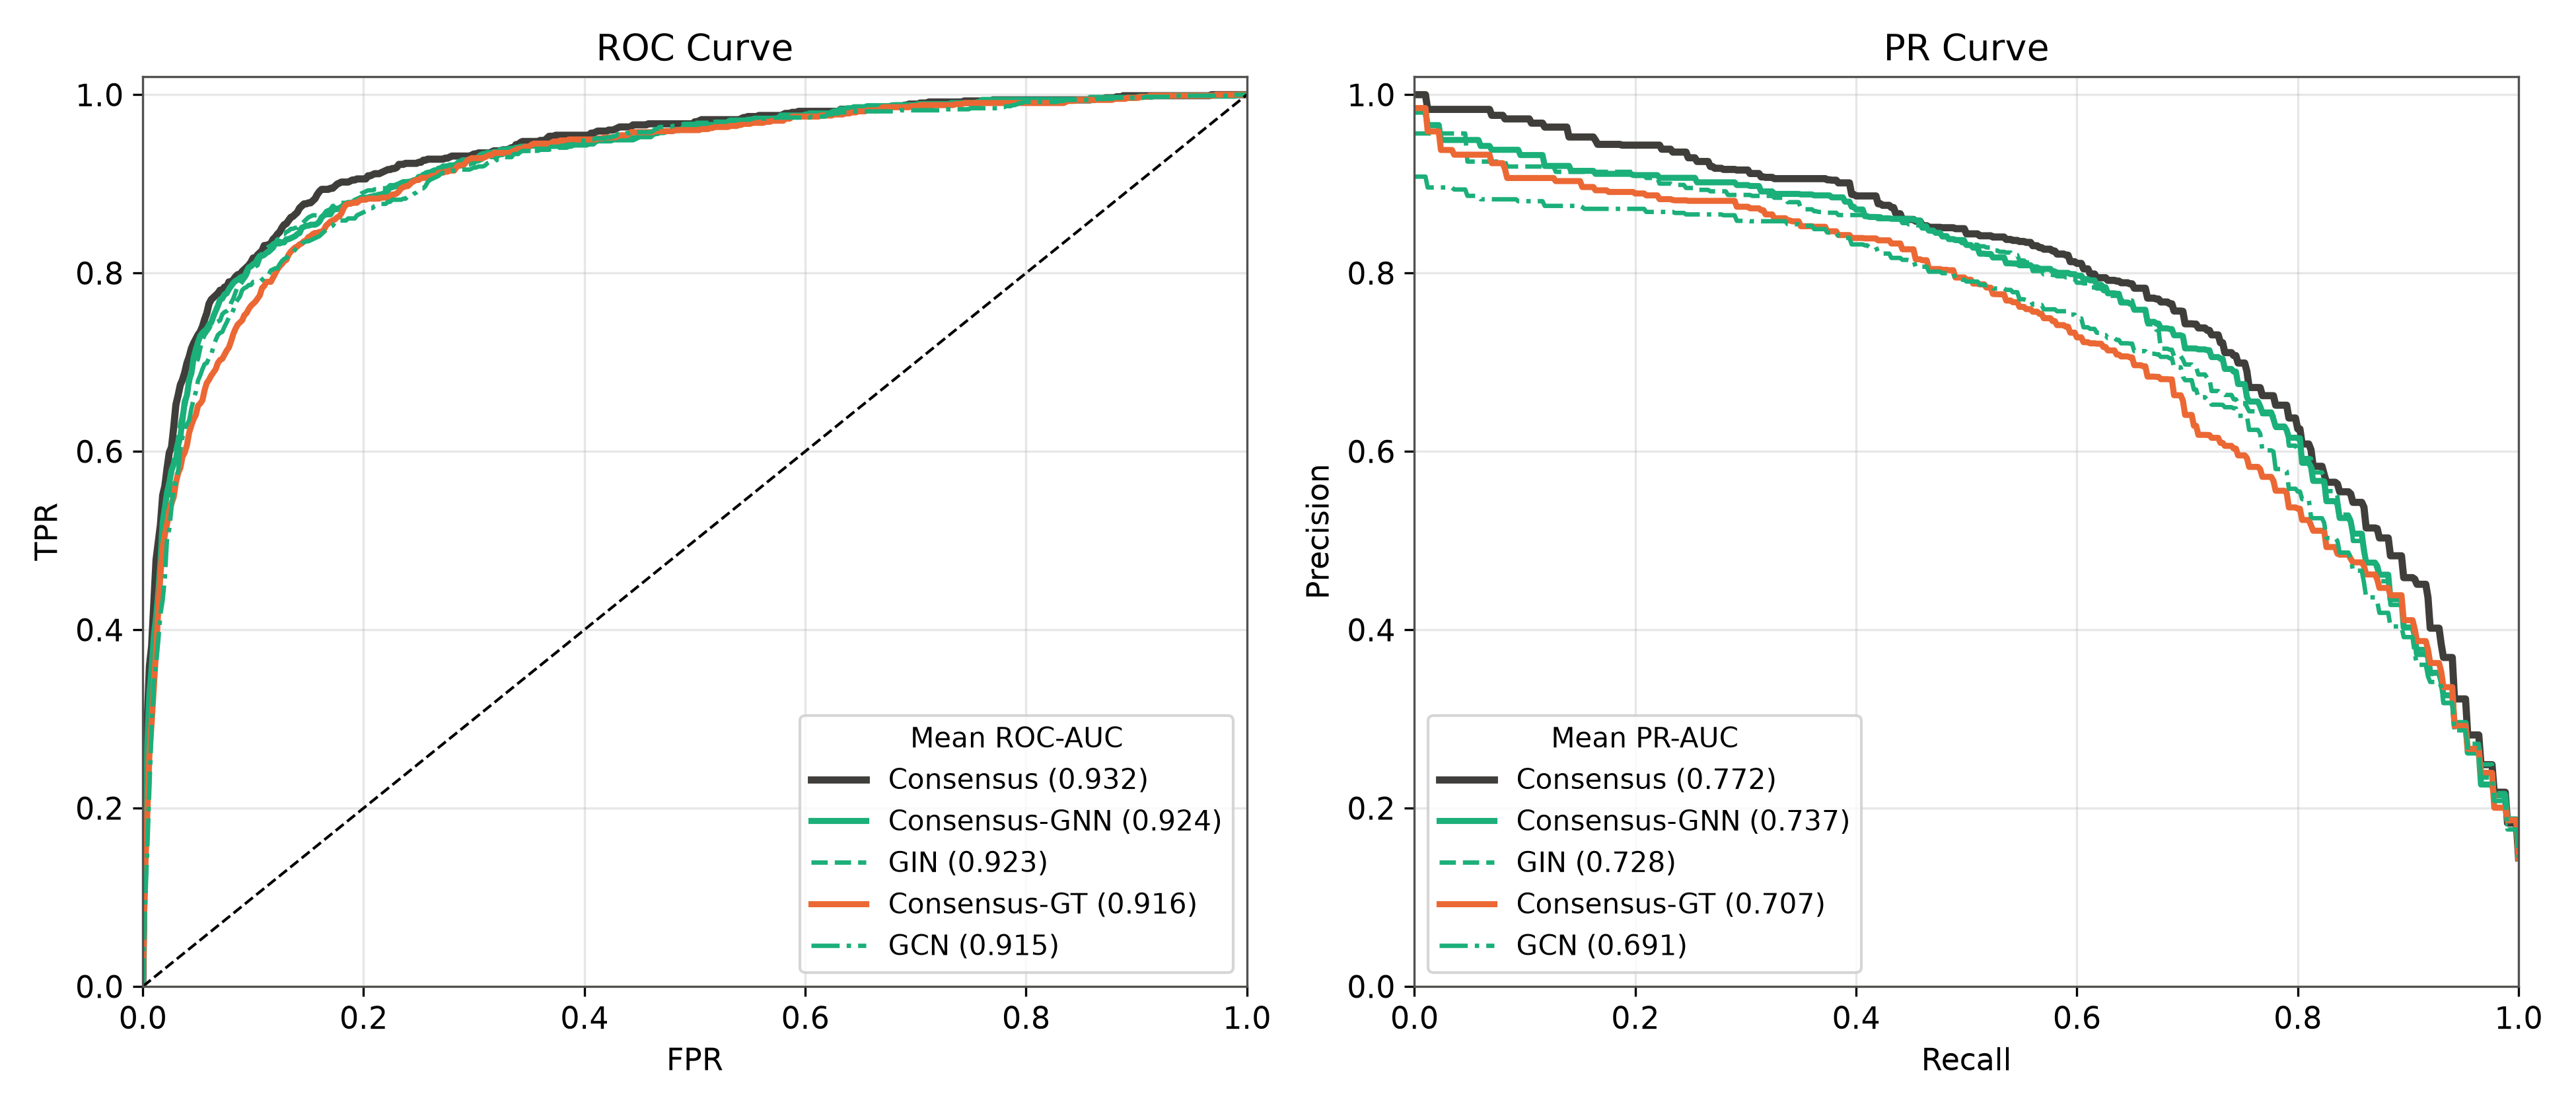
\includegraphics[width=\linewidth]{figures/mmp_cv_upsampling_roc_pr.png}
    \caption{(A) ROC Curve and (B) PR Curve for top 5 models on the MMP summary
    assay (AID~720637), 10-fold cross-validation with random up-sampling of
    the training set. Points are means across the ten folds; bars are 95\%
    Nadeau--Bengio corrected resampled $t$ intervals.}
    \label{fig:roc_all}
\end{figure*}


Table~\ref{tab:mmp_up_loo} presents the 10-fold cross-validation performance of all fourteen models at both decision thresholds for the mitochondrial toxicity dataset, with the training set balanced by random up-sampling; Figure~\ref{fig:roc_all} shows the corresponding ROC and PR curves. Repeated random-split and scaffold-split results are given in Supplementary Table~S2.

The full consensus model achieved the highest ROC-AUC (0.932) and the best F1 (0.707) at CPT-1 among all fourteen models. This model combines all three architecture families, and its advantage over each of the three family-specific ensembles indicates that the classical machine learning, message passing GNN and transformer attention-based representations contribute complementary information. The graph-based ensembles, Consensus-GNN and Consensus-GT achieve the second-best performance overall after the full consensus (ROC-AUC 0.924 and 0.916), ahead of Consensus-Classical (0.903). The observations are consistent in the random-split and scaffold-split setups, with a larger margin of $>2\%$ between Consensus-Classical and graph-based ensembles in the scaffold split.

Among individual models under cross-validation, graph-based models outperformed: GIN was the strongest (ROC-AUC 0.923), followed by GCN (0.915) and GraphGPS (0.914), all surpassing the traditional models (SVM 0.903, Random Forest 0.897, XGBoost 0.891). PR-AUC showed similar results, with GIN (0.728) and GraphGPS (0.707) topping. Graphormer performed normal in this endpoint but became much more competitive in other datasets. MV-GNN$^{cross}$ performed not bad in this data (0.907, PR-AUC 0.697) and even led in the scaffold split. Each family-specific ensemble generally improves on its own best constituent on ROC-AUC and other metrics.
% with ties on individual metrics (Consensus-GNN and GIN both reach F1 0.683)
% and one exception: Consensus-Classical falls below XGBoost on F1 (0.613 against 0.627).

The relative position among individual models varies with the data partitioning scheme. GraphGPS and MV-GNN$^{cross}$ are the strongest on the repeated random split (0.906 and 0.904) and the scaffold split
(0.875 and 0.878) while GIN, GCN and GraphGPS lead under cross-validation, as above. All of these methods are graph-based and GraphGPS shows consistently robust performance. The scaffold split is the most challenging split out of the three schemes: full-consensus's ROC-AUC falls from 0.932 under cross-validation to 0.892, and
F1 from 0.707 to 0.663, consistent with the test compounds carrying scaffolds unseen during training.

Our results show that when the number of known toxic compounds is relatively large, such as the 857 actives in the Tox21 mitochondrial membrane potential summary assay, it is promising to build a graph-based QSAR model with strong performance in predicting mitochondrial toxicity. This dataset is both larger and less imbalanced than the two Caspase-3/7 datasets, and its absolute performance is
correspondingly higher. Validation on different cell lines and organs/tissues beyond hepatotoxicity is needed as the relevant data is available.

\subsubsection*{CHO-K1 and HepG2 Caspase-3/7 Datasets}

The CHO-K1 Caspase-3/7 dataset is the most imbalanced endpoint in this study, with only 171 toxic compounds against 7,325 inactives (42.8:1), and is therefore the dataset on which the choice of balancing strategy matters most. We investigate the impacts of balancing strategies on the overall performance. All three strategies were run under the scaffold split, the most demanding scheme. Random up-sampling of the active class achieved the most robust performance (full-consensus's ROC-AUC 0.777, F1 0.237), surpassing 1:5
downsampling (0.768, 0.162) and 1:1 downsampling (0.740, 0.124). The ordering is closely associated with how much of the inactive class each strategy retains: 1:5 downsampling keeps five times as many inactives as the 1:1
scheme and sits between the 1:1 scheme and up-sampling. While up-sampling introduces no new chemicals, it not only preserves the entire inactive space but also presents each active in different SMILES representations within an epoch, acting as an effective form of
minority-class augmentation. With only 171 actives, 1:1 downsampling instead discards the large majority of the inactive compounds and hence most of the chemical diversity available for learning.
Therefore, up-sampling is used for the results reported below. Complete per-model results for up-sampling balancing and both downsampling ratios are given in Supplementary Table~S3.
\begin{table}[htbp]
\centering
\caption{\textit Performance on the Caspase-3/7 CHO-K1 assay (AID 1347037) -- 10-fold cross-validation, random up-sampling (1:1).}
\label{tab:chok1_uprep_loo}
\resizebox{\textwidth}{!}{%
\begin{tabular}{llccccccc}
\toprule
\textbf{Model} & \textbf{CPT} & \textbf{Sensitivity} & \textbf{Specificity} & \textbf{CCR} & \textbf{ROC-AUC} & \textbf{PR-AUC} & \textbf{MCC} & \textbf{F1} \\
 & & (\%) & (\%) & (\%) & & & & \\
\midrule
\multicolumn{9}{l}{\textit{Classical Machine Learning}} \\
\midrule
\multirow{2}{*}{Random Forest} & 0.5 & $21.54 \pm 9.78$ & $98.98 \pm 0.43$ & $60.26 \pm 4.76$ & \multirow{2}{*}{$0.784 \pm 0.078$} & \multirow{2}{*}{$0.227 \pm 0.044$} & $0.250 \pm 0.083$ & $0.254 \pm 0.084$ \\
 & 0.8 & $8.20 \pm 4.42$ & {\boldmath$99.63 \pm 0.29$} & $53.92 \pm 2.28$ &  &  & $0.166 \pm 0.094$ & $0.133 \pm 0.071$ \\
\multirow{2}{*}{SVM} & 0.5 & $21.73 \pm 22.87$ & $97.42 \pm 3.45$ & $59.58 \pm 9.79$ & \multirow{2}{*}{$0.793 \pm 0.077$} & \multirow{2}{*}{$0.200 \pm 0.044$} & $0.174 \pm 0.073$ & $0.156 \pm 0.075$ \\
 & 0.8 & $15.85 \pm 13.00$ & $98.83 \pm 1.22$ & $57.34 \pm 5.98$ &  &  & $0.179 \pm 0.080$ & $0.170 \pm 0.092$ \\
\multirow{2}{*}{XGBoost} & 0.5 & $26.31 \pm 7.96$ & $98.50 \pm 0.44$ & $62.40 \pm 3.96$ & \multirow{2}{*}{$0.781 \pm 0.070$} & \multirow{2}{*}{\underline{$0.243 \pm 0.069$}} & $0.262 \pm 0.080$ & \underline{$0.275 \pm 0.078$} \\
 & 0.8 & $19.28 \pm 8.35$ & $99.34 \pm 0.35$ & $59.31 \pm 4.20$ &  &  & \underline{$0.272 \pm 0.110$} & $0.260 \pm 0.105$ \\
\midrule
\multicolumn{9}{l}{\textit{Graph Neural Networks}} \\
\midrule
\multirow{2}{*}{GCN} & 0.5 & $51.47 \pm 15.97$ & $86.96 \pm 8.50$ & $69.22 \pm 5.32$ & \multirow{2}{*}{$0.797 \pm 0.032$} & \multirow{2}{*}{$0.166 \pm 0.070$} & $0.176 \pm 0.047$ & $0.158 \pm 0.045$ \\
 & 0.8 & $36.21 \pm 15.49$ & $95.84 \pm 1.75$ & $66.02 \pm 7.19$ &  &  & $0.220 \pm 0.080$ & $0.226 \pm 0.071$ \\
\multirow{2}{*}{GAT} & 0.5 & $55.65 \pm 15.26$ & $85.22 \pm 7.06$ & $70.44 \pm 5.68$ & \multirow{2}{*}{$0.789 \pm 0.036$} & \multirow{2}{*}{$0.182 \pm 0.068$} & $0.176 \pm 0.051$ & $0.151 \pm 0.049$ \\
 & 0.8 & $38.04 \pm 10.52$ & $94.08 \pm 1.97$ & $66.06 \pm 5.01$ &  &  & $0.196 \pm 0.063$ & $0.198 \pm 0.057$ \\
\multirow{2}{*}{GIN} & 0.5 & $46.80 \pm 16.86$ & $90.81 \pm 9.54$ & $68.81 \pm 4.47$ & \multirow{2}{*}{$0.808 \pm 0.041$} & \multirow{2}{*}{$0.206 \pm 0.052$} & $0.208 \pm 0.034$ & $0.199 \pm 0.048$ \\
 & 0.8 & $36.24 \pm 10.15$ & $94.92 \pm 4.00$ & $65.58 \pm 4.13$ &  &  & $0.214 \pm 0.058$ & $0.220 \pm 0.061$ \\
\multirow{2}{*}{SAGE} & 0.5 & $55.52 \pm 10.50$ & $88.63 \pm 4.99$ & $72.07 \pm 4.95$ & \multirow{2}{*}{$0.797 \pm 0.045$} & \multirow{2}{*}{$0.184 \pm 0.073$} & $0.209 \pm 0.059$ & $0.185 \pm 0.056$ \\
 & 0.8 & $38.01 \pm 12.31$ & $94.78 \pm 2.66$ & $66.40 \pm 5.85$ &  &  & $0.213 \pm 0.078$ & $0.216 \pm 0.074$ \\
\midrule
\multicolumn{9}{l}{\textit{Multi-View Graph Neural Network}} \\
\midrule
\multirow{2}{*}{MV-GNN-cross} & 0.5 & $52.06 \pm 13.13$ & $89.97 \pm 6.33$ & $71.01 \pm 4.60$ & \multirow{2}{*}{$0.787 \pm 0.032$} & \multirow{2}{*}{$0.202 \pm 0.057$} & $0.218 \pm 0.062$ & $0.200 \pm 0.072$ \\
 & 0.8 & $33.30 \pm 11.77$ & $96.52 \pm 1.80$ & $64.91 \pm 5.65$ &  &  & $0.231 \pm 0.084$ & $0.242 \pm 0.081$ \\
\midrule
\multicolumn{9}{l}{\textit{Graph Transformers}} \\
\midrule
\multirow{2}{*}{Graphormer} & 0.5 & {\boldmath$62.52 \pm 21.16$} & $77.68 \pm 13.33$ & $70.10 \pm 5.57$ & \multirow{2}{*}{$0.784 \pm 0.048$} & \multirow{2}{*}{$0.148 \pm 0.062$} & $0.153 \pm 0.032$ & $0.125 \pm 0.034$ \\
 & 0.8 & $43.27 \pm 23.63$ & $89.54 \pm 7.82$ & $66.41 \pm 8.86$ &  &  & $0.156 \pm 0.078$ & $0.144 \pm 0.071$ \\
\multirow{2}{*}{GraphGPS} & 0.5 & \underline{$60.23 \pm 21.83$} & $86.02 \pm 11.99$ & {\boldmath$73.13 \pm 7.25$} & \multirow{2}{*}{$0.807 \pm 0.051$} & \multirow{2}{*}{$0.239 \pm 0.080$} & $0.218 \pm 0.077$ & $0.190 \pm 0.082$ \\
 & 0.8 & $52.58 \pm 18.10$ & $91.06 \pm 7.40$ & $71.82 \pm 6.89$ &  &  & $0.240 \pm 0.087$ & $0.223 \pm 0.093$ \\
\midrule
\multicolumn{9}{l}{\textit{Consensus Ensembles}} \\
\midrule
\multirow{2}{*}{Consensus-Classical} & 0.5 & $21.01 \pm 11.07$ & $98.96 \pm 0.69$ & $59.99 \pm 5.40$ & \multirow{2}{*}{$0.797 \pm 0.069$} & \multirow{2}{*}{$0.241 \pm 0.050$} & $0.250 \pm 0.116$ & $0.248 \pm 0.110$ \\
 & 0.8 & $10.56 \pm 7.78$ & \underline{$99.59 \pm 0.25$} & $55.07 \pm 3.89$ &  &  & $0.187 \pm 0.106$ & $0.161 \pm 0.102$ \\
\multirow{2}{*}{Consensus-GNN} & 0.5 & $46.18 \pm 9.86$ & $92.42 \pm 2.31$ & $69.30 \pm 4.53$ & \multirow{2}{*}{$0.812 \pm 0.030$} & \multirow{2}{*}{$0.211 \pm 0.062$} & $0.211 \pm 0.052$ & $0.200 \pm 0.049$ \\
 & 0.8 & $30.42 \pm 7.24$ & $97.54 \pm 0.88$ & $63.98 \pm 3.27$ &  &  & $0.244 \pm 0.037$ & $0.258 \pm 0.033$ \\
\multirow{2}{*}{Consensus-GT} & 0.5 & $58.46 \pm 22.39$ & $87.69 \pm 10.62$ & \underline{$73.08 \pm 7.22$} & \multirow{2}{*}{\underline{$0.823 \pm 0.043$}} & \multirow{2}{*}{$0.242 \pm 0.066$} & $0.227 \pm 0.073$ & $0.201 \pm 0.083$ \\
 & 0.8 & $43.20 \pm 18.34$ & $95.21 \pm 3.36$ & $69.21 \pm 7.85$ &  &  & $0.257 \pm 0.072$ & $0.255 \pm 0.069$ \\
\multirow{2}{*}{Consensus (Full)} & 0.5 & $41.47 \pm 10.97$ & $96.37 \pm 1.07$ & $68.92 \pm 5.21$ & \multirow{2}{*}{{\boldmath$0.837 \pm 0.032$}} & \multirow{2}{*}{{\boldmath$0.265 \pm 0.050$}} & {\boldmath$0.273 \pm 0.060$} & {\boldmath$0.279 \pm 0.054$} \\
 & 0.8 & $12.88 \pm 7.17$ & {\boldmath$99.63 \pm 0.23$} & $56.25 \pm 3.58$ &  &  & $0.232 \pm 0.095$ & $0.196 \pm 0.088$ \\
\bottomrule
\end{tabular}%
}
\end{table}
\FloatBarrier
Graph-based architectures always lead under every partitioning scheme on this endpoint. GraphGPS and GraphSAGE are the strongest individual models on the repeated random split (ROC-AUC 0.818 and 0.815), GIN and GraphGPS under 10-fold
cross-validation (0.808 and 0.807), and on the scaffold split GraphGPS separates clearly from the rest (0.755, against 0.732 for the next best model, GraphSAGE). The full consensus leads under all three schemes (0.840, 0.837 and 0.777) while consensus-GT outperformed consensus-GNN which further beated consensus-Classic. For example, they recorded 0.823, 0.812, 0.797 on the cross-validation and 0.741, 0.737, 0.708 on the scaffold split, respectively. Across all models under cross-validation, ROC-AUC ranges from 0.781 to 0.837 and F1 from
0.125 to 0.279. The decreases relative to the MMP endpoint are likely due to the smaller active group and the high group imbalance. The scaffold split is consistently the hardest setting: full-consensus's ROC-AUC and F1 fall to 0.777 and 0.237, from 0.840 and 0.318 on the repeated random split and 0.837 and 0.279 under cross-validation.

The HepG2 Caspase-3/7 dataset (AID~1347034) is less extreme in data imbalance, with 303 toxic compounds against 6,968 inactives (23:1). Complete per-model results for all three schemes are given in Supplementary Table~S4. Random Forest was the best individual model on the repeated random split (0.882 vs the second best GraphSAGE at 0.865) but performed normal on the scaffold split (0.802 vs. the best model GraphGPS 0.849), showing a large variance across split setups. Under 10-fold cross-validation and the scaffold split, GraphGPS became the strongest individual model (0.866 and 0.849 respectively), followed by GraphSAGE (0.863 and 0.834). The full consensus led under all three schemes (0.887, 0.890 and 0.861). Across
all models under cross-validation, ROC-AUC ranges from 0.83 to 0.89 and F1 from 0.225 to 0.416, compared with 0.88--0.932 and 0.517--0.707 on the MMP dataset. The scaffold split is still the most demanding scheme, with full-consensus's ROC-AUC falling to 0.861 and F1 to 0.333. 
% Here the family-specific ensembles behave less uniformly than on the other endpoints:
% Consensus-Classical reaches the best F1 of any model under cross-validation (0.416), exceeding the full consensus (0.407), while the full consensus remains best on ROC-AUC and PR-AUC.

Our results show that when the number of known toxic compounds is small and the class imbalance is severe, as in these Caspase-3/7 datasets, it is challenging to build a QSAR model with strong prediction performance,
especially on reducing false negatives. In general, the full consensus model performs best, followed by Consensus-GT, Consensus-GNN, and then Consensus-Classic.
For individual models, graph-based models usually achieve robust performance, 
although classical models might remain competitive on some metrics and settings. Across all three \emph{in vitro} endpoints the scaffold split is consistently the hardest setting, where the graph transformers, GraphGPS in
particular, often outperform with a large margin.

\subsubsection*{In vivo FDA-approved DILI Dataset \& Structural Alerts from Graph Transformers}

\begin{figure*}[!h]
    \centering
    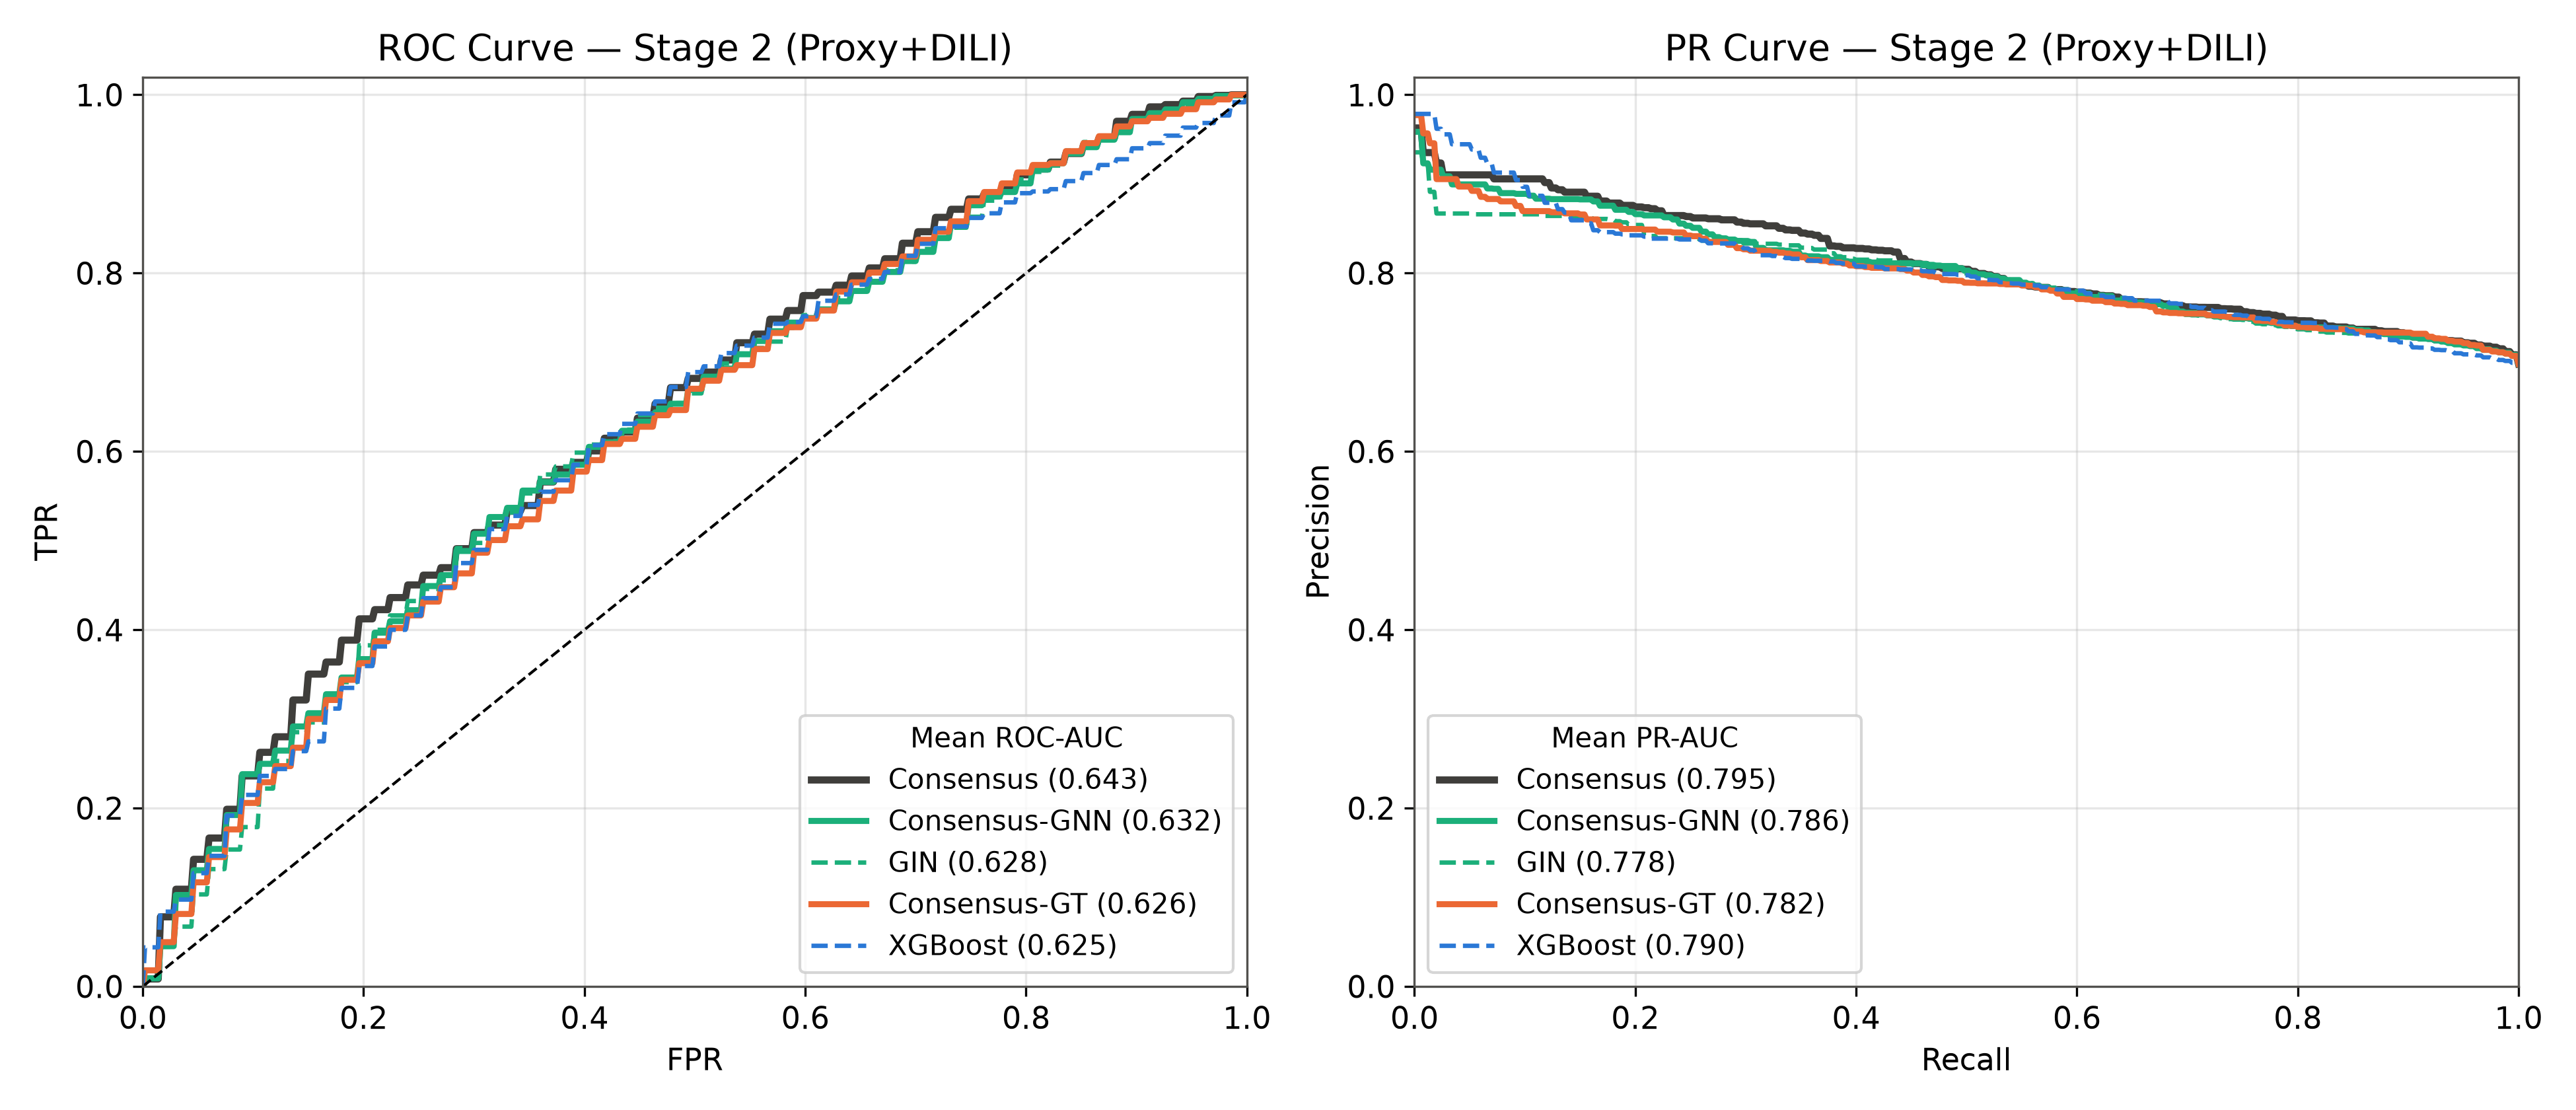
\includegraphics[width=\linewidth]{figures/dili_cv_downsampled_stage2_roc_pr.png}
\caption{ROC (left) and PR (right) curves on the FDA-approved DILI
held-out test set (Held-223; 222 compounds, 155 hepatotoxic/67 non-hepatotoxic)
for the five best Stage~2 (Proxy+DILI) models under 10-fold cross-validation with
a 1:1 downsampled training set.}

    \label{fig:dili_cv_roc_pr}
\end{figure*}

\begin{table*}[t]
\centering
\caption{Performance on the FDA-approved DILI held-out test set (Held-223; 222 compounds, 155 hepatotoxic/67 non-hepatotoxic) -- 10-fold cross-validation, 1:1 downsampled train (mean across 10 folds); Stage 1 (Proxy-only) and Stage 2 (Proxy+DILI); classification cutoff 0.5. Best value per column within each stage in bold.}
\label{tab:dili_cv_downsampled}
\resizebox{\textwidth}{!}{%
\begin{tabular}{lccccccc}
\toprule
\textbf{Model} & \textbf{Sensitivity} & \textbf{Specificity} & \textbf{CCR} & \textbf{ROC-AUC} & \textbf{PR-AUC} & \textbf{MCC} & \textbf{F1} \\
 & (\%) & (\%) & (\%) & & & & \\
\midrule
\multicolumn{8}{c}{\textbf{Stage 1 (Proxy-only)}} \\
\midrule
\multicolumn{8}{l}{\textit{Classical Machine Learning}} \\
\midrule
Random Forest & $59.16 \pm 2.12$ & \underline{$54.78 \pm 6.12$} & $56.97 \pm 2.87$ & $0.596 \pm 0.025$ & $0.770 \pm 0.017$ & $0.129 \pm 0.053$ & $0.662 \pm 0.016$ \\
SVM & $56.96 \pm 2.55$ & $54.02 \pm 4.24$ & $55.50 \pm 2.29$ & $0.576 \pm 0.030$ & $0.738 \pm 0.019$ & $0.101 \pm 0.042$ & $0.644 \pm 0.020$ \\
XGBoost & $53.37 \pm 1.79$ & $53.88 \pm 6.72$ & $53.63 \pm 3.71$ & $0.557 \pm 0.037$ & $0.748 \pm 0.026$ & $0.066 \pm 0.068$ & $0.616 \pm 0.020$ \\
\midrule
\multicolumn{8}{l}{\textit{Graph Neural Networks}} \\
\midrule
GCN & $69.61 \pm 5.70$ & $45.69 \pm 6.44$ & {\boldmath$57.65 \pm 1.17$} & $0.611 \pm 0.015$ & $0.779 \pm 0.013$ & {\boldmath$0.149 \pm 0.022$} & $0.719 \pm 0.029$ \\
GAT & $69.42 \pm 5.99$ & $42.55 \pm 8.90$ & $55.98 \pm 2.72$ & $0.605 \pm 0.025$ & $0.769 \pm 0.021$ & $0.116 \pm 0.051$ & $0.713 \pm 0.030$ \\
GIN & $69.51 \pm 6.03$ & $45.68 \pm 5.53$ & \underline{$57.58 \pm 2.50$} & $0.615 \pm 0.017$ & $0.770 \pm 0.015$ & \underline{$0.148 \pm 0.051$} & $0.719 \pm 0.034$ \\
SAGE & $68.87 \pm 7.76$ & $42.68 \pm 8.17$ & $55.75 \pm 1.77$ & $0.604 \pm 0.021$ & $0.775 \pm 0.016$ & $0.114 \pm 0.034$ & $0.708 \pm 0.042$ \\
\midrule
\multicolumn{8}{l}{\textit{Xu et al. ``Chemical Structure'' model (replicated)}} \\
\midrule
Chemical Structure & $56.51 \pm 2.90$ & {\boldmath$55.07 \pm 5.11$} & $55.80 \pm 2.85$ & $0.583 \pm 0.024$ & $0.764 \pm 0.016$ & $0.107 \pm 0.052$ & $0.642 \pm 0.023$ \\
\midrule
\multicolumn{8}{l}{\textit{Graph Transformers}} \\
\midrule
Graphormer & {\boldmath$73.49 \pm 7.36$} & $38.93 \pm 7.01$ & $56.21 \pm 1.28$ & $0.621 \pm 0.021$ & \underline{$0.783 \pm 0.014$} & $0.128 \pm 0.029$ & \underline{$0.733 \pm 0.038$} \\
GraphGPS & $70.39 \pm 2.67$ & $43.29 \pm 4.85$ & $56.84 \pm 1.45$ & $0.607 \pm 0.026$ & $0.772 \pm 0.024$ & $0.133 \pm 0.027$ & $0.722 \pm 0.012$ \\
\midrule
\multicolumn{8}{l}{\textit{Multi-View GNN }} \\
\midrule
MV-GNN$^{\text{cross}}$ & $63.22 \pm 3.24$ & $48.52 \pm 3.65$ & $55.85 \pm 2.09$ & $0.602 \pm 0.021$ & $0.776 \pm 0.014$ & $0.110 \pm 0.039$ & $0.681 \pm 0.022$ \\
\midrule
\multicolumn{8}{l}{\textit{Consensus Ensembles}} \\
\midrule
Consensus-Classical & $55.48 \pm 2.14$ & $52.85 \pm 6.29$ & $54.16 \pm 3.55$ & $0.580 \pm 0.034$ & $0.756 \pm 0.022$ & $0.077 \pm 0.065$ & $0.631 \pm 0.021$ \\
Consensus-GNN & $69.76 \pm 4.67$ & $44.18 \pm 5.71$ & $56.96 \pm 2.58$ & $0.620 \pm 0.019$ & {\boldmath$0.784 \pm 0.017$} & $0.136 \pm 0.050$ & $0.718 \pm 0.027$ \\
Consensus-GT & \underline{$72.45 \pm 3.30$} & $42.53 \pm 5.38$ & $57.49 \pm 1.88$ & {\boldmath$0.624 \pm 0.017$} & $0.781 \pm 0.016$ & \underline{$0.148 \pm 0.035$} & {\boldmath$0.734 \pm 0.016$} \\
Consensus (Full) & $69.55 \pm 2.00$ & $44.63 \pm 4.38$ & $57.09 \pm 2.28$ & \underline{$0.622 \pm 0.025$} & {\boldmath$0.784 \pm 0.015$} & $0.137 \pm 0.043$ & $0.719 \pm 0.014$ \\
\midrule
\multicolumn{8}{c}{\textbf{Stage 2 (Proxy+DILI)}} \\
\midrule
\multicolumn{8}{l}{\textit{Classical Machine Learning}} \\
\midrule
Random Forest & $61.63 \pm 2.13$ & $51.80 \pm 4.12$ & $56.70 \pm 2.01$ & $0.606 \pm 0.020$ & $0.780 \pm 0.012$ & $0.125 \pm 0.037$ & $0.675 \pm 0.015$ \\
SVM & $62.00 \pm 1.88$ & $49.11 \pm 6.27$ & $55.56 \pm 2.99$ & $0.594 \pm 0.032$ & $0.749 \pm 0.024$ & $0.103 \pm 0.055$ & $0.674 \pm 0.014$ \\
XGBoost & $63.75 \pm 2.07$ & {\boldmath$55.97 \pm 5.09$} & {\boldmath$59.85 \pm 2.80$} & $0.625 \pm 0.039$ & \underline{$0.790 \pm 0.027$} & {\boldmath$0.183 \pm 0.052$} & $0.697 \pm 0.017$ \\
\midrule
\multicolumn{8}{l}{\textit{Graph Neural Networks}} \\
\midrule
GCN & {\boldmath$71.04 \pm 5.88$} & $44.03 \pm 6.58$ & $57.53 \pm 1.81$ & $0.623 \pm 0.018$ & $0.780 \pm 0.014$ & $0.148 \pm 0.036$ & \underline{$0.726 \pm 0.031$} \\
GAT & $69.60 \pm 3.36$ & $45.38 \pm 5.56$ & $57.48 \pm 2.46$ & $0.610 \pm 0.024$ & $0.769 \pm 0.020$ & $0.144 \pm 0.047$ & $0.720 \pm 0.020$ \\
GIN & $66.91 \pm 6.25$ & $51.65 \pm 7.55$ & $59.27 \pm 1.87$ & $0.628 \pm 0.022$ & $0.778 \pm 0.021$ & $0.177 \pm 0.034$ & $0.710 \pm 0.034$ \\
SAGE & $64.20 \pm 7.02$ & $50.46 \pm 9.23$ & $57.33 \pm 2.70$ & $0.610 \pm 0.021$ & $0.774 \pm 0.020$ & $0.139 \pm 0.050$ & $0.689 \pm 0.039$ \\
\midrule
\multicolumn{8}{l}{\textit{Xu et al. ``Chemical Structure'' model (replicated)}} \\
\midrule
Chemical Structure & $62.00 \pm 2.38$ & $51.20 \pm 5.35$ & $56.59 \pm 2.00$ & $0.598 \pm 0.020$ & $0.767 \pm 0.015$ & $0.123 \pm 0.036$ & $0.677 \pm 0.012$ \\
\midrule
\multicolumn{8}{l}{\textit{Graph Transformers}} \\
\midrule
Graphormer & $70.00 \pm 5.69$ & $43.28 \pm 7.28$ & $56.64 \pm 1.55$ & $0.616 \pm 0.017$ & $0.779 \pm 0.010$ & $0.130 \pm 0.029$ & $0.718 \pm 0.029$ \\
GraphGPS & $70.32 \pm 2.82$ & $43.30 \pm 4.07$ & $56.78 \pm 2.64$ & $0.607 \pm 0.029$ & $0.770 \pm 0.020$ & $0.132 \pm 0.052$ & $0.722 \pm 0.020$ \\
\midrule
\multicolumn{8}{l}{\textit{Multi-View GNN }} \\
\midrule
MV-GNN$^{\text{cross}}$ & $61.35 \pm 6.46$ & $48.07 \pm 5.66$ & $54.72 \pm 2.12$ & $0.601 \pm 0.022$ & $0.776 \pm 0.017$ & $0.089 \pm 0.040$ & $0.665 \pm 0.043$ \\
\midrule
\multicolumn{8}{l}{\textit{Consensus Ensembles}} \\
\midrule
Consensus-Classical & $64.07 \pm 2.34$ & \underline{$53.30 \pm 4.93$} & $58.66 \pm 2.23$ & $0.620 \pm 0.032$ & $0.779 \pm 0.021$ & $0.162 \pm 0.041$ & $0.695 \pm 0.015$ \\
Consensus-GNN & $67.93 \pm 3.53$ & $48.52 \pm 5.04$ & $58.22 \pm 1.92$ & \underline{$0.631 \pm 0.020$} & $0.786 \pm 0.015$ & $0.157 \pm 0.036$ & $0.714 \pm 0.020$ \\
Consensus-GT & \underline{$70.56 \pm 3.28$} & $44.33 \pm 4.01$ & $57.45 \pm 2.14$ & $0.626 \pm 0.020$ & $0.782 \pm 0.015$ & $0.145 \pm 0.043$ & $0.725 \pm 0.020$ \\
Consensus (Full) & $70.46 \pm 3.00$ & $48.51 \pm 5.55$ & \underline{$59.47 \pm 2.78$} & {\boldmath$0.643 \pm 0.020$} & {\boldmath$0.795 \pm 0.013$} & \underline{$0.182 \pm 0.052$} & {\boldmath$0.731 \pm 0.020$} \\
\bottomrule
\end{tabular}%
}
\end{table*}


\FloatBarrier

% \begin{figure}
%     \includegraphics[width=\linewidth]{figures/liver_all_proxy_dili_f1_roc.png}
%     \caption{F1 and ROC-AUC scores for all models under the Proxy+DILI
%     setting on the FDA DILI held-out test set. Graph-based model names
%     are highlighted in red.}
%     \label{fig:liver_bar}
% \end{figure}

\begin{figure*}[h]
    \centering
    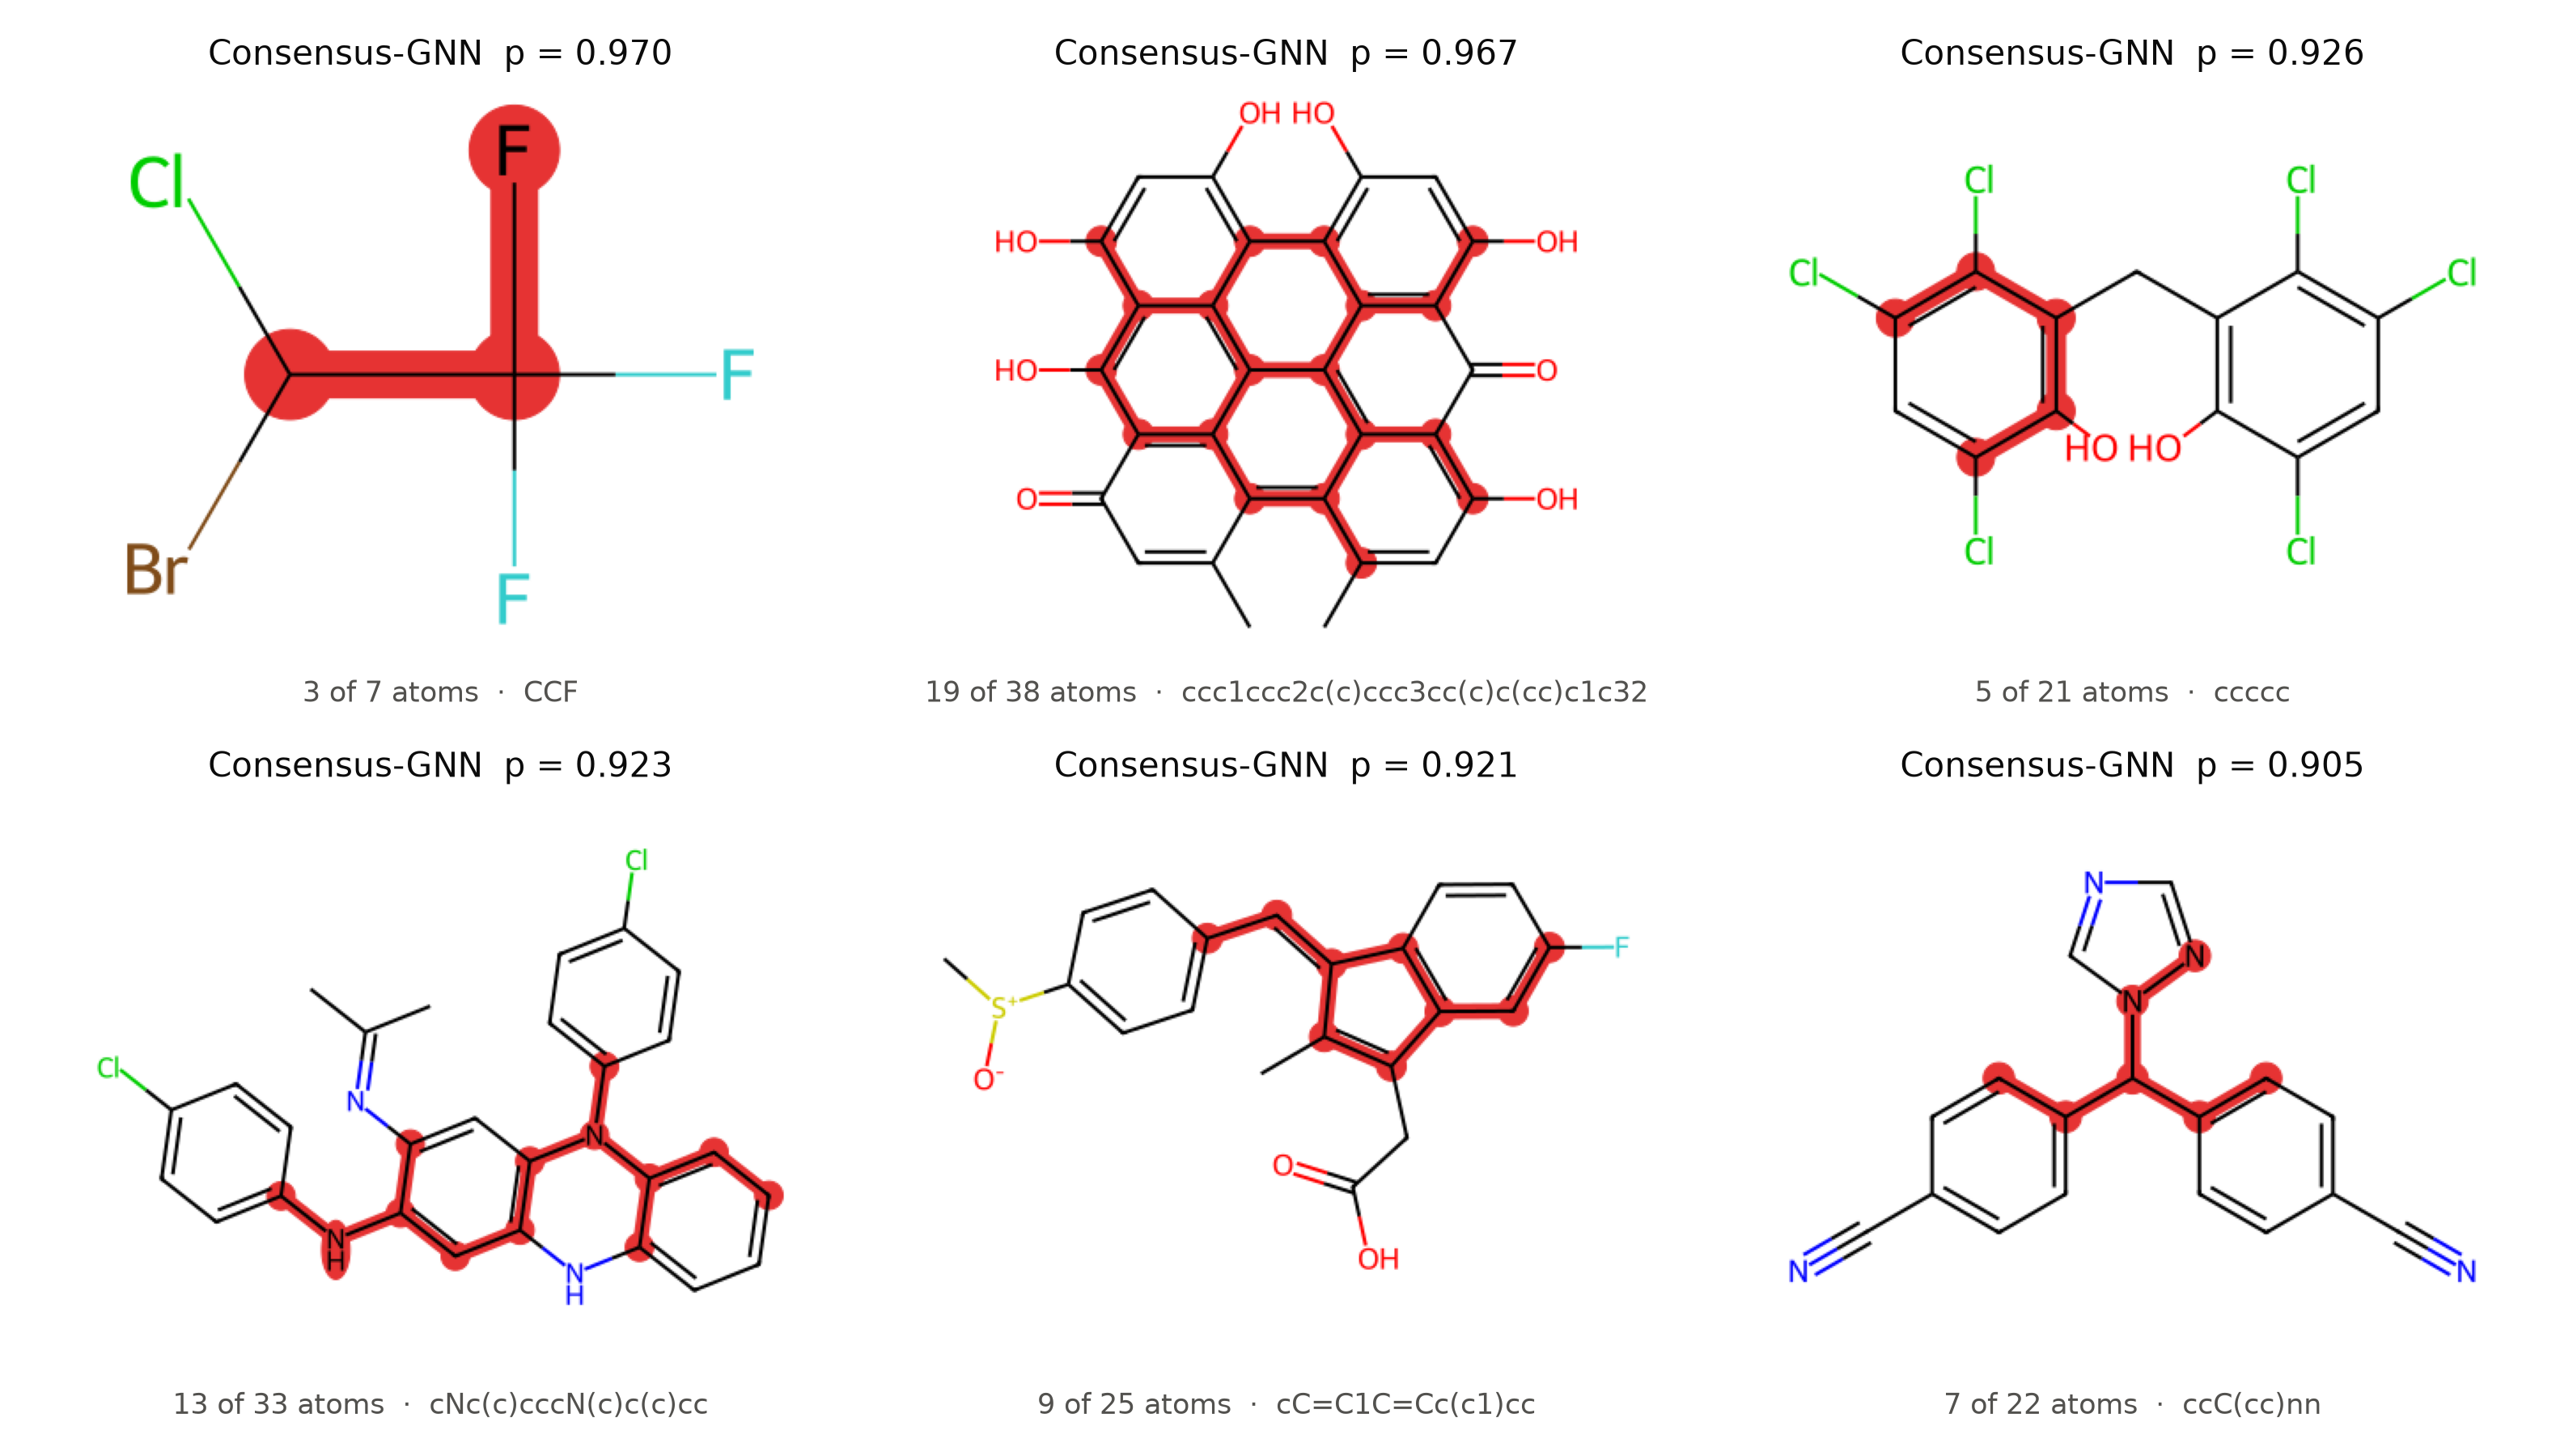
\includegraphics[width=\linewidth]{figures/subgraphx_consensus_gnn.png}
    \caption{Consensus DILI compounds flagged by Consensus-GNN (GCN, GAT, GIN and
    GraphSAGE). Red subgraphs highlight the toxic structural motifs; the consensus
    confidence score, the mean of the four models, is shown above each compound.}
    \label{fig:xai_consensus}
\end{figure*}

\FloatBarrier

\textbf{Table~\ref{tab:dili_cv_downsampled}} reports the performance under the cross-validation split, downsampled training for all tested models on the 222-compound FDA DILI held-out test set in the Proxy-only and Proxy+DILI stages. The full consensus achieved the best overall performance (ROC-AUC 0.643, F1 0.731), followed by Consensus-GNN (0.631, 0.714), Consensus-GT (0.626, 0.725) and then Consensus-Classic (0.62, 0.695). For individual models, several models achieved decent performance of ROC-AUC at least 0.62, including GIN, GCN, XGBoost, and Graphormer in the Proxy+DILI setting. Interestingly, Graphormer recorded even better performance of ROC-AUC 0.621 and F1 0.733 in the Proxy-only setting, which drop slightly to 0.616 and 0.718. In fact, involving DILI training data improves each of the GNNs and classic models, often by ROC-AUC 0.01 and up to 0.07. However, the two graph transformers and multi-view GNN got the same or slightly decreased performance, possibly because their generally robust capabilities already learn useful information in the Proxy-only setting.

In the repeated random split, the relative position of the consensus ensembles remains similar, where the full consensus achieved ROC-AUC 0.634 and F1 0.735, followed by Consensus-GT (0.623, 0.726), Consensus-GNN (0.622, 0.719), and Consensus-Classic (0.615, 0.688). Remarkably, Graphormer obtained competitive performance both in the Proxy-only setting (0.629, 0.748) and in the Proxy-DILI setting (0.625, 0.752). In the scaffold split, classic machine learning models appear to suffer, where Consensus-Classic recorded only ROC-AUC at 0.601, smaller than Consesus-GNN by 0.02. GCN achieved robust performance of ROC-AUC 0.636 and F1 0.748.

% \textbf{Table~\ref{tab:dili_random_up_assay_style}} reports repeated
% random-split performance with up-sampled training for all fifteen entries on
% the 222-compound FDA DILI held-out test set, for the Proxy-only and
% Proxy+DILI stages. Fine-tuning on the DILI training data improved ROC-AUC for
% fourteen of the fifteen, the exception being Graphormer, which declined from
% 0.603 to 0.591; the benefit of DILI fine-tuning is therefore
% architecture-dependent rather than universal. The gains are largest for the
% classical models, which start furthest behind (XGBoost 0.587 to 0.631, SVM
% 0.590 to 0.613), and smaller for the graph neural networks, which already
% perform well under Proxy-only (GCN 0.635 to 0.641, GIN 0.623 to 0.628). At
% the 0.50 cutoff the full consensus achieved the best ROC-AUC (0.644), CCR
% (61.7\%) and MCC (0.215) in the Proxy+DILI stage, with GCN second on ROC-AUC
% (0.641) and best on F1 (0.712). XGBoost gives the best PR-AUC (0.800),
% although PR-AUC is of limited use on this test set.

% Graph-based architectures account for the strongest individual models in both
% stages. Under Proxy-only, GCN leads every model on ROC-AUC (0.635) and PR-AUC
% (0.793), ahead of Consensus-GNN (0.628) and GIN (0.623), while the best
% classical model, Random Forest, reaches 0.612. Under Proxy+DILI the four
% message-passing networks occupy three of the four highest individual ROC-AUC
% values. The family-specific ensembles do not consistently improve on their own
% best constituent here: Consensus-Classical (0.629) falls below XGBoost
% (0.631) and Consensus-GNN (0.635) below GCN (0.641), whereas Consensus-GT
% (0.617) exceeds both graph transformers. Only the full consensus exceeds every
% individual model, suggesting that on this small, structurally diverse
% benchmark combining all three architecture families is more beneficial than
% combining within a single family.

% \textbf{Figure~\ref{fig:dili_scaffold}} shows the same models under the
% repeated scaffold split, where the test compounds carry scaffolds not seen
% during training. The separation by architecture is clearer in this harder
% setting. Under Proxy-only the seven graph-based models occupy the top seven
% positions among individual models, led by Graphormer (0.622), with the three
% classical models last (Random Forest 0.570, XGBoost 0.560, SVM 0.554). Under
% Proxy+DILI, GCN leads (0.625) ahead of GIN (0.620) and Graphormer (0.614).
% Absolute performance is lower than on the random split for every model, as
% expected, and the margin between the best graph model and the best classical
% model widens from 0.023 to 0.052 ROC-AUC under Proxy-only. GraphGPS is the
% exception among the graph models, falling to the bottom of the ranking under
% Proxy+DILI (0.565).

Two external baselines were evaluated on the same splits. MV-GNN$^{cross}$, a
multi-view message-passing architecture excluded from all consensus
ensembles, reaches 0.593 under Proxy+DILI on the random split and 0.592 under
the scaffold split, below the full consensus in both. The replicated
chemical-structure workflow of Xu~\textit{et al.}, which uses ECFP4
fingerprints with Random-Forest feature selection and an SVM classifier,
reaches 0.609 and 0.591 respectively, below every consensus ensemble and below
GIN in both settings.

\textbf{Figure~\ref{fig:xai_consensus}}
presents SubgraphX explanations for the top-6 consensus true positives on the FDA-approved DILI held-out test set. SubgraphX~\cite{yuan2021subgraphx} identifies the minimal connected subgraph most responsible for the model's prediction; highlighted atoms (red) represent the structural alert driving the hepatotoxic classification. The consensus panel shows the top-6 of the 99 compounds flagged by Consensus-GNN, led by halothane (prob=0.970) and hexachlorophene (prob=0.926), where agreement across the four GNNs on known hepatotoxins suggests the models have learned chemically meaningful structural alerts. The number of six compounds was chosen only to keep the figure readable within the available page space.

Our proposed graph-based QSAR modeling pipeline, using only molecular graph
structure, exceeded the previously best model, the multi-feature
DILIPredictor \cite{seal2024} (ROC-AUC 0.63, F1 0.65 on the \emph{same}
held-out test set), which additionally incorporated physicochemical
descriptors and pharmacokinetic parameters; our full consensus model reached a
ROC-AUC of 0.644 and GCN an F1 of 0.712 (Proxy+DILI, repeated random split,
0.50 cutoff). Based on these results, we will further explore how to leverage
abundant existing hepatotoxicity studies from PubMed literature and use
advanced LLM-driven approaches for improving DILI prediction of novel
compounds.


% Transfer-learning GNNs demonstrated consistent improvement with NCV-888 augmentation:
% TL-GAT-aug reached the highest sensitivity among GNNs at 67.7\%, with an F1 of 0.727.
% Graph transformer models benefit substantially from the two-stage DILI pretraining strategy. Graphormer-aug achieved a very high sensitivity of 85.8\% with an F1 of 0.799, reflecting a recall-biased decision boundary, while GraphGPS-aug exhibited the complementary pattern (specificity 82.1\%, sensitivity 36.8\%).
% This divergence reflects the different inductive biases of both architectures and motivated combining them within the six-way consensus.

% The six-way consensus ensemble (RF-aug + XGB-aug + TL-GIN + TL-GAT-aug + Graphormer-aug + GraphGPS-aug) achieved the best ROC-AUC of \textbf{0.6979}, CCR of 66.5\%, and MCC of 0.305, with a balanced sensitivity/specificity of 65.8\%/67.2\% and F1 of 0.731.
% Notably, the logistic-regression stacking meta-learner performed below the simple consensus average (ROC-AUC 0.659 vs.\ 0.692), consistent with the small training set limiting the meta-learner's ability to learn reliable model weights.
% This demonstrates that molecular graph representations combined with transfer learning
% and consensus aggregation are sufficient to exceed multi-feature baselines on this clinically challenging hepatotoxicity benchmark.

\subsection{Cytotoxicity Induction Behavior and Structural Analysis}
\subsubsection{Mitochondrial Membrane Potential (MMP) Disruption Pathway and Caspase-3/7 Activation}

Since both Caspase-3/7 activation and MMP disruption data are available in HepG2 cells, this enables pairwise comparison between compounds tested in both assays to identify activation patterns and analyze the underlying apoptosis pathway. As shown in \textbf{Table~\ref{tab:caspase_mito}}, 106 of 4,879 compounds (2.2\%) were active in both Caspase and mitochondrial summary assays, consistent with the mitochondrial pathway leading to apoptosis. Twenty compounds (0.4\%) were Caspase-active but mitochondria-inactive. Compared with the 2.2\% dual-active category, this indicates a majority of the Caspase activation is associated with mitochondrial activity. Because the two assays were measured independently and at a single time point, this association does not establish causality or temporal ordering, though it is consistent with the general understanding on the mitochondrial pathway to apoptosis.  We now analyze representative substructures presented in "both active" compounds vs "both inactive" compounds in Table~\ref{tab:caspase_mito}.


\begin{table}[t]
\centering
\small
\caption{Pairwise comparison of Caspase-3/7 and mitochondrial activity in
HepG2 cells, using the summary assays}
\label{tab:caspase_mito}
\begin{tabular}{lc}
\hline
\textbf{Category} & \textbf{Count} \\
\hline
Both active                           & 106 (2.2\%)     \\
Caspase active, mitochondria inactive & 20 (0.4\%)      \\
% Caspase inactive, mitochondria active & 511 (10.5\%)  \\
Both inactive                         & 4{,}242 (86.9\%)\\
\hline
% \textbf{Total} & \textbf{4{,}879} \\
% \hline
\end{tabular}
\end{table}

%table 4 caspase +mito hepg2 
\paragraph{Structural Motifs in Dual-Active Versus Dual-Inactive Compounds.}

\begin{figure*}[h!]
\centering
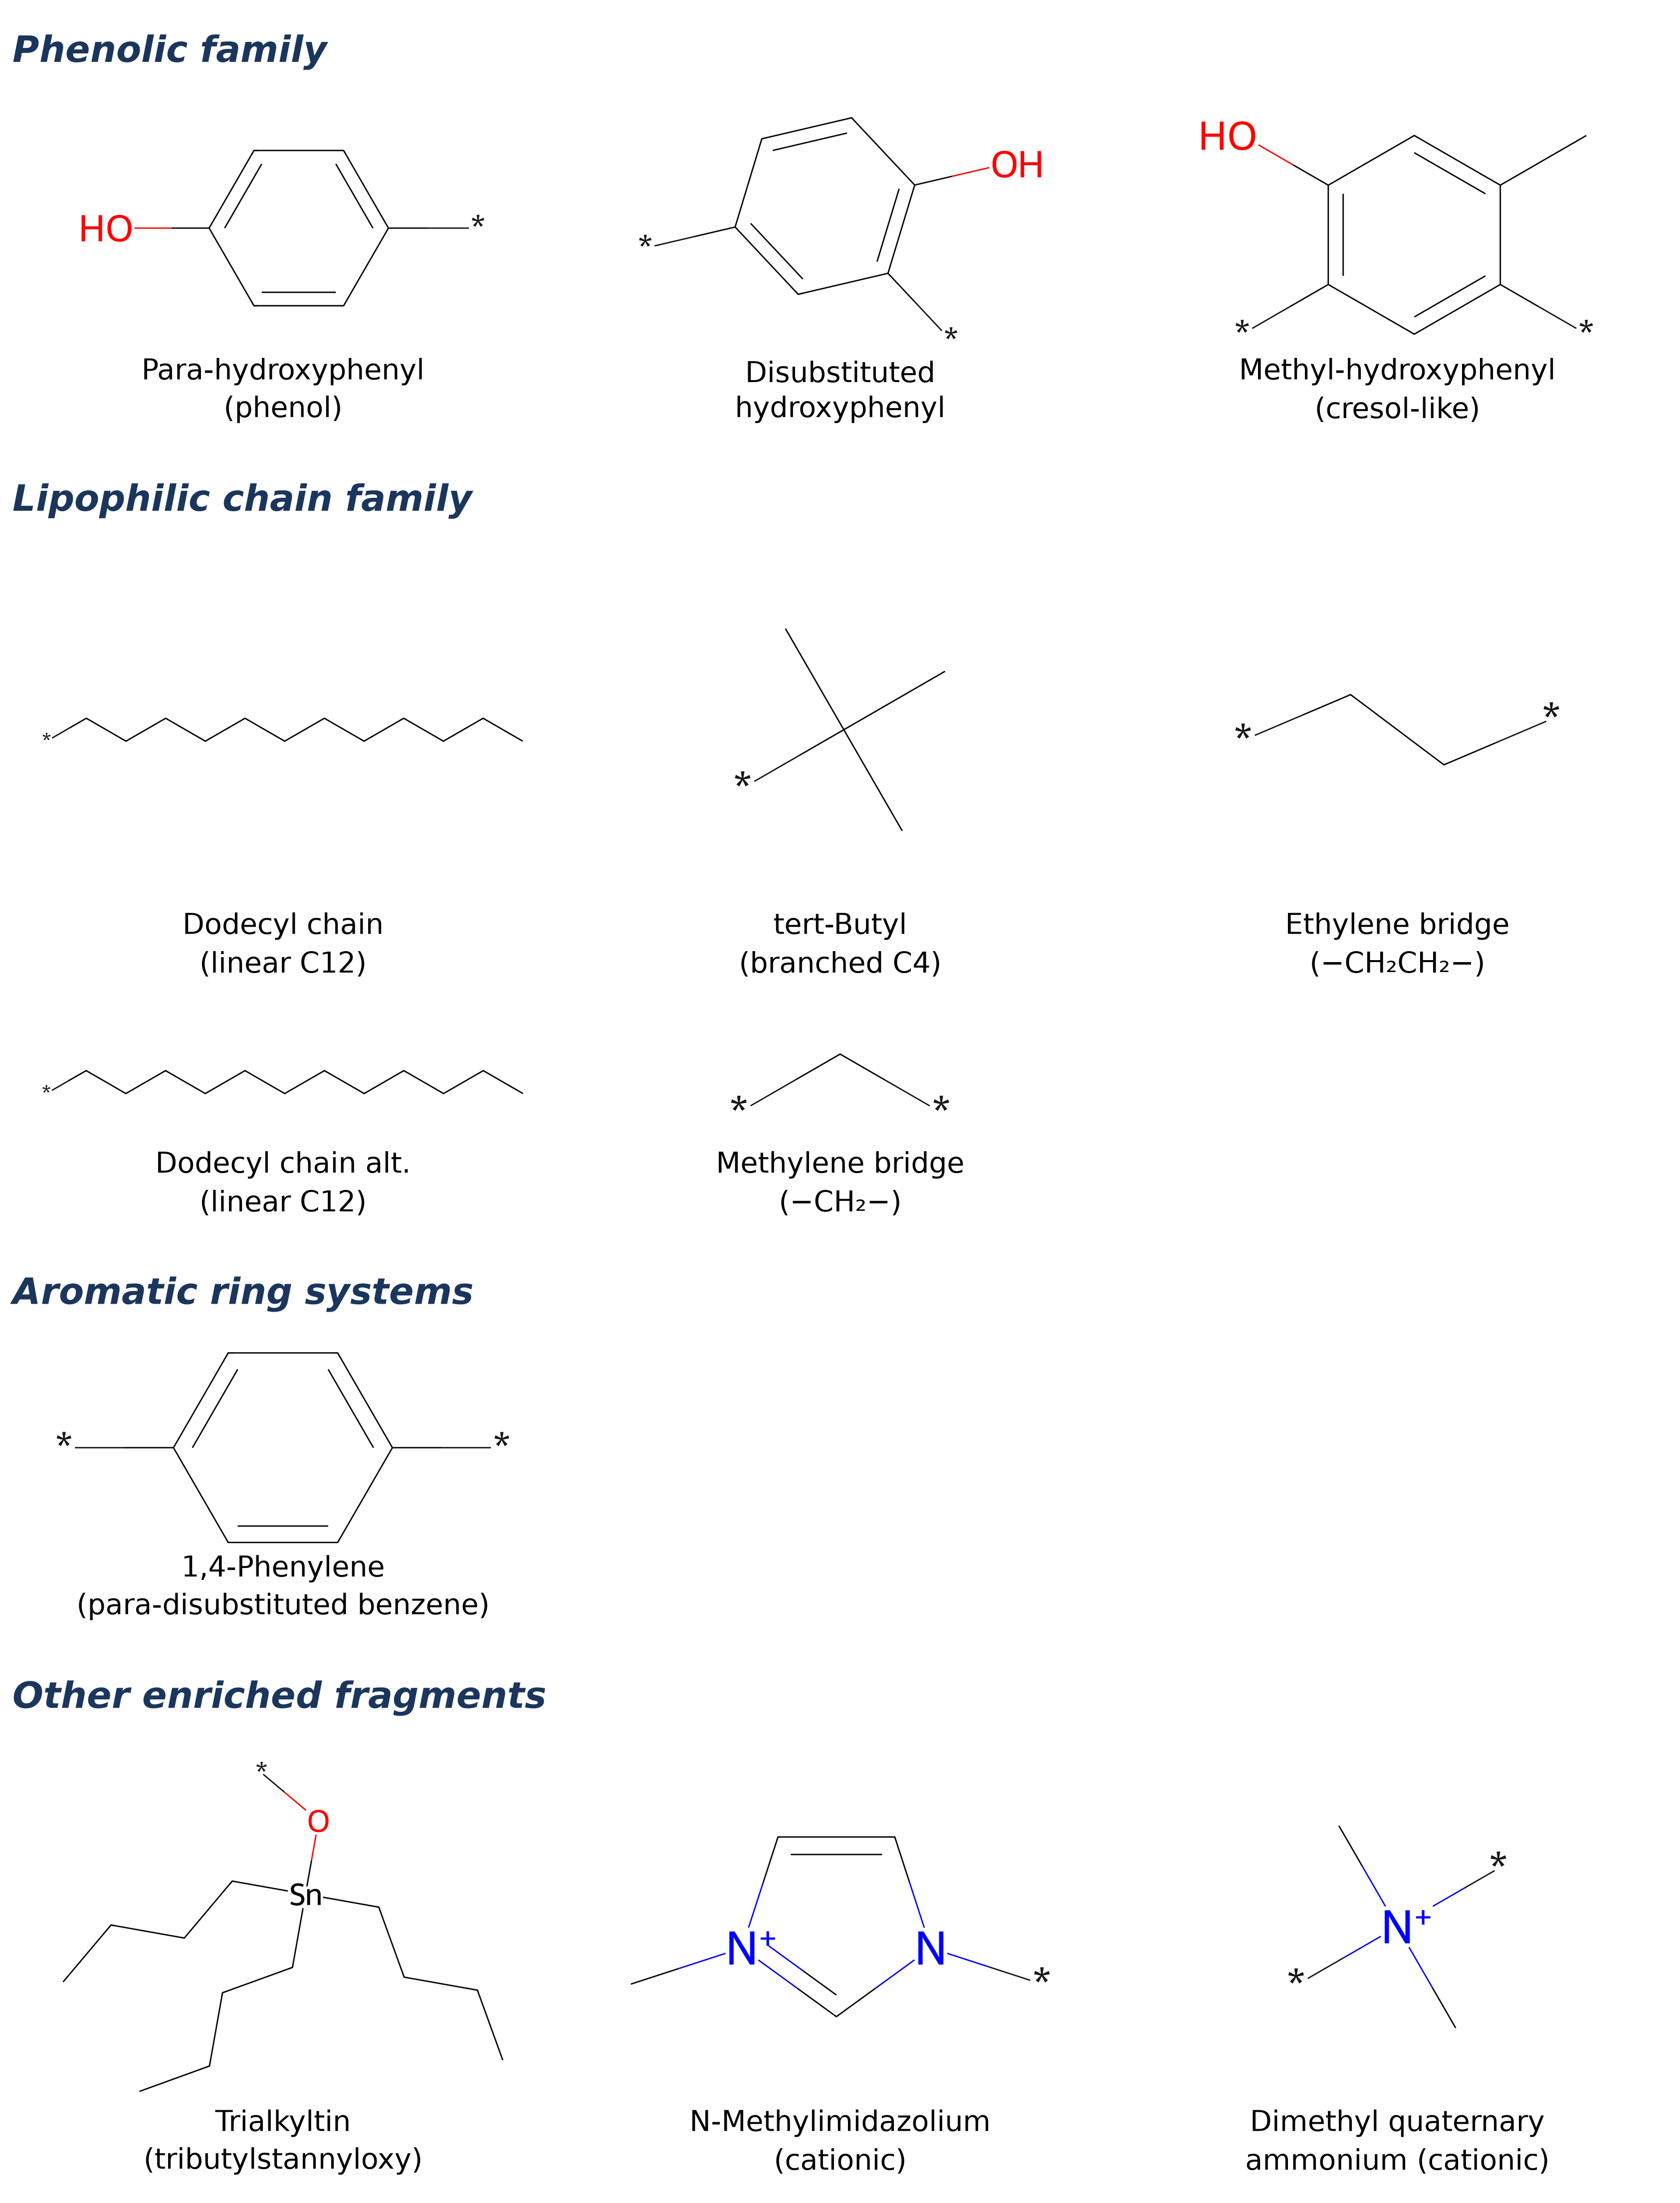
\includegraphics[width=0.8\linewidth]{figures/fig_brics_enriched_fragments.png}
\caption{%
    All 12 BRICS fragments significantly enriched in \textbf{dual-active} (Caspase $+$ mitochondrial) versus dual-inactive compounds,
    grouped by the structural family. BRICS attachment points are drawn as $*$; each fragment is
    scaled individually for legibility, so sizes are not comparable across panels. Full enrichment statistics, including
    odds ratios, adjusted $p$-values, and per-group prevalence counts,
    are provided in Table~\ref{tab:brics_strict_enrichment}.%
}
\label{fig:brics_enriched_fragments}
\end{figure*}

\begin{table*}[h!]
\centering
\small
\caption{%
    All 12 BRICS fragments significantly enriched in dual-active
    (Caspase $+$ mitochondrial) versus dual-inactive compounds
    ($n_{\text{active}} = 106$, $n_{\text{inactive}} = 4{,}242$),
    grouped by structural family and ranked by adjusted $p$-value
    (Benjamini--Hochberg, $\alpha = 0.05$).
    OR~$= \infty$ denotes fragments absent from the dual-inactive set. \% active and \% inactive denote percentages of dual-active and dual-inactive compounds with a fragment respectively.
    The two dodecyl entries are the same C12 chain recovered through different BRICS bond types.
}
\label{tab:brics_strict_enrichment}
\begin{tabular}{lp{2.6cm}ccc}
\hline
\textbf{Fragment name} &
\textbf{Structure} &
\textbf{OR} &
\textbf{$p_{\text{adj}}$} &
\textbf{\% active vs \% inactive} \\
\hline
\multicolumn{5}{l}{\textit{Phenolic family}} \\[2pt]
Para-hydroxyphenyl (phenol) &
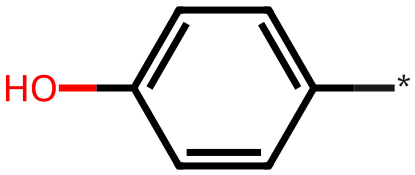
\includegraphics[width=1cm,keepaspectratio]{figures/frag_phenol.png} &
18.8 & $7.0\times10^{-9}$ & 10.38\% vs 0.61\% \\[8pt]
Disubstituted hydroxyphenyl &
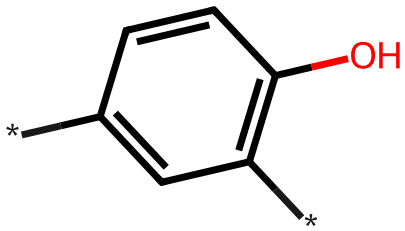
\includegraphics[width=1cm,keepaspectratio]{figures/frag_hydroxyphenyl.png} &
37.4 & $2.0\times10^{-7}$ & 6.60\% vs 0.19\% \\[8pt]
Methyl-hydroxyphenyl (cresol-like) &
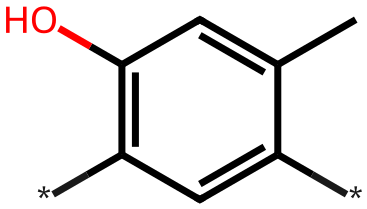
\includegraphics[width=1cm,keepaspectratio]{figures/frag_methylhydroxyphenyl.png} &
$\infty$ & $7.3\times10^{-5}$ & 2.83\% vs 0\% \\[8pt]
\hline
\multicolumn{5}{l}{\textit{Lipophilic chain family}} \\[2pt]
Dodecyl chain (linear C12) &
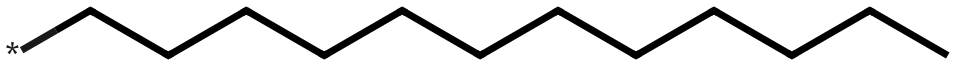
\includegraphics[width=1.6cm,keepaspectratio]{figures/frag_dodecyl.png} &
99.9 & $7.0\times10^{-9}$ & 6.60\% vs 0.07\% \\[8pt]
\textit{tert}-Butyl (branched C4) &
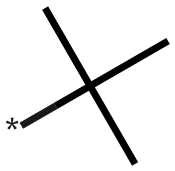
\includegraphics[width=0.9cm,keepaspectratio]{figures/frag_tertbutyl.png} &
7.2 & $3.8\times10^{-3}$ & 4.72\% vs 0.68\% \\[8pt]
Ethylene bridge ($-$CH$_2$CH$_2$$-$) &

\includegraphics[width=0.9cm,keepaspectratio]{figures/frag_ethylene.png} &
11.2 & $1.1\times10^{-2}$ & 2.83\% vs 0.26\% \\[8pt]
Dodecyl chain, alt.\ (linear C12) &
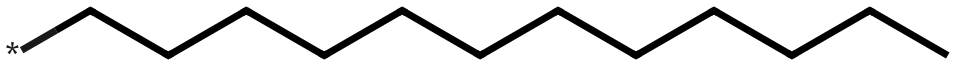
\includegraphics[width=1.6cm,keepaspectratio]{figures/frag_dodecyl_alt.png} &
8.8 & $1.8\times10^{-2}$ & 2.83\% vs 0.33\% \\[8pt]
Methylene bridge ($-$CH$_2$$-$) &
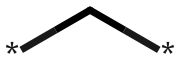
\includegraphics[width=0.9cm,keepaspectratio]{figures/frag_methylene.png} &
3.9 & $2.8\times10^{-2}$ & 4.72\% vs 1.25\% \\[8pt]
\hline
\multicolumn{5}{l}{\textit{Aromatic ring systems}} \\[2pt]
1,4-Phenylene (para-disubstituted benzene) &
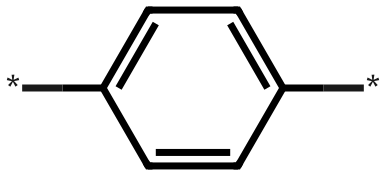
\includegraphics[width=1.2cm,keepaspectratio]{figures/frag_phenylene.png} &
3.3 & $3.8\times10^{-3}$ & 10.38\% vs 3.42\% \\[8pt]
\hline
\multicolumn{5}{l}{\textit{Other enriched fragments}} \\[2pt]
Trialkyltin (tributylstannyloxy) &
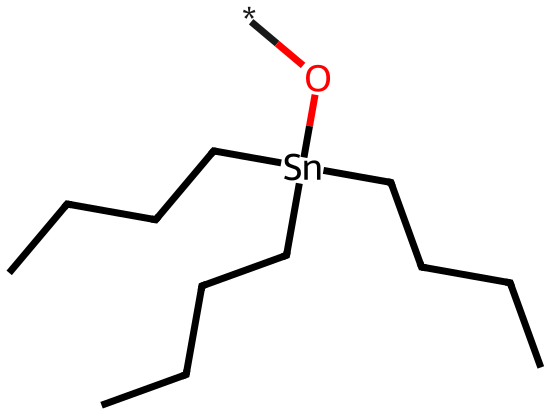
\includegraphics[width=1.2cm,keepaspectratio]{figures/frag_organotin.png} &
$\infty$ & $7.3\times10^{-5}$ & 2.83\% vs 0\% \\[8pt]
\textit{N}-Methylimidazolium (cationic) &
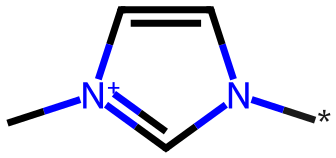
\includegraphics[width=1.1cm,keepaspectratio]{figures/frag_imidazolium.png} &
7.9 & $1.2\times10^{-3}$ & 5.66\% vs 0.75\% \\[8pt]
Dimethyl quaternary ammonium (cationic) &
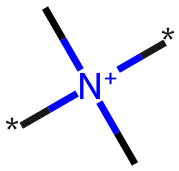
\includegraphics[width=0.9cm,keepaspectratio]{figures/frag_ammonium.png} &
24.7 & $2.7\times10^{-3}$ & 2.83\% vs 0.12\% \\[8pt] \hline
\end{tabular}
\end{table*}

To identify structural features associated with compounds that fully engage
the caspase--mitochondrial apoptotic cascade, a \emph{Breaking Retrosynthetically Interesting Chemical Substructures (BRICS)} fragment enrichment
analysis was performed contrasting 106 dual-active compounds against 4{,}242
dual-inactive compounds, both drawn from the HepG2 summary assays. Specifically, the BRICS method \cite{degen2008art} first decomposes these compounds into chemically meaningful fragments. Then a one-sided Fisher's exact test with Benjamini--Hochberg correction ($\alpha = 0.05$) is applied to each fragment to decide whether it is significantly presented in dual-active compared to dual-inactive compounds. The one-sided Fisher's exact test was chosen because fragment occurrence is binary per molecule and expected cell counts are frequently below five in targeted chemical subsets, making the chi-squared approximation unreliable; the one-sided formulation tests the directional hypothesis that a fragment appears more often in actives than inactives. This analysis identified 12 significantly enriched fragments in the dual-active foreground compared to the dual-inactive background
(\textbf{Figure~\ref{fig:brics_enriched_fragments};
Table~\ref{tab:brics_strict_enrichment}}), which can be organized into
four structural families. These fragments characterise a substantial subset of the
foreground rather than the whole of it: 49 of the 106 dual-active compounds (46.2\%)
carry at least one of them, so they are enriched markers of dual activity rather than
a complete structural description of it.

The \emph{phenolic} family comprised three fragments and produced the strongest
signal. A para-hydroxyphenyl motif was among the top-ranked fragments overall, that is the ones with smallest adjusted $p$-value
($p_{\text{adj}} = 7.0 \times 10^{-9}$, shared with the dodecyl chain). It is presented in 10.4\% of
dual-active compounds versus 0.6\% of dual-inactive compounds, the broadest
foreground support of any fragment in the set. A
disubstituted hydroxyphenyl variant and a methyl-hydroxyphenyl (cresol-like)
motif in the phenolic family further
reinforced this finding. Together, these fragments establish
hydroxyl-substituted aromatic rings as the most statistically reliable
structural predictor of caspase--mitochondrial co-activation.

% [CORRECTED] the old draft attributed the methylene bridge and the second
% dodecyl variant to "branched connectivity"; neither fragment is branched.
The \emph{lipophilic chain} family comprised five fragments, including branched and
linear alkyl fragments from one- and two-carbon bridges up to C12. The linear C12
chain (dodecyl) showed the strongest enrichment within this
group ($p_{\text{adj}} = 7.0 \times 10^{-9}$, OR $= 99.9$), followed by \textit{tert}-butyl and an ethylene bridge. A methylene bridge and a second dodecyl variant, recovered through a different BRICS bond type, were also enriched, reflecting the short linear linkers and quaternary carbon centres
typical of this compound class.

% [CORRECTED] the previous draft claimed the phenolic and lipophilic families
% represent "two structurally independent routes". They are positively
% associated (OR = 4.15, two-sided Fisher p = 0.013), so "independent" is wrong.
Twenty-one dual-active compounds carry a phenolic fragment and twenty-two carry a
lipophilic-chain fragment, of which nine carry both. The two families therefore
describe at least two distinct structural routes to dual apoptotic activity, but they
are not independent of one another: their co-occurrence is greater than expected by
chance (OR $= 4.15$, two-sided Fisher's exact $p = 0.013$), driven largely by
hindered phenols that carry \textit{tert}-butyl substituents on the phenol ring and by
alkylphenols that combine a C12 chain with a para-hydroxyphenyl group in a single
molecule.

The \emph{aromatic ring system} family comprised a single fragment, a
1,4-phenylene (para-disubstituted benzene) motif ($p_{\text{adj}} = 3.8 \times 10^{-3}$);
its modest odds ratio (3.3) and its 3.4\% prevalence among dual-inactive
compounds indicate a generic linker rather than a specific pharmacophore.
The remaining three enriched fragments spanned distinct chemical classes: a
\emph{trialkyltin group}, an \emph{\textit{N}-methylimidazolium cation}, and a
\emph{dimethyl quaternary ammonium cation}. Two fragments were identified
exclusively in dual-active compounds (and not presented in dual-inactive
compounds): the trialkyltin group and the methyl-hydroxyphenyl motif of the
phenolic family (both with $p_{\text{adj}} = 7.3 \times 10^{-5}$).
% [CORRECTED] the previous draft read the reverse-direction null as proof that
% inactivity has no motif. A null result does not establish absence, so the
% claim is now stated as the null it is.
It should be noted that the reverse analysis---fragments enriched in dual-inactive
compounds compared to dual-active compounds---returned no significant hits at any
occurrence threshold tested, so no common fragment was found to be depleted in the
dual-active set; this is a negative result and does not by itself establish that
structural inactivity lacks a defining chemical motif.


Compounds featuring lipophilic alkyl chains and cationic groups, such as delocalized lipophilic cations, were reported to selectively accumulate within mitochondria due to the negative potential characteristic of the mitochondrial inner membrane; here, they can directly interfere with mitochondrial function \cite{dzajic2025lipophilic}. Notably, enhancing lipophilicity through the introduction of longer alkyl chains increases a compound's affinity for membranes as well as the extent of its accumulation within mitochondria. This heightened lipophilicity correlates positively with the compound's capacity to reduce the mitochondrial inner membrane potential ($\Delta \psi_m$); the underlying mechanism involves disrupting the integrity of the inner mitochondrial membrane and increasing proton leakage \cite{trnka2015lipophilic}. These lipophilic cationic compounds can intercalate into mitochondrial membranes, disrupt the function of respiratory chain complexes, and ultimately trigger the collapse of $\Delta \psi_m$ \cite{trnka2015lipophilic}, leading to the activation of caspases-3 and -7. Furthermore, phenolic groups and redox-active moieties can also induce mitochondrial dysfunction and thereby further destabilize the membrane potential by promoting oxidative stress and mitochondrial damage \cite{fernandes2021cytotoxicity}. This study's enrichment analysis associates phenolic compounds bearing a  para-hydroxyphenyl motif, as well as members of the lipophilic chain family specifically those possessing structural amphiphilicity (combining hydrophobic and polar characteristics) or ionophore-like structures, with disruption of the ion gradients across the mitochondrial membrane. Consistent with this description, the C12 chain co-occurs with an \textit{N}-methylimidazolium head group in four dual-active compounds and with a dimethyl quaternary ammonium head group in two, so that chain and cation are carried by the same molecules and together constitute delocalized lipophilic cations. This association is consistent with a mechanism in which such disruption contributes to dissipating $\Delta \psi_m$ and to mitochondrial swelling and dysfunction, though our data are associative and do not themselves establish this causal pathway. In contrast, compounds lacking sufficient lipophilicity or specific mitochondrial-targeting features exhibit lower levels of mitochondrial accumulation and, consequently, exert a relatively weaker disruptive effect on $\Delta \psi_m$.
Moreover, amine-containing groups, such as the dimethyl quaternary ammonium and \textit{N}-methylimidazolium cations identified here, when permanently charged or integrated into an ionizable molecular scaffold, can influence a compound's mitochondrial-targeting behavior by modulating the balance between membrane permeability and charge-driven accumulation. Relevant experimental studies utilizing lipophilic cations coupled with ionizable groups (including amino groups) have demonstrated that the efficiency of compound uptake within mitochondria depends on the compound's $pK_a$ value, its protonation state, and the pH gradient across the mitochondrial membrane; this directly confirms that amino functional groups play a pivotal role in determining mitochondrial targeting behavior \cite{finichiu2013mitochondrial}. The quaternary ammonium and imidazolium fragments recovered here are permanently charged rather than ionizable, so for these compounds accumulation is expected to be driven directly by the membrane potential rather than by protonation state. This study suggests that, specifically for dual-activity compounds, namely those combining a permanently charged cationic head group with a long alkyl chain, likely key physicochemical determinants may be responsible for their ability to target mitochondria.

Our results mainly support findings of the previous study on structural features for Caspase activation by Huang~\textit{et al.}~\cite{Huang2009}, which showed that cyclic alkyl ketones and alkyl halides were the most dominant features in the caspase-activating compounds; neither motif reached significance in the present dual-active foreground, in which no enriched fragment contains a ketone or a halogen. Our results further show a collection of structural motifs, such as lipophilic alkyl chains, phenolic motifs, and cationic head groups, may be responsible for dual-mitochondrial-caspase activation.



%mito active vs inactive (1412 vs 3213)
% \paragraph{Structural Motifs Associated with Mitochondrial Membrane Disruption.}
% To identify structural features associated with mitochondrial membrane disruption,
% the BRICS fragment enrichment analysis was applied to all compounds active in the mitochondrial
% membrane potential assay ($n = 1{,}412$) against all inactive compounds
% ($n = 3{,}213$; one-sided Fisher's exact test, Benjamini--Hochberg FDR
% $\alpha = 0.01$). Thirty-six fragments reached significance; the 26 most
% informative are illustrated in Figures~\ref{fig:brics_mito_c_fragments_p1} and \ref{fig:brics_mito_c_fragments_p2}, grouped
% by the structural family, with full enrichment statistics for all 36 provided in
% Supplementary~\ref{sec:Fragment_enrichment_statistics}
% Table~\ref{tab:brics_mito_c_enrichment}. Twelve of these 36 fragments overlapped
% with the dual-active signal from the preceding analysis, constituting a replicated
% core: para-hydroxyphenyl, \textit{tert}-butyl, trifluoromethyl, 4-chlorophenyl,
% disubstituted carbonyl, methine carbon, O,O-dimethyl thiophosphate, phosphate
% triester, dimethylamine, 4-chloro-2-hydroxyphenyl, pyrogallol, and
% 2,2,4-trimethylpentyl. These motifs were robust across both comparisons.

% The \emph{phenolic} family produced the strongest signal, with para-hydroxyphenyl as the
% top-ranked fragment overall ($p_{\text{adj}} = 5.4 \times 10^{-13}$), followed by
% disubstituted hydroxyphenyl ($p_{\text{adj}} = 9.7 \times 10^{-4}$),
% ortho-hydroxyphenyl ($p_{\text{adj}} = 1.4 \times 10^{-3}$), pyrogallol,
% 4-chloro-2-hydroxyphenyl, and para,ortho-dihydroxyphenyl, the last three absent
% from the inactive set. The \emph{lipophilic chain} family contributed six fragments;
% \textit{tert}-butyl was the highest-ranked member
% ($p_{\text{adj}} = 2.2 \times 10^{-9}$), with further enrichment of methine
% carbon, gem-dimethyl, decyl chain, dodecyl chain, and 2,2,4-trimethylpentyl.
% Trifluoromethyl was the sole \emph{fluorinated} motif and ranked third overall
% ($p_{\text{adj}} = 1.2 \times 10^{-7}$), followed by 4-chlorophenyl
% ($p_{\text{adj}} = 8.0 \times 10^{-6}$) and 3,4-dichlorophenyl in the
% \emph{chloroaromatic} family. Among \emph{carbonyl-containing} fragments, the disubstituted
% carbonyl ($p_{\text{adj}} = 1.1 \times 10^{-5}$) and a Hantzsch ester-type
% dihydropyridine motif ($p_{\text{adj}} = 5.6 \times 10^{-5}$, absent from the
% inactive set) indicate that both electrophilic and redox-active carbonyls
% contribute to mitochondrial disruption; the chloroacetyl motif further supports
% reactive electrophile involvement. Three \emph{organophosphate} fragments
% (O,O-dimethyl thiophosphate, $p_{\text{adj}} = 9.7 \times 10^{-4}$; phosphate
% triester, $p_{\text{adj}} = 1.5 \times 10^{-3}$) and dimethylamine
% ($p_{\text{adj}} = 1.7 \times 10^{-3}$) were replicated from the dual-active
% analysis. The \emph{nitroaromatic} family contributed three fragments at lower
% significance ($p_{\text{adj}} \leq 5.0 \times 10^{-3}$). The deoxysugar and
% aminonitrile motifs were present exclusively in the active set, consistent with
% mitochondrial-active natural product scaffolds. Ten additional fragments
% (generic benzene rings, short alkyl linkers, and minor chlorinated motifs)
% reached significance but carried low odds ratios ($\leq 2.7$) and are reported
% in the appendix table only as likely lipophilicity or aromaticity artefacts.

% \begin{figure*}[h!]
% \centering
% \includegraphics[width=0.9\linewidth]{figures/fig_mito_c_fragments_part1.png}
% \caption{%
%     BRICS fragments significantly enriched in \textbf{mitochondrial-active} versus mitochondrial-inactive compounds (HepG2, AID\_720635;
%     $n_{\text{active}} = 1{,}412$, $n_{\text{inactive}} = 3{,}213$;
%     FDR $\alpha = 0.01$). Part~1 of~2: phenolic, lipophilic chain, and
%     halogenated \& chloroaromatic families. Fragments are ranked by adjusted
%     $p$-value within each family. Full enrichment statistics are provided in
%     Appendix Table~\ref{tab:brics_mito_c_enrichment}.%
% }
% \label{fig:brics_mito_c_fragments_p1}
% \end{figure*}

% \begin{figure*}[h!]
% \centering
% \includegraphics[width=0.9\linewidth]{figures/fig_mito_c_fragments_part2.png}
% \caption{%
%     BRICS fragments (continued). Part~2 of~2: carbonyl, organophosphate \&
%     nitrogen-containing, nitroaromatic, and complex ring / sugar families.
%     Twelve fragments across both panels are also enriched in the dual-active
%     foreground (Figure~\ref{fig:brics_t7_fragments}). Ten additional
%     low-odds-ratio fragments are reported in
%     Appendix Table~\ref{tab:brics_mito_c_enrichment} only.%
% }
% \label{fig:brics_mito_c_fragments_p2}
% \end{figure*}



% since this part may be confusing with the part "Structural Motifs in Dual-Active Versus Dual-Inactive Compounds", I am removing it
% \paragraph{Common Substructure Analysis of the Caspase and Mitochondrial Activations.}

% \begin{figure*}[t]
% \centering
% \includegraphics[width=0.7\linewidth]{figures/caspase_mito_active.png}
% \caption{Common Substructures for Compounds active in both caspase and mitochondrial assays}
% \label{fig:caspase_mito}
% \end{figure*}


% We performed common substructure analysis on Caspase-3/7 and mitochondrial activation comparison (Table \ref{tab:caspase_mito}) to better understand the structures underlying the activation behaviors. As shown in Figure \ref{fig:caspase_mito}, those compounds yielding both activations exhibits a well-defined clustering with eleven clusters, with common substructures such as O-phenylenediamne, p-Nonylphenol, and Octyl 4-hydroxybenzoate.


% \begin{figure*}[t]
% \centering
% \includegraphics[width=0.45\linewidth]{figures/caspase_hepg2_viability_active.png}
% \includegraphics[width=0.45\linewidth]{figures/caspase_inactive_hepg2_viability_active.png}
% \caption{Pairwise comparison of Caspase-3/7 activity and cell viability in HepG2 cells.
% (left) Compounds active in both caspase activity and cell viability assays,
% (right) Caspase-inactive but viability-active compounds.}
% \label{fig:caspase_viability_hepg2}
% \end{figure*}


% In addition, common substructure analysis on Caspase-3/7 and cell viability activation comparison (Table \ref{tab:hepg2}) were performed and plotted in Figure \ref{fig:caspase_viability_hepg2}. The left panel shows clear clustering of compounds with both Caspase-3/7 and cell viability activation, with representative common substructures as ebastine and p-Nonylphenol. The right panel indicates that purpurin anthraquinone and aidifen are the main shared substructures for the caspase-inactive yet viability-active behavior.

% The substructure analyses for the activation patterns in Tables \ref{tab:mito_viability} and \ref{tab:chok1} are available in Appendix \ref{sec:appendix_mito_viability} and \ref{sec:caspase_viability_chok1}. In general, clustering structures are well-defined and clear to see and the common substructures are majorly different though.


\begin{figure*}[t!]
    \centering
    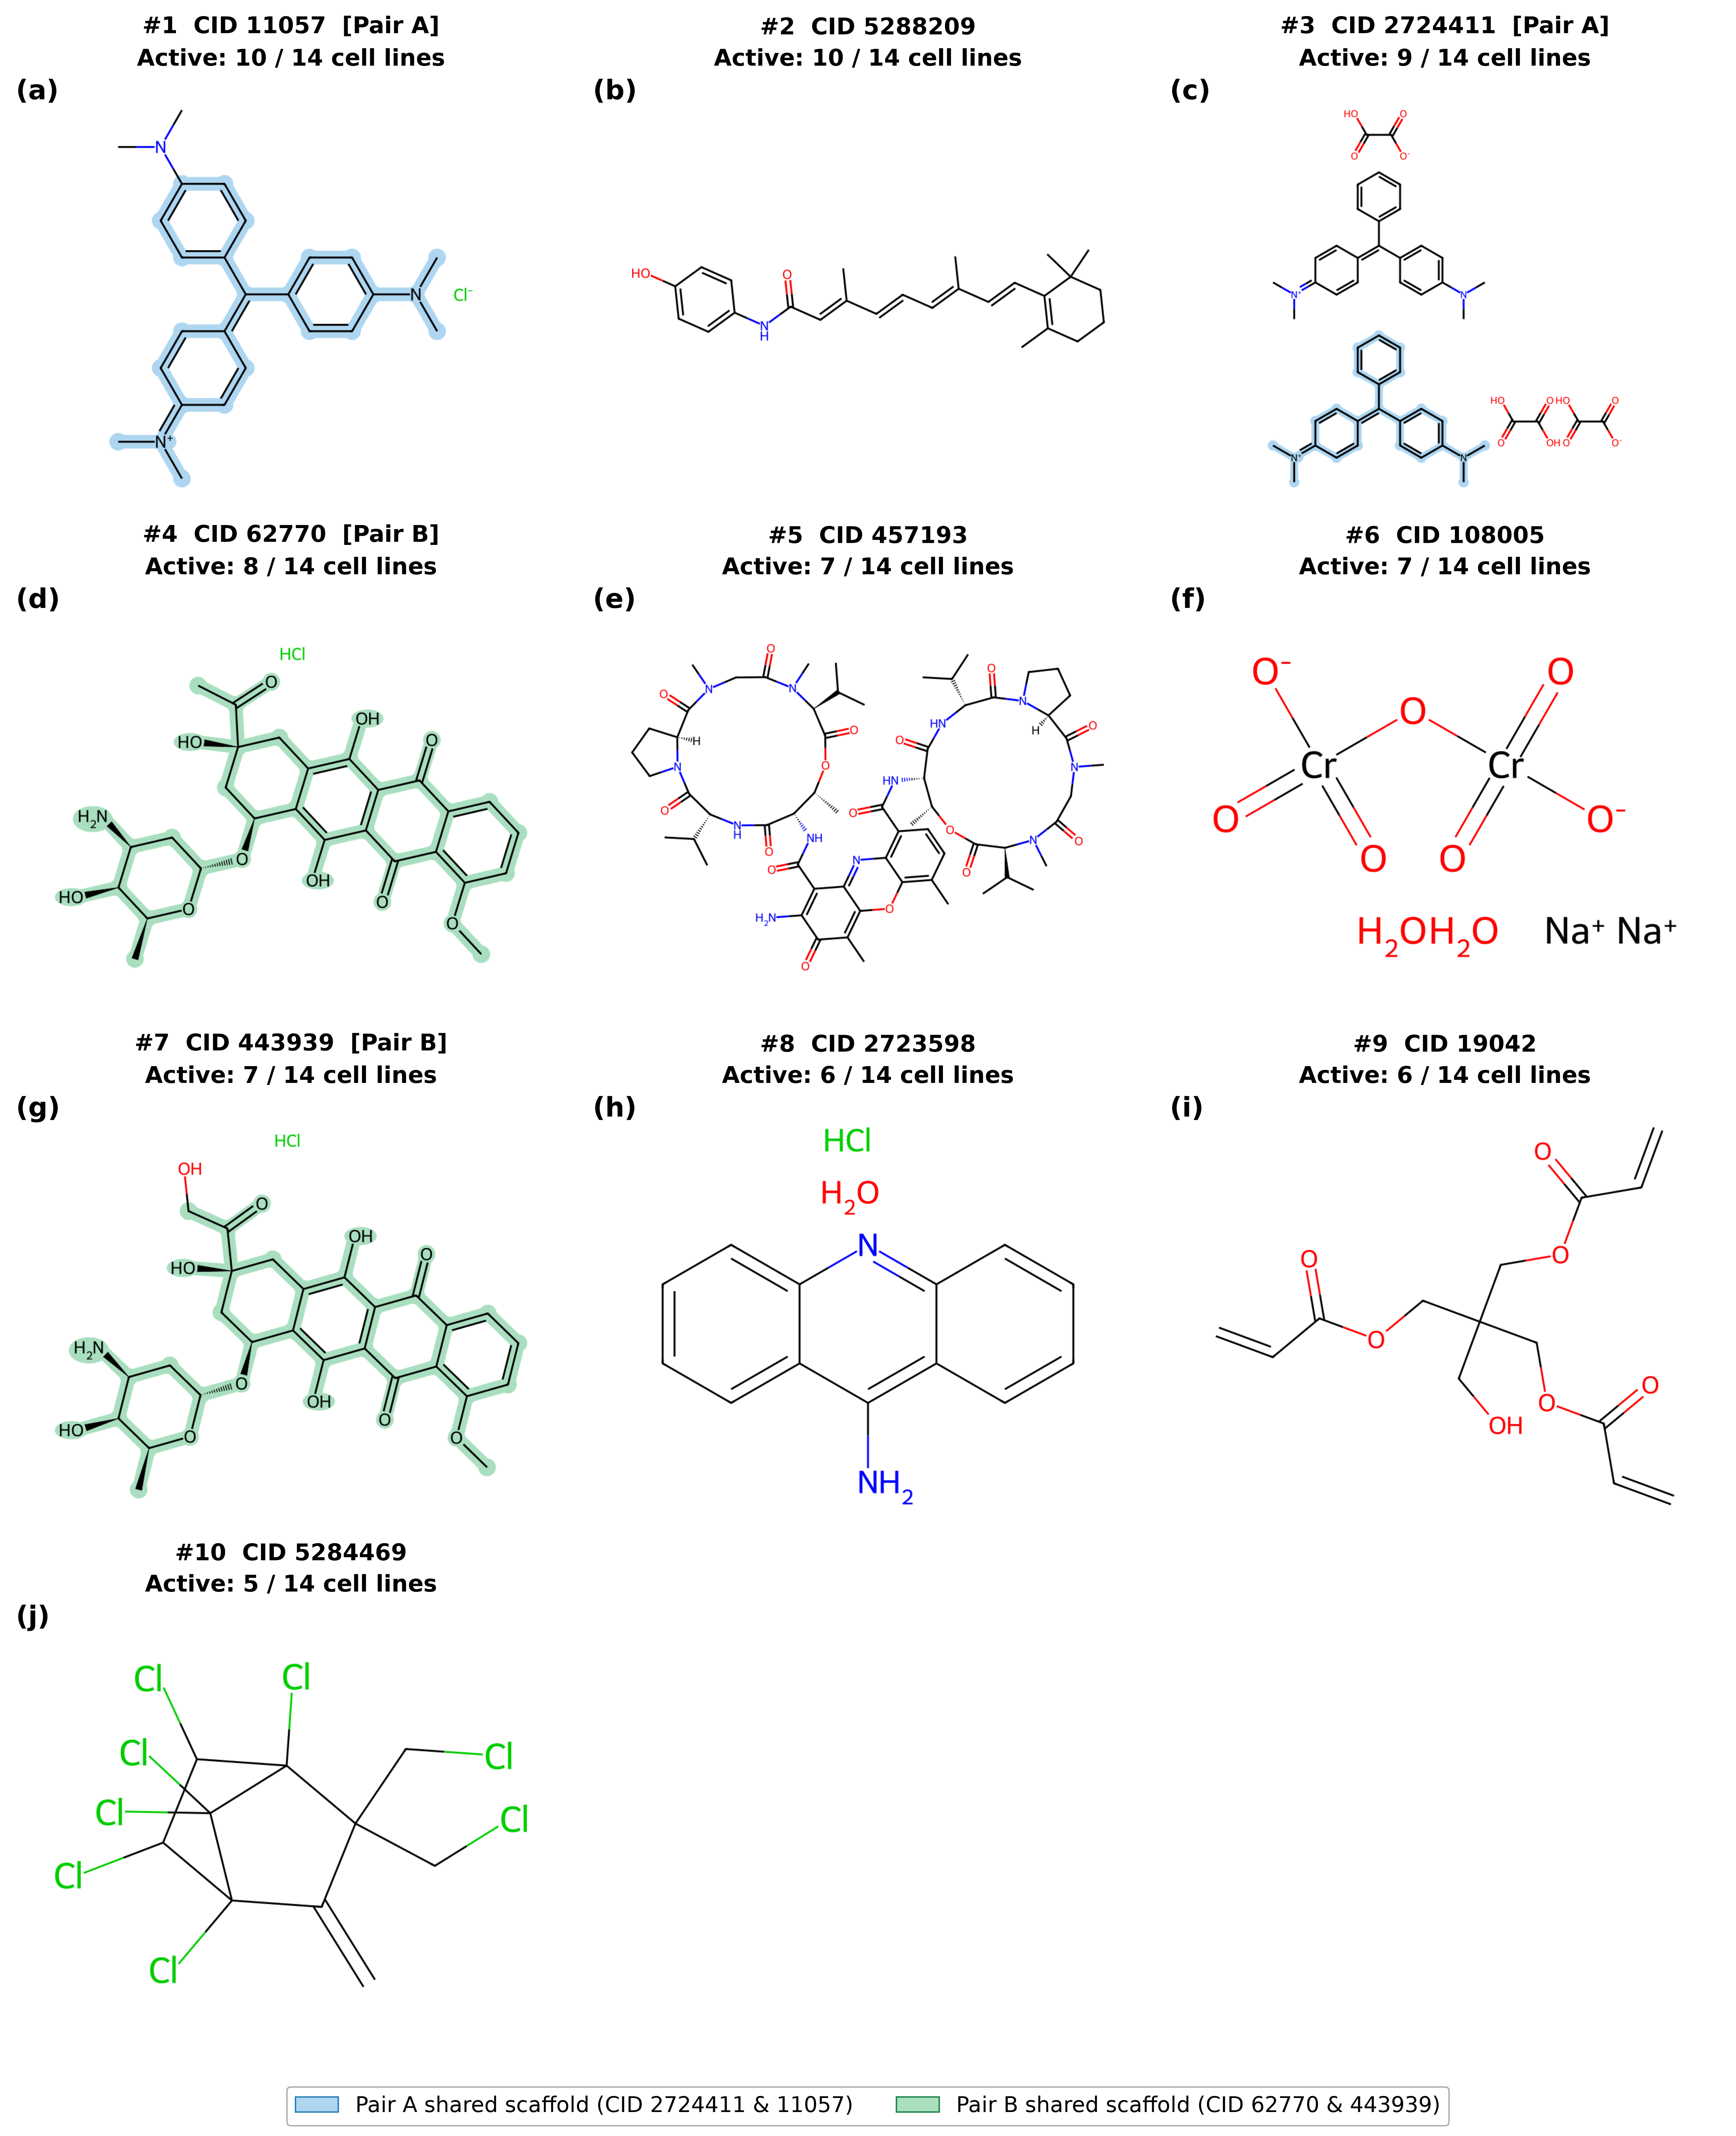
\includegraphics[width=0.9\linewidth]{figures/fig8_top10_structures_summary.png}
    \caption{Structures of the top ten most broadly active Caspase-3/7-activating compounds, sorted by decreasing number of active cell lines. The maximum common substructures (MCS) for two pairs of compounds are identified and highlighted: Pair A (CID 2724411 and 11057, blue) and Pair B (CID 62770 and 443939, green). The remaining six compounds share no significant common substructures.}
    \label{fig:top10_structures}
\end{figure*}

\begin{figure}[t!]
    \centering
    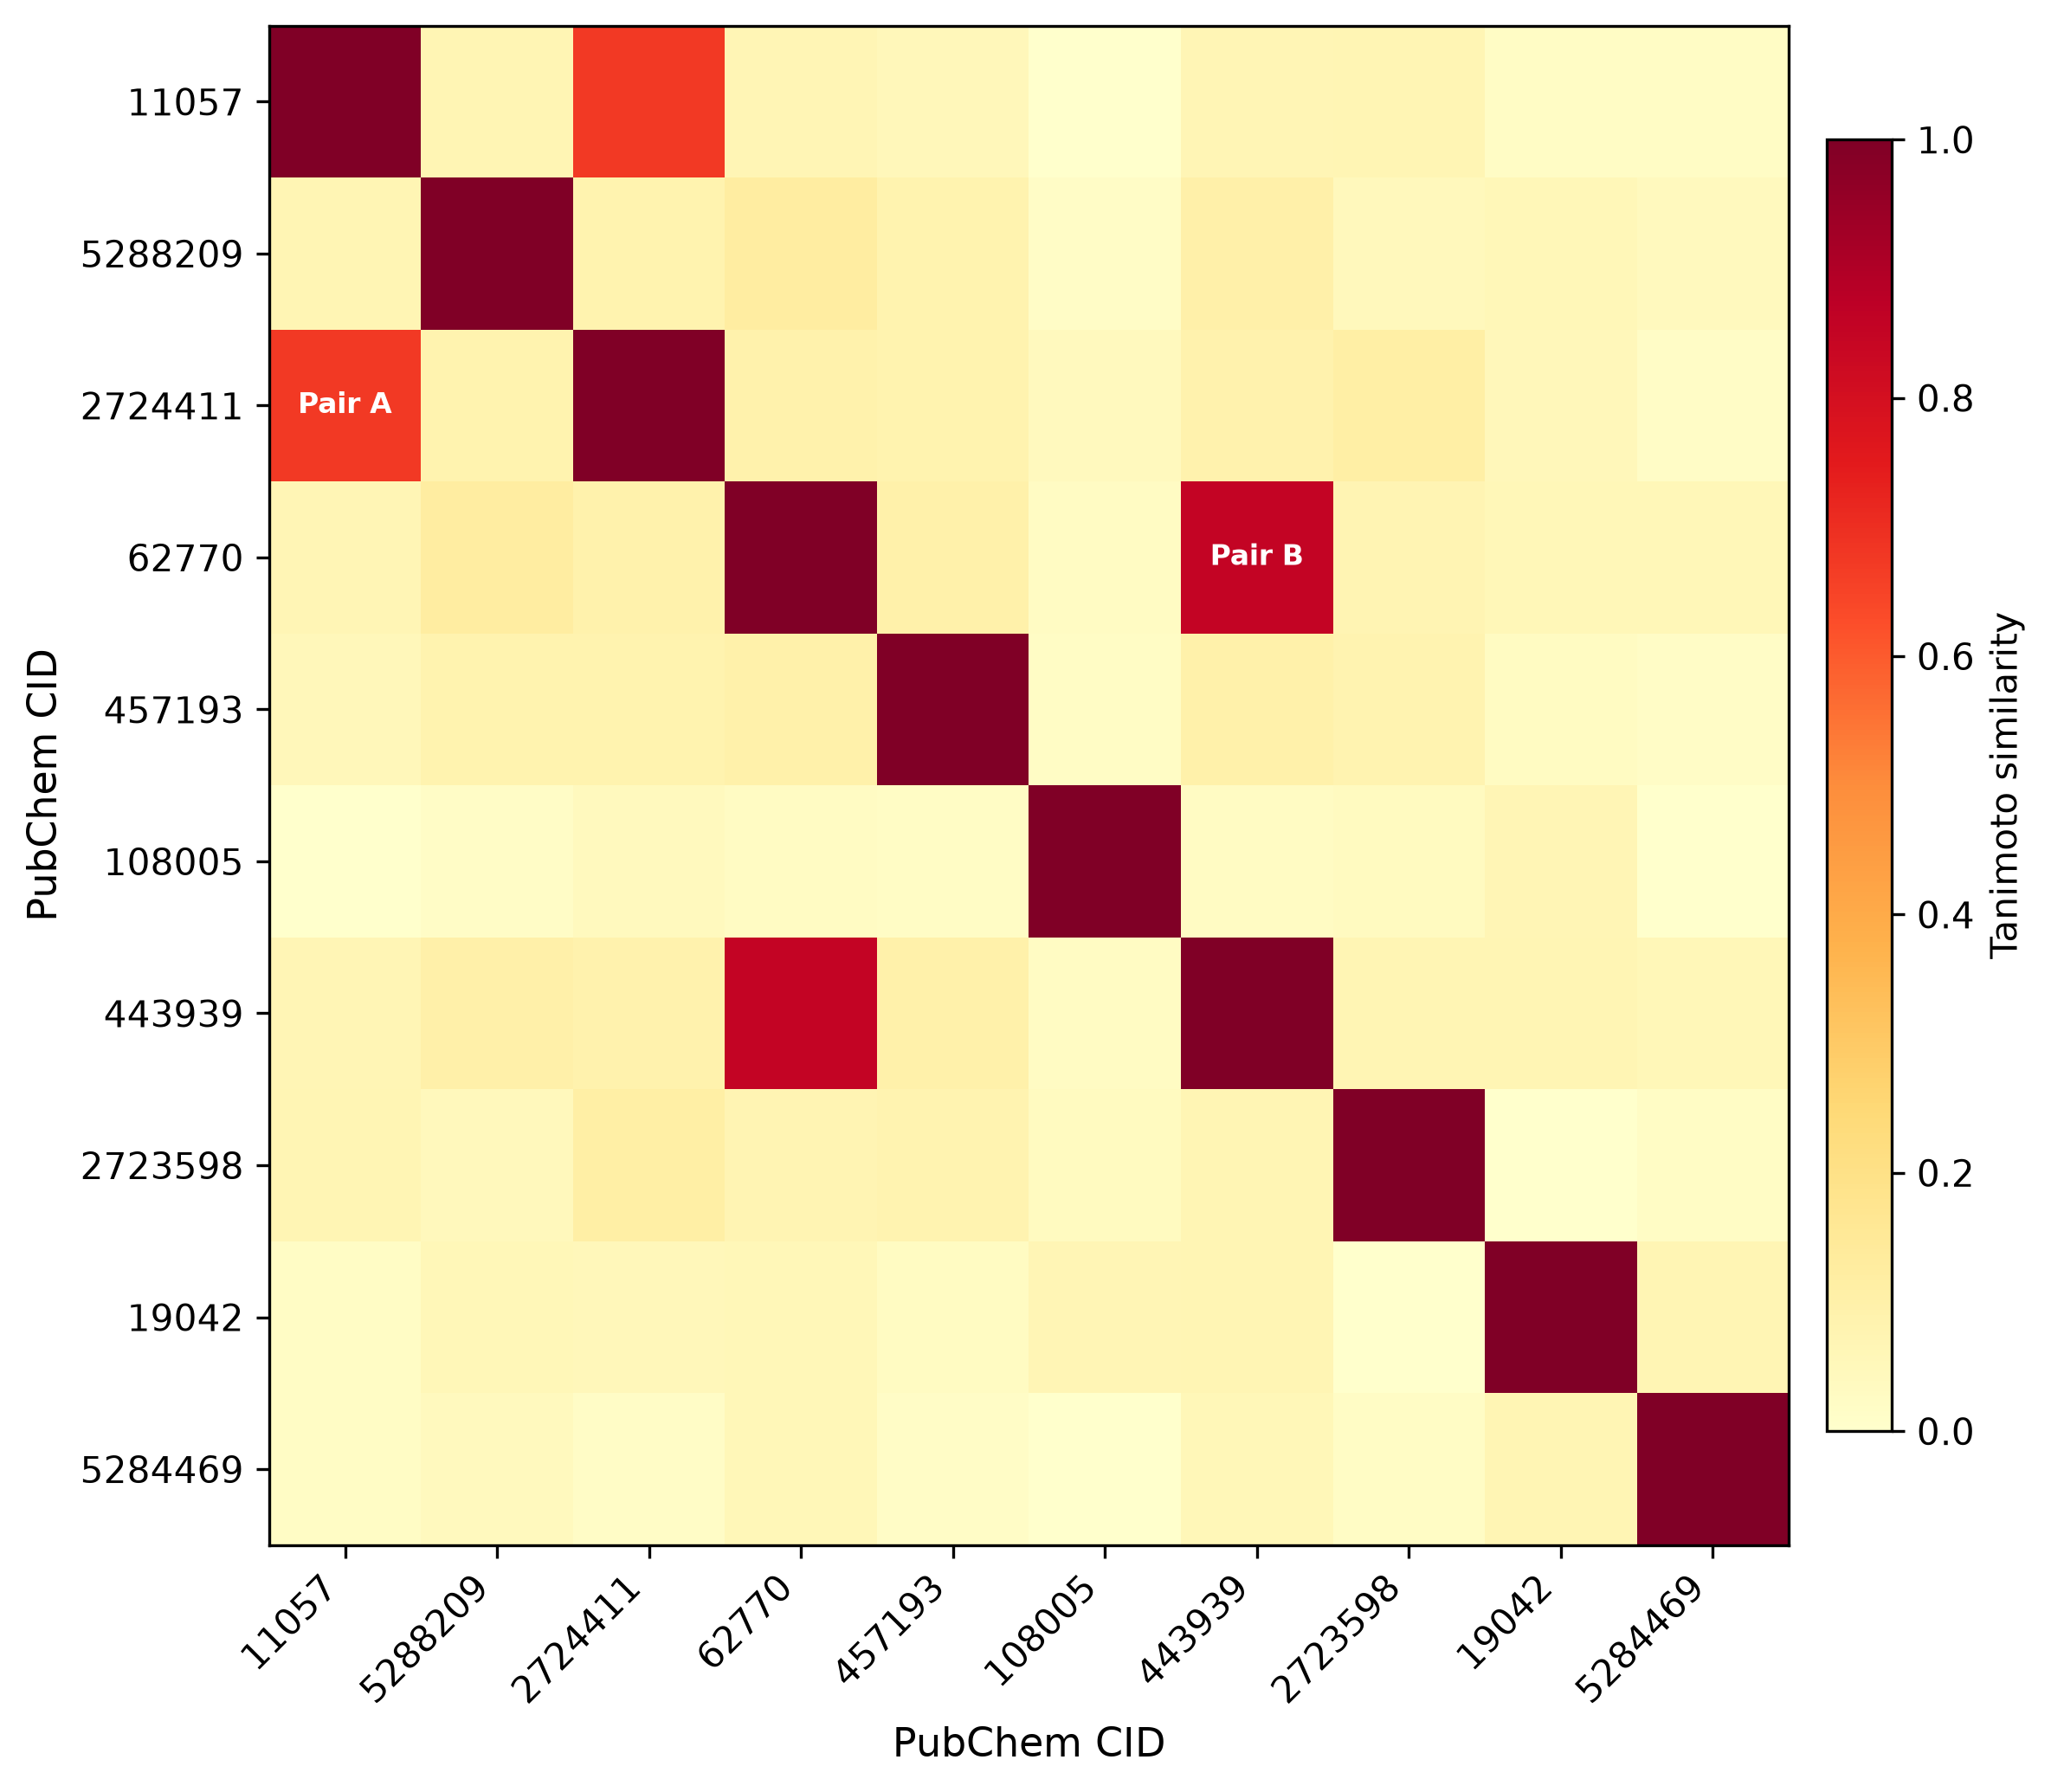
\includegraphics[width=0.5\linewidth]{figures/fig9_tanimoto_summary.png}
    \caption{Pairwise Tanimoto similarity between the ten most broadly active Caspase-3/7-activating compounds. Pairwise Tanimoto similarity matrix confirms low overall structural similarity across the set}
    \label{fig:top10_tanimoto}
\end{figure}


% --- HepG2 activation pattern vs clinical DILI status ---------------------
% ---------------------------------------------------------------------------
%  HepG2 activation pattern vs clinical DILI status  -- CONDENSED
%
%  Every number below was recomputed from DILI_assay_link/make_fig_dili_rate_panels.py.
%  Gold set = Held-223 + NCV-888 deduped (n = 1,098); 1,096 carry model
%  probabilities. Measured in both HepG2 summary assays: 197. Measured in the
%  MMP assay: 230. Measured in the Caspase-3/7 assay: 307.
%
%  The non-significance claim rests on Fisher's exact tests that the text no
%  longer spells out. For the record: per-assay subsets give OR = 1.71
%  (p = 0.37, n = 230) for MMP and OR = 1.04 (p = 1.0, n = 307) for
%  Caspase-3/7; restricted to the 197 measured in both, OR = 1.96 (p = 0.310)
%  and OR = 0.24 (p = 0.254). None is significant, so the claim holds on
%  either subset.
% ---------------------------------------------------------------------------

% --- Reviewer point: the consensus assay models are plugged into the DILI
% effort here, as grouping factors. Numbers recomputed from
% DILI_assay_link/make_fig_dili_rate_panels.py, which also prints the detail
% trimmed from the text below:
%   panel (B) label sources: 197 compounds with two measured calls,
%     143 with one measured and one predicted, 756 with two predicted
%   leak-free agreement under a 5-fold CV cutoff: MMP 90.9% +/- 2.5%,
%     Caspase-3/7 81.1% +/- 6.4% (the in-sample cutoff gives 95.2% / 85.0%,
%     which is optimistic because that cutoff is fitted on the same compounds)
%   non-significance: Fisher's exact, OR = 1.71 (p = 0.37, n = 230) for MMP and
%     OR = 1.04 (p = 1.0, n = 307) for Caspase-3/7
\paragraph{Relationship to Clinical DILI Status.}

To relate the assay models to the clinical endpoint, the consensus MMP and Caspase-3/7
models were used as grouping factors on the gold-standard DILI reference set:
Held-223 and NCV-888 combined and deduplicated by InChIKey, giving 1{,}098 compounds,
of which 710 (64.7\%) were considered toxic under the DILIst and DILIrank
classifications.

Each compound carries an active or inactive call in the HepG2 MMP summary assay
(AID~720637) and in the HepG2 Caspase-3/7 summary assay (AID~1347034); inconclusive
outcomes were excluded. Crossing the two calls gives four groups: inactive in both,
active in Caspase-3/7 only, active in MMP only, and active in both. Groups were
assigned from the \emph{in vitro} calls alone, and for each group the fraction of
toxic compounds was computed. In panel~(A) of
Figure~\ref{fig:dili_invitro_pattern}, for example, 17 compounds were active in MMP
and inactive in Caspase-3/7, of which 14 were toxic, a fraction of 82\%.

Only 230 reference compounds overlap with the MMP assay and 307 with the Caspase-3/7
assay, and 197 with both, leaving one compound active in Caspase-3/7 only and two
active in both, so the measured calls alone cannot answer the question (panel~A).
Panels~(B) and~(C) add predicted calls from the consensus assay models, which were
trained on the assay data and not on the reference set, using out-of-bag
probabilities thresholded at each model's Youden-$J$ cutoff (MMP 0.549; Caspase-3/7
0.268). Panel~(B) predicts only where a measured call is missing; panel~(C) predicts
throughout. Against the measured calls the models reached a ROC-AUC of 0.959 for MMP
and 0.936 for Caspase-3/7.

In all three panels the fraction of toxic compounds in the MMP-only group (82--87\%)
exceeded that of the set as a whole (64.6--67.0\%), while the Caspase-3/7-only group
was close to it. The ordering is not significant within the measured data, and the
dual-active group was not more enriched than the MMP-only group, so it is reported as
descriptive.

\begin{figure*}[t]
    \centering
    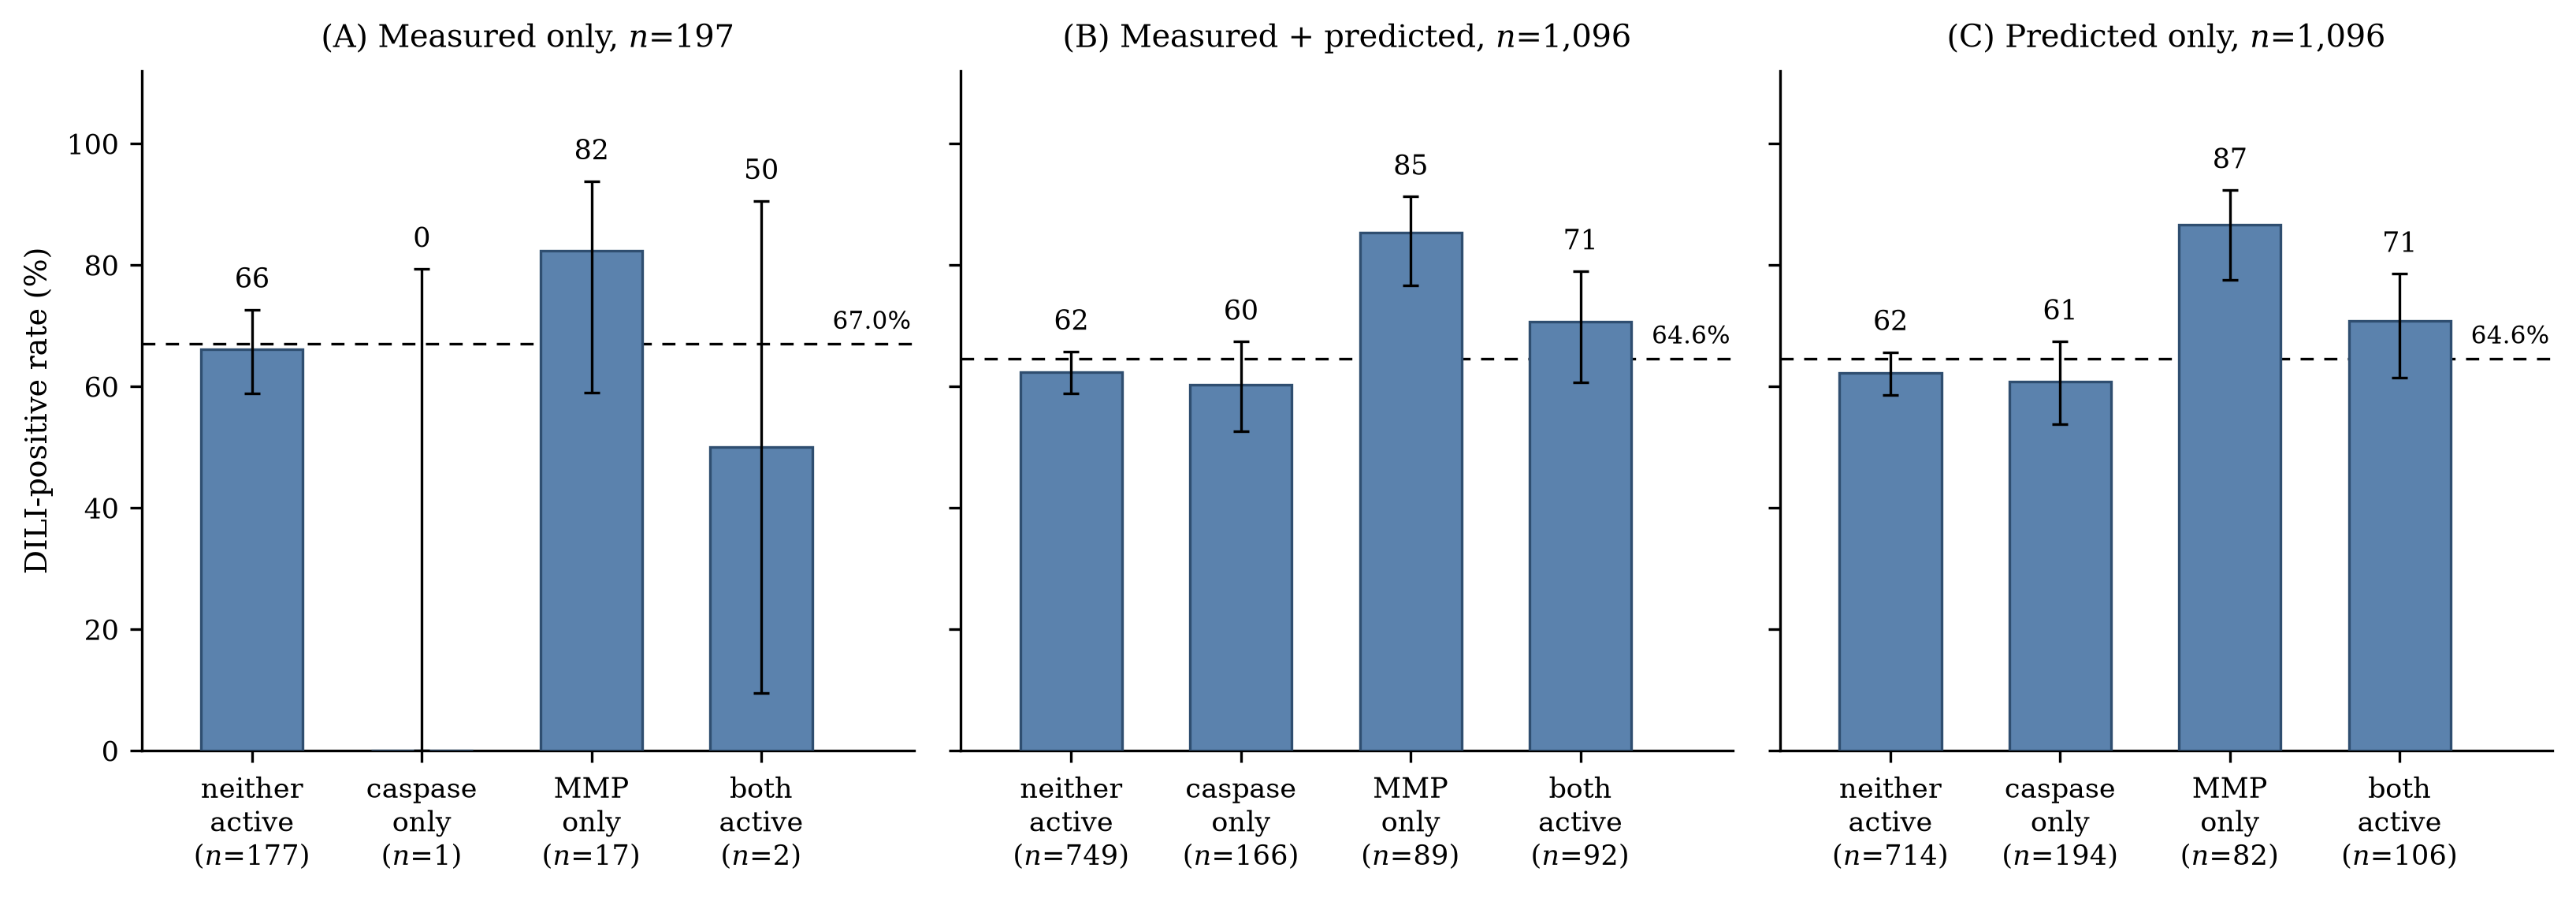
\includegraphics[width=\linewidth]{figures/fig_dili_rate_by_invitro_pattern.png}
    \caption{%
    Proportion of DILI-positive compounds among the gold-standard set, grouped by
    HepG2 \emph{in vitro} activation pattern (Caspase-3/7 $\times$ MMP).
    \textbf{(A)} Compounds measured in both HepG2 summary assays.
    \textbf{(B)} Measured labels where available, consensus-model predictions
    otherwise.
    \textbf{(C)} Consensus-model predictions throughout.
    Predicted labels use each consensus assay model's Youden-$J$ cutoff
    (MMP 0.549, Caspase-3/7 0.268); predictions are out-of-bag, so a compound's own
    measured label never enters its own prediction. The dashed line marks the
    DILI-positive base rate within each panel and category sizes are given beneath
    each bar. Error bars are 95\% Wilson intervals; in panels~(B) and~(C) these treat
    model-assigned labels as measurements and are therefore narrower than the true
    uncertainty. The caspase-only and dual-active categories in panel~(A) contain one
    and two compounds respectively, and their proportions are correspondingly
    uninformative.%
    }
    \label{fig:dili_invitro_pattern}
\end{figure*}


\subsubsection{Caspase Activations and Cell-Line-Specific Structural Motifs}

The only study on Caspase-3/7 activation prior to the present work is Huang et al. [12], who considered a “pan-Caspase-3/7 activator” by combining data from 13 different cell types and taking their average, and also identified structural features associated with pan-caspase toxicity. However, this approach does not account for the potential effects of cell-type heterogeneity on Caspase-3/7 activation, as different cell types may exhibit substantially different responses to the same compound or biological event. Consequently, their approach cannot provide a finer-grained cross-cell-line analysis or characterize differences in activation patterns among the tested cell lines. Similarly, their weighted feature significance method combines structural features across cell types for pan-caspase toxicity and therefore has the same limitation. For caspase toxicity prediction, their model performed slightly worse than the classical Naive Bayes model, whereas our results show that graph-based approaches, particularly graph transformers, and consensus models generally achieved stronger predictive performance. In the following, we provide a comprehensive analysis of cross-cell-line caspase activation and identify cell-line-specific structural motifs that are selectively associated with activation in individual cell types.



\paragraph{Chemical Structures of the Top Ten Most Broadly Active Compounds.}

We first analyze the structures resulting in the Caspase-3/7 activation for the largest number of cell lines. The top ten compounds, plotted in \textbf{Figure \ref{fig:top10_structures}}, impacted a significant number, five to ten out of the fourteen cell lines tested and their structural similarity were analyzed using pairwise Tanimoto similarity shown in \ref{fig:top10_tanimoto}. 
The similarity matrix in Figure~\ref{fig:top10_structures} reveals consistently low pairwise similarity across the set, indicating highly diverse structures can result in similarly broad caspase toxicity across multiple cell lines. We further performed a clustering analysis and extracted the common structure in each cluster. The Maximum Common Substructure (MCS)-based scaffold extraction was adopted, which is a cheminformatics approach used to identify the largest shared structural core among a group of compounds. Only two pairs of compounds exhibit notable scaffold overlap: compounds 2724411 and 11057 share a 25-atom scaffold, and compounds 62770 and 443939 share a 38-atom scaffold, as highlighted in Figure~\ref{fig:top10_structures}. The remaining six compounds form singleton clusters with no significant shared substructures.

Despite this structural diversity, all compounds demonstrate activity across multiple cell lines, suggesting that Caspase-3/7 activation is not driven by a single conserved scaffold but instead may arise from diverse chemotypes associated with complex cytotoxic mechanisms.

% \begin{table*}[t]
% \centering
% \small
% \caption{Top ten most broadly active compounds ranked by number of caspase cell-line assays in which they were classified as Active.}
% \label{tab:top10}
% \begin{tabular}{cccc}
% \toprule
% \textbf{PubChem CID} & \textbf{Cell Lines Active} & \textbf{MCS Cluster} & \textbf{MCS Atoms} \\
% \midrule
% 11057   & 10 & Pair A    & 25 \\
% 5288209 & 10 & Singleton & --- \\
% 2724411 & 9  & Pair A    & 25 \\
% 62770   & 8  & Pair B    & 38 \\
% 457193  & 7  & Singleton & --- \\
% 108005  & 7  & Singleton & --- \\
% 443939  & 7  & Pair B    & 38 \\
% 2723598 & 6  & Singleton & --- \\
% 19042   & 6  & Singleton & --- \\
% 5284469 & 6  & Singleton & --- \\
% \bottomrule
% \end{tabular}
% \end{table*}



\begin{figure}[t]
\centering
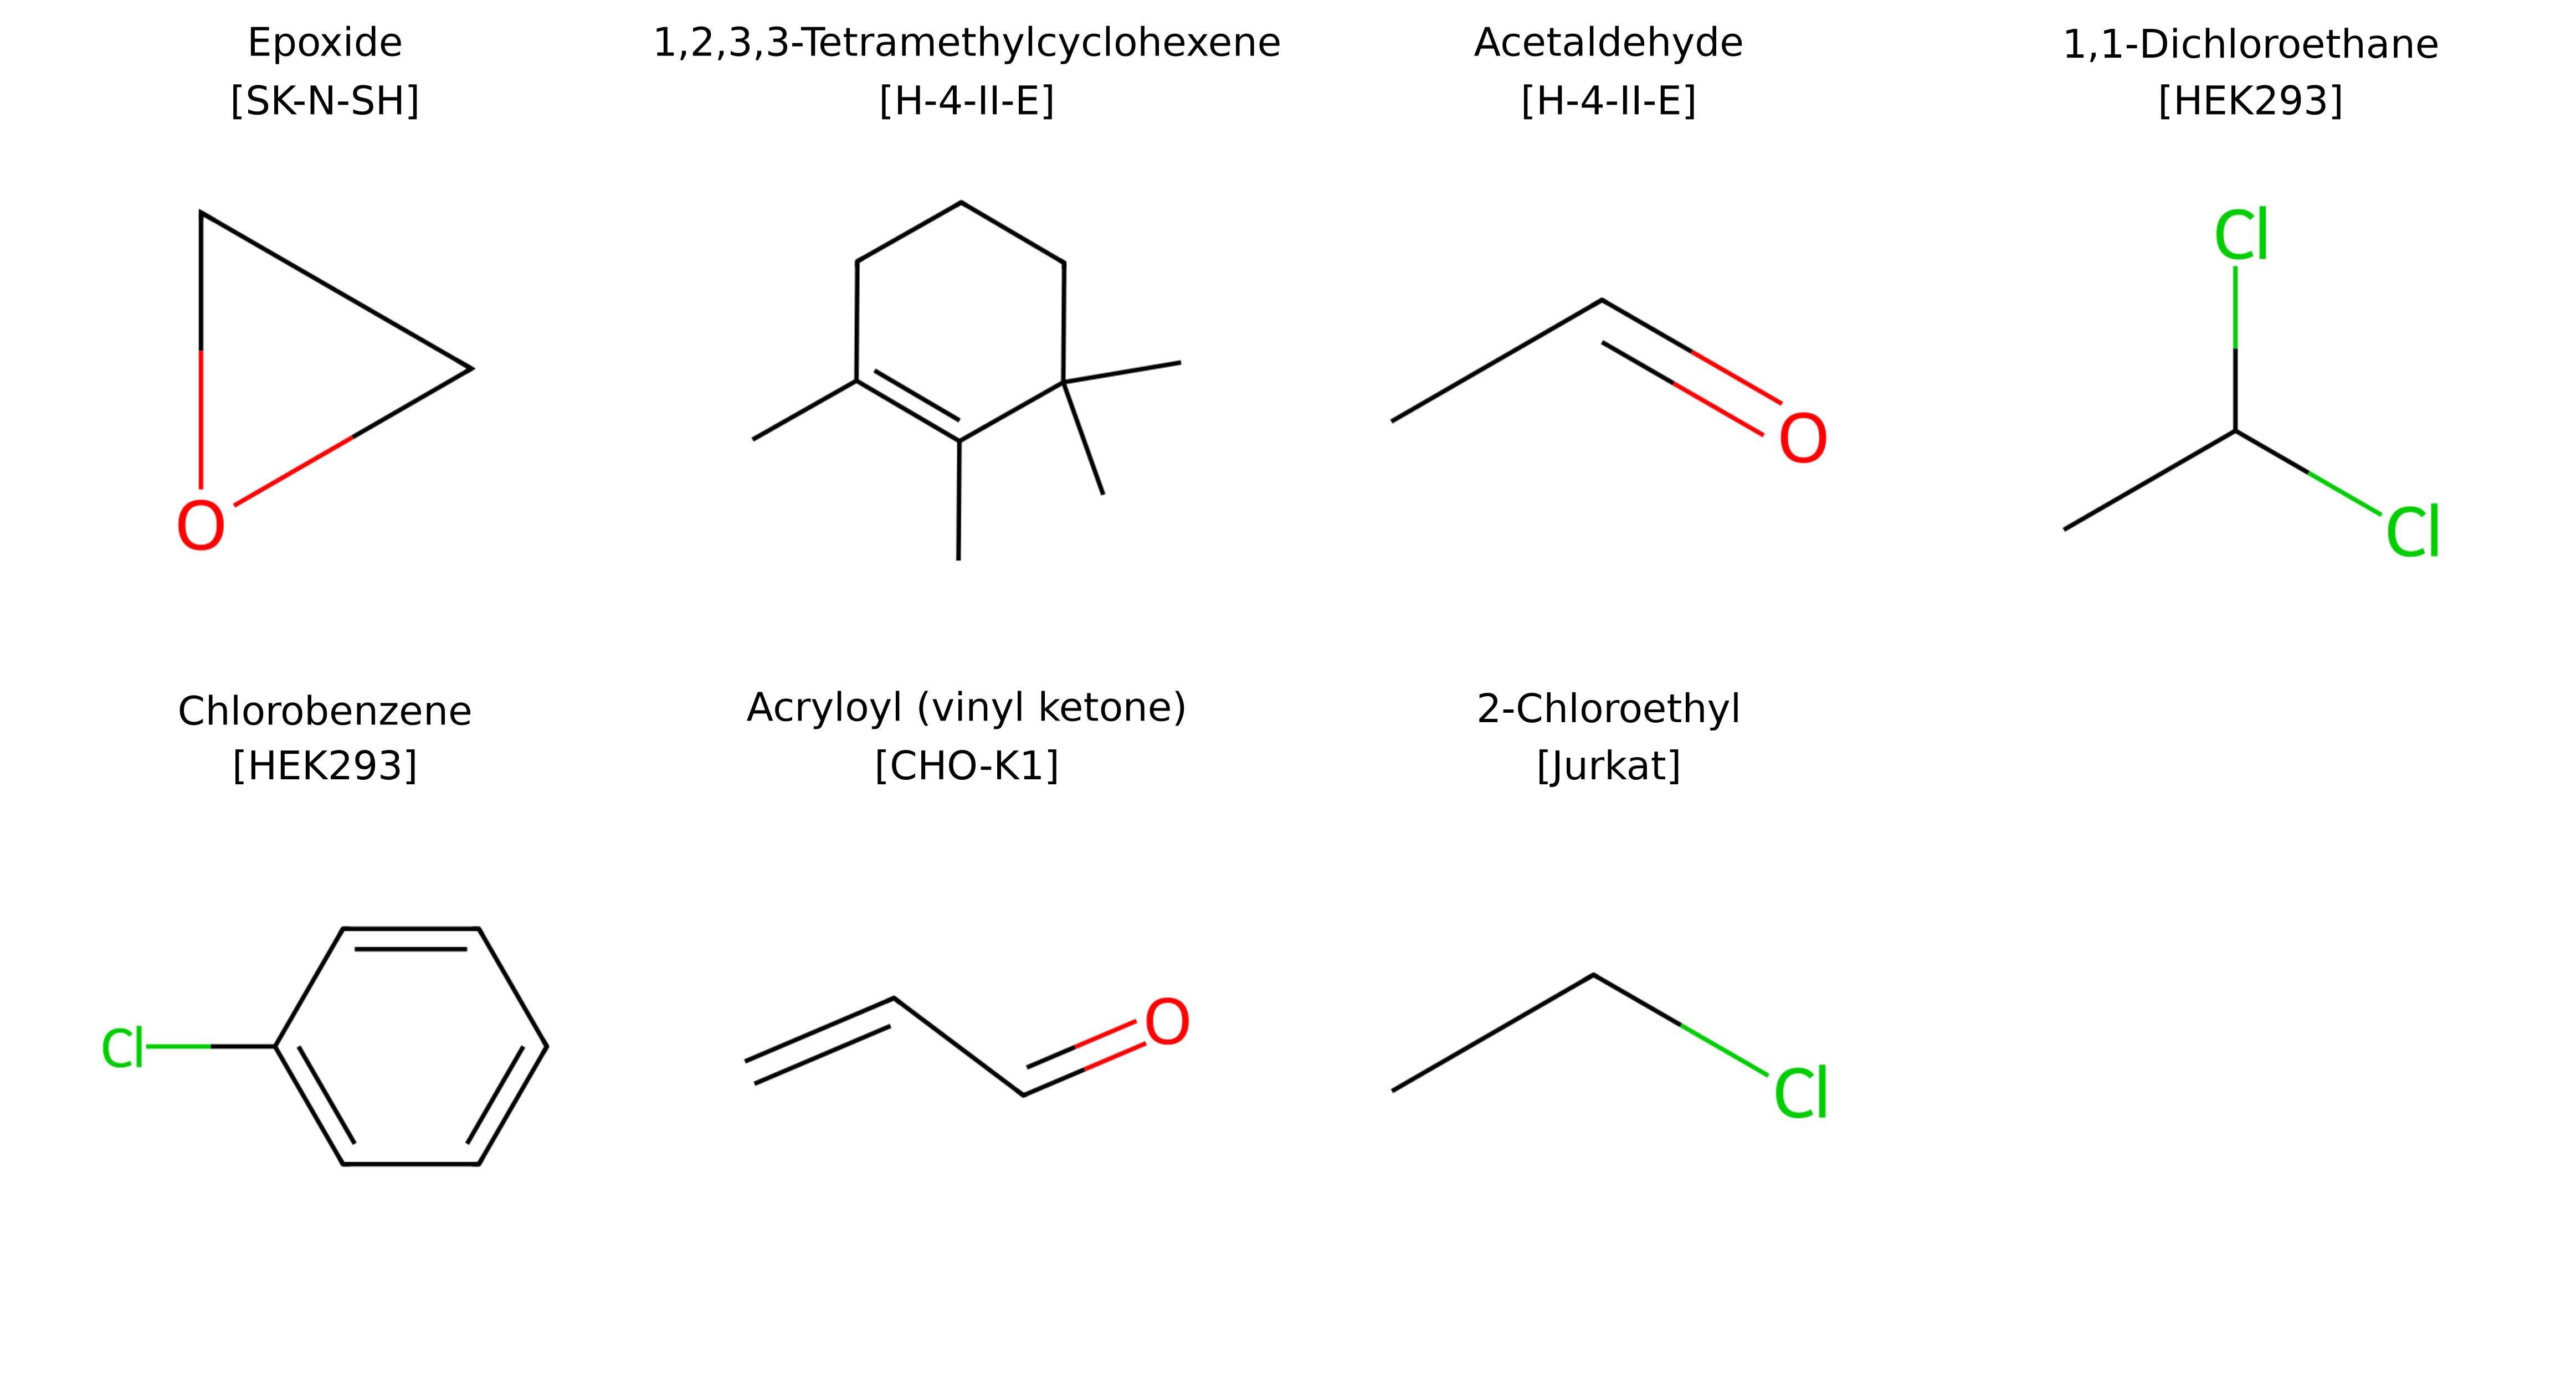
\includegraphics[width=0.8\linewidth]{figures/fig10_cellline_fragments_summary.png}
\caption{%
    BRICS fragments significantly enriched in \textbf{cell-line-specific} active
    compound sets. One fragment is unique to SK-N-SH; two are unique to
    H-4-II-E; two are unique to HEK293; one each is unique to CHO-K1 and
    Jurkat. No significant fragments were found for HepG2 or SH-SY5Y.
    Full enrichment statistics are in Supplementary Table S6.%\ref{tab:brics_cellline_enrichment}.
}
\label{fig:brics_cellline_fragments}
\end{figure}


\paragraph{Cell-Line-Specific Structural Motifs.}
To assess whether structural features predict cell-line selectivity, BRICS fragment enrichment was applied to each cell line. A one-sided Fisher's exact test compared fragments enriched in compounds active in a given cell line against compounds active in other cell lines. The FDR threshold was set to $\alpha = 0.10$ because several per-cell-line foreground groups were small ($n = 10$--$19$ active compounds); at $\alpha = 0.05$ the test is severely underpowered for groups of this size. Six cell lines with fewer than ten active compounds were excluded from further analysis. For the remaining eight cell lines, HepG2 ($n = 303$) and SH-SY5Y ($n = 10$) returned zero significant fragments, while CHO-K1 ($n = 171$), Jurkat ($n = 48$), SK-N-SH ($n = 19$), H-4-II-E ($n = 19$), HEK293 ($n = 17$) and NIH 3T3 ($n = 12$) produced enriched fragments. Seven fragments were enriched in exactly one cell line; these are illustrated in \textbf{Figure~\ref{fig:brics_cellline_fragments}}, with full enrichment statistics provided in Supplementary Table S8. The four fragments recovered for NIH 3T3 were each also enriched in at least one other cell line and are therefore not cell-line-specific. Five of the seven cell-line-unique fragments also satisfy the conventional $\alpha = 0.05$. Given the small per-cell-line sample sizes and the relaxed FDR threshold needed to retain statistical power at this scale, these enrichments are exploratory associations rather than confirmed determinants of cell-line selectivity, and would benefit from independent validation in larger or orthogonal datasets. With that caveat, HEK293 showed the most distinct structural pattern among those tested: 1,1-dichloroethane (OR~$= \infty$, $p_{\text{adj}} = 0.013$), absent from every other cell line, together with chlorobenzene (OR~$= 6.3$, $p_{\text{adj}} = 0.063$). SK-N-SH uniquely enriched an epoxide fragment (OR~$= 46.1$, $p_{\text{adj}} = 0.032$). H-4-II-E uniquely enriched a tetramethylcyclohexene motif (OR~$= 73.5$, $p_{\text{adj}} = 0.005$) and an acetaldehyde fragment (OR~$= 46.1$, $p_{\text{adj}} = 0.023$). CHO-K1 uniquely enriched an acryloyl group (OR~$= 16.5$, $p_{\text{adj}} = 0.031$) and Jurkat a 2-chloroethyl group (OR~$= 24.2$, $p_{\text{adj}} = 0.088$).

The observed differences in Caspase-3/7 activation across these cell lines can be attributed to the interplay between their chemical structures and the cell-specific capacity for biotransformation. In SK-N-SH neuroblastoma cells, the presence of an epoxide functional group introduces a highly reactive electrophilic center; this feature is capable of directly forming adducts with proteins and DNA, thereby triggering apoptotic signaling. Notably, neuroblastoma cells such as SK-N-SH lack certain detoxification enzymes (including microsomal glutathione S-transferase 1, or MGST1); this deficiency impairs the cells' ability to neutralize electrophilic intermediates, allowing these intermediates to persist and subsequently promote Caspase activation \cite{kelner2014absence}. Unlike in hepatic systems, CYP enzyme-mediated bioactivation is also relatively limited in SK-N-SH cells; this implies that in this specific cell line, direct chemical reactivity specifically the epoxide structure—rather than metabolic transformation, is the primary driver of apoptosis.
In contrast, the situation is markedly different in H-4-II-E cells, which are derived from hepatocytes; this distinction is primarily attributable to their robust capacity for xenobiotic metabolism. These cells express inducible CYP1A1/CYP1A2 and other Phase I metabolic enzymes, enabling them to convert lipophilic compounds—such as 1,2,3,3-tetramethylcyclohexene into reactive epoxide intermediates. Concurrently, aldehyde-containing structures (e.g., acetaldehyde) can undergo further transformation via metabolic pathways involving alcohol dehydrogenase (ADH) and CYP2E1, thereby generating electrophilic metabolites \cite{kaisarevic2015differential,markovic2022effect}. It is well established that within hepatocyte systems, these reactive species are capable of activating apoptotic signaling cascades and promoting the activation of Caspase-3/7 \cite{michels2006resveratrol}. Consequently, the robust metabolic capacity of H-4-II-E cells amplifies chemical toxicity by converting relatively inert lipophilic precursors into active electrophilic reagents; this also explains why these cells exhibit heightened sensitivity compared to non-hepatic cell lines.

Regarding HEK293 cells, it is well established that halogenated hydrocarbons disrupt cell membrane integrity and induce stress responses; these stress responses can subsequently trigger apoptosis via stress kinase pathways (e.g., JNK) and the downstream activation of Caspases \cite{michels2006resveratrol}. In contrast, SK-N-SH cells rely more heavily on direct electrophilic damage (e.g., from epoxides) to achieve robust Caspase activation; consequently, this cell line may exhibit a relatively attenuated response to the weaker stress signals generated by halogenated compounds. Furthermore, differences across cell types—specifically regarding their apoptotic priming status (e.g., the balance of Bcl-2 family proteins) and basal redox state—also influence the threshold required to trigger Caspase activation. 

% Our findings demonstrate that chemical structure alone is not the sole determinant of cytotoxicity; rather, the ultimate outcome of toxic effects depends on how different cell lines process these chemical structures. Specifically, in cells with limited metabolic capacity (such as SK-N-SH), electrophilic moieties (e.g., epoxides) directly drive Caspase activation; in metabolically active hepatic cell lines (such as H-4-II-E), toxicity is amplified through the generation of metabolic intermediates; whereas in systems with lower metabolic activity (such as HEK293), the cells’ heightened sensitivity to chemically induced stress (e.g., ER stress and oxidative stress) allows halogenated hydrocarbons—acting via membrane disruption and stress pathways like JNK—to directly trigger Caspase-3/7-mediated apoptosis without the need for potent electrophilic damage. This intrinsic link between chemical structure, biotransformation, and toxicological response provides a solid mechanistic basis for the cell-type-specific patterns of Caspase-3/7 activation that we have observed.





% \paragraph{Chemical Space Visualization.}

% We plotted the activation maps according to each cell line using UMAP projection. Figure \ref{fig:Hepg2_Active_Map_CL_main} shows the activation map for HepG2, the cell line with the highest number of active compounds, where the active compounds tend to locate in the left cluster of the chemical space. Activation maps for all the cell lines are provided in Appendix~\ref{sec:appendix_remaining_cells} (Figure~\ref{fig:Active_Map_CL_supp}). The dark colored points represent compounds that are consistently active for a large number of cell lines, e.g., 5--10 lines.


% \begin{figure*}[htbp]
%     \centering
%     \includegraphics[width=0.8\linewidth]{figures/Hepg2_Map_CL_celline.png}
%     \caption{Distribution of compounds in the chemical space for the HepG2 cell line.}
%     \label{fig:Hepg2_Active_Map_CL_main}
% \end{figure*}



% \subsubsection*{Apoptosis via Caspase-3/7 Activation}

% The total number of unique compounds after merging
% all the fourteen cross-cell-line \emph{Caspase-3/7} assays was 7,716. Out of these, 323 compounds (4.2\%) showed Caspase-3/7
% activation in at least one cell line. There are 1,272 compounds that were fully tested for all fourteen cell lines, i.e., they have Caspase-3/7 activity outcome for every cell line. Out of these, 104 compounds (8.2\%) showed Caspase-3/7 activation in at least one cell line. In addition, there are 66 compounds that were tested as Caspase-3/7 active in both non-human CHO-K1 and human HepG2 cell lines while not tested in the other twelve cell lines.


% \paragraph{Clustering Analysis of Caspase-Active Compounds.}

% To study whether there are well-defined groups in caspase-active compounds across cell lines, clustering analysis was performed on two complementary groups: \textit{fully-tested group}: 104 compounds tested across all 14 cell-line assays and active in at least one cell line, and \textit{cross-species group}: 66 compounds tested exclusively in CHO-K1 and HepG2 and active in both cell lines. We applied clustering analysis on these compounds to group similar compounds into the same cluster, followed by finding common substructures within each cluster. DBSCAN~\cite{ester1996dbscan} can identify clusters of any shape and automatically identifies noise points, which is suitable for the non-spherical, heterogeneous distributions of chemical space. Detailed settings of the clustering can be found in Appendix \ref{apx:clustering}.

% % Among the 104 fully-tested compounds, DBSCAN identified 12 structural
% % clusters (18 noise points), spanning distinct compound families
% % including aminophenols (C0; $n = 16$), anthracyclines such as
% % doxorubicin (C5; $n = 10$), triarylmethane dyes such as Malachite Green
% % (C3; $n = 15$), alkylphenols (C9; $n = 6$), organochlorines including
% % technical chlordane and p,p$'$-DDD (C10--C11), and heavy-metal
% % compounds such as sodium dichromate (C8). 

% % Pan-toxic compounds (active
% % in $\geq 8$ cell lines; $n = 4$) were distributed across multiple
% % clusters rather than concentrated in one structural family
% % (Figure~\ref{fig:umap_104_breadth}).

% For the combined 170-compound set, DBSCAN yielded 
% 13 clusters with only 10 noise points. Of the 13 clusters, 11 contained 
% compounds from both the fully-tested and cross-species groups, indicating 
% that the same structural families responsible for Caspase-3/7 activation 
% across 14 cell lines also drive cross-species (human/hamster) co-activation. 
% The five largest clusters are shown in Figure~\ref{fig:grid_170_main}: 
% phenylenediamines and anilines (C2; $n = 20$), antihistamine-like piperidine 
% scaffolds (C11; $n = 19$), anthracyclines (C7; $n = 18$), alkylphenols 
% (C5; $n = 17$), and dichlorophen-related chlorinated biphenyls (C4; $n = 16$). 
% Together these five clusters account for 90 of the 160 clustered compounds. 
% The remaining eight clusters, including retinoids (C0; $n = 13$), triarylmethane 
% dyes (C9; $n = 13$), and organochlorines (C10; $n = 4$), are detailed in 
% Appendix~\ref{sec:grid_170_full}.





% These results demonstrate that Caspase-3/7-activating structural motifs
% are not specific to any single testing context. The complete structural
% overlap between the two groups suggests that cross-species caspase
% induction is driven by the same mechanistic chemotypes regardless of
% whether compounds were characterised in the full 14-cell-line panel or
% only in the two-cell-line CHO-K1/HepG2 screen.

% Common substructure analyses were also performed on the 323 compounds that are active in at least one cell line as well as the entire set of 7,716 compounds. The observations on the 323 active compounds are similar to the 170 compounds
% discussed above. The full details are deferred to Appendix~\ref{sec:appendix_323}. The whole set of compounds exhibits 42 clusters, with 4,198 compounds in a
% dominant cluster whose shared common substructure is Ethyl Benzoate and 1,863 compounds in another large cluster whose shared substructure is Ethyl Heptanoate.


% \begin{figure*}[htbp]
%     \centering
%     \includegraphics[width=\linewidth]{umap_104_activity_breadth}
%     \caption{UMAP projection of ECFP4 fingerprints for the 104
%     fully-tested caspase-active compounds, coloured by activity breadth.
%     Pan-toxic compounds (active in $\geq 8$ cell lines; $n = 4$, red)
%     are distributed across chemical space rather than forming a single
%     structural cluster.}
%     \label{fig:umap_104_breadth}
% \end{figure*}

% \begin{figure*}[t]
%     \centering
%     \includegraphics[width=\linewidth]{umap_170_mixed_clusters}
%     \caption{UMAP projection of the combined 170 caspase-active
%     compounds (104 fully-tested, circles; 66 CHO-K1+HepG2, triangles),
%     coloured by structural cluster. All 13 DBSCAN clusters contain
%     compounds from both groups, demonstrating that the same scaffold
%     families underlie Caspase-3/7 activation regardless of assay
%     coverage.}
%     \label{fig:umap_170_mixed}
% \end{figure*}

% \begin{figure*}[t]
%     \centering
%     \includegraphics[width=0.8\textwidth]{figures/170_compounds_main_grid.png}
%     \caption{Representative structures and MCS cores for the five largest
%     structural clusters identified among the 170 combined caspase-active
%     compounds. For
%     each cluster, the MCS core (shared scaffold, highlighted in red) is
%     shown alongside up to five central representative molecules. The five
%     clusters account for 90 of the 160 clustered compounds:
%     phenylenediamines and anilines (C2; $n = 20$), antihistamine-like
%     piperidines (C11; $n = 19$), anthracyclines (C7; $n = 18$),
%     alkylphenols (C5; $n = 17$), and chlorinated biphenyls (C4;
%     $n = 16$).}
%     \label{fig:grid_170_main}
% \end{figure*}






% \paragraph{Caspase and Mitochondrial Co-Active Compounds: Fragment
% Enrichment Analysis.}

% The caspase--mitochondrial comparison (HepG2) yielded three mutually
% exclusive active groups: 288 compounds co-active in both assays
% (\textit{Both Active}), 34 compounds active in the caspase assay only
% (\textit{Caspase Only}), and 1,944 compounds active in the mitochondrial
% assay only (\textit{Mito Only}), for a total of 2,266 active compounds
% (Table~\ref{tab:active_groups}).

% \begin{table}[t]
% \centering
% \small
% \caption{Active compound groups used in caspase--mitochondrial
% substructure analysis.}
% \label{tab:active_groups}
% \begin{tabular}{lc}
% \hline
% \textbf{Activity Group} & \textbf{Compounds} \\
% \hline
% Both Active (caspase $+$ mito) & 288     \\
% Caspase Only                   & 34      \\
% Mito Only                      & 1{,}944 \\
% \hline
% \textbf{Total Active} & \textbf{2{,}266} \\
% \hline
% \end{tabular}
% \end{table}


% \begin{table*}[t]
% \centering
% \small
% \caption{Top enriched BRICS fragments in dual-active (caspase $+$ mito)
% vs.\ single-active compounds, ranked by $p$-value. OR = odds ratio;
% $n_{\text{both}}$ = count in dual-active set;
% $n_{\text{single}}$ = count in single-active set.}
% \label{tab:fisher_enrichment}
% \begin{tabular}{p{3.8cm}ccccc}
% \hline
% \textbf{Fragment} & \textbf{Structure} & \textbf{OR} &
% \textbf{\textit{p}-value} & $n_{\text{both}}$ & $n_{\text{single}}$ \\
% \hline

% Aminosugar moiety &
% \includegraphics[width=1.6cm,height=1.6cm,keepaspectratio]{fragment_table14_a.png} &
% $\infty$ & $6.25\times10^{-8}$ & 8 & 0 \\[6pt]

% Anthracycline ring system &
% \includegraphics[width=1.6cm,height=1.6cm,keepaspectratio]{fragment_table14_b.png} &
% $\infty$ & $6.25\times10^{-8}$ & 8 & 0 \\[6pt]

% Methylphenol motif &
% \includegraphics[width=1.6cm,height=1.6cm,keepaspectratio]{fragment_table14_c.png} &
% $\infty$ & $4.03\times10^{-6}$ & 6 & 0 \\[6pt]

% Trialkyltin fragment &
% \includegraphics[width=1.6cm,height=1.6cm,keepaspectratio]{fragment_table14_d.png} &
% $\infty$ & $4.03\times10^{-6}$ & 6 & 0 \\[6pt]

% Long-chain alkyl (C12) &
% \includegraphics[width=1.6cm,height=1.6cm,keepaspectratio]{fragment_table14_e.png} &
% 21.0 & $8.99\times10^{-5}$ & 6 & 2 \\[6pt]

% Quaternary ammonium &
% \includegraphics[width=1.6cm,height=1.6cm,keepaspectratio]{fragment_table14_f.png} &
% 21.0 & $8.99\times10^{-5}$ & 6 & 2 \\[6pt]

% Branched C8 alkyl (isooctyl-type) &
% \includegraphics[width=1.6cm,height=1.6cm,keepaspectratio]{fragment_table14_g.png} &
% 21.0 & $8.99\times10^{-5}$ & 6 & 2 \\[6pt]

% Long-chain alkyl (C12, alt.) &
% \includegraphics[width=1.6cm,height=1.6cm,keepaspectratio]{fragment_table14_h.png} &
% 21.0 & $8.99\times10^{-5}$ & 6 & 2 \\[6pt]

% Hydroxyphenylene bridge &
% \includegraphics[width=1.6cm,height=1.6cm,keepaspectratio]{fragment_table14_i.png} &
% 5.89 & $1.50\times10^{-4}$ & 10 & 12 \\[6pt]

% \hline
% \end{tabular}
% \end{table*}

% We use the Breaking Retrosynthetically Interesting Chemical Substructures (BRICS) method \cite{degen2008art} (as implemented
% in RDKit) to decompose the 288 dual-active compounds into 862 fragment occurrences across 235 unique fragments. A
% one-sided Fisher's exact test identified 147 fragments significantly
% enriched in the dual-active set relative to the 1,978 single-active
% compounds ($p < 0.05$, OR $> 1$).
% As shown in Table~\ref{tab:fisher_enrichment}, four fragments were found exclusively in dual-active compounds: an aminosugar moiety and an
% anthracycline-derived ring system, and a methylphenol motif together with a trialkyltin fragment. Four additional fragments
% were strongly enriched:
% two long-chain alkyl chains, a quaternary ammonium group, and a
% di-\textit{tert}-butylmethyl fragment. A para-hydroxyphenyl motif showed moderate enrichment. Together, these motifs encompass
% membrane-intercalating hydrophobic chains, organotin compounds with
% established mitochondrial toxicity, and redox-active phenolic
% scaffolds - structural classes consistent with mitochondrial membrane
% disruption and caspase-mediated apoptosis.

%Removing the section mitochondrial pathway and cytotoxicity
% \subsubsection{Mitochondria Pathway and Cytotoxicity}
% Remove this sub
% Since the cytotoxicity in terms of the cell viability in the same assay well of MMP assay is also available, we conducted pairwise comparison of MMP activity and cell viability in \textbf{Table~\ref{tab:mito_viability}}. As shown in Table~\ref{tab:mito_viability}, 6\% of compounds were active in both MMP activity and cell viability. Notably, no compounds were found that were mitochondria-inactive and viability-active, indicating that the cell viability loss does not occur independently of MMP disruption under these assay conditions.

% \begin{table}[t]
% \centering
% \small
% \caption{Pairwise comparison of mitochondrial activity and
% cell viability in HepG2 cells.}
% \label{tab:mito_viability}
% \begin{tabular}{lc}
% \hline
% \textbf{Category} & \textbf{Count} \\
% \hline
% Both active                             & 292 (6\%)    \\
% Mitochondria active, viability inactive & 680 (16.3\%)     \\
% Mitochondria inactive, viability active & 0       \\
% Both inactive                           & 3{,}196  (76.7\%)\\
% \hline
% % \textbf{Total} & \textbf{4{,}168} \\
% % \hline
% \end{tabular}
% \end{table}

% \begin{figure*}[t!]
% \centering
% \includegraphics[width=0.82\linewidth]{figures/fig_mito_viab_t7_fragments.png}
% \caption{%
%     BRICS fragments significantly enriched in compounds active in both the
%     mitochondrial membrane potential and cell viability assays versus compounds
%     inactive in both (HepG2; $n_{\text{active}} = 292$,
%     $n_{\text{inactive}} = 3{,}196$; FDR $\alpha = 0.01$). Fragments are
%     grouped by structural family; all 17 significant motifs are shown. Full
%     enrichment statistics (OR, 95\,\% CI, $p_{\text{adj}}$, prevalence) are
%     provided in Supplementary Table S4.%\ref{tab:brics_t7_enrichment}.
% }
% \label{fig:brics_t7_fragments}
% \end{figure*}


% \paragraph{Structural Motifs Associated with Dual Mitochondrial and Cell Viability 
% Activity.}
% To identify structural features associated with simultaneous mitochondrial 
% membrane disruption and reduced cell viability, BRICS fragment enrichment was 
% applied to compounds active in both assays ($n = 292$) against compounds 
% inactive in both ($n = 3{,}196$; one-sided Fisher's exact test, 
% Benjamini--Hochberg FDR $\alpha = 0.01$). Seventeen fragments reached 
% significance across eight structural families; these are illustrated in 
% \textbf{Figure~\ref{fig:brics_t7_fragments}}, with full enrichment statistics provided 
% in Supplementary Table S4.%\ref{tab:brics_t7_enrichment}.

% The phenolic family produced four enriched motifs. Para-hydroxyphenyl 
% (phenol) was the top-ranked fragment overall based on $p_{\text{adj}}$ ($p_{\text{adj}} = 6.0 \times 10^{-6}$), followed by 4-chlorophenol 
% ($p_{\text{adj}} = 4.7 \times 10^{-4}$), pyrogallol 
% ($p_{\text{adj}} = 2.9 \times 10^{-3}$), and \textit{m}-cresol 
% ($p_{\text{adj}} = 2.9 \times 10^{-3}$), all of which are absent from the 
% dual-inactive set. Dimethylamine was the only nitrogen-containing fragment and 
% carried the highest point estimate among rank-2 families 
% ($p_{\text{adj}} = 1.7 \times 10^{-5}$). Trifluoromethyl was the 
% sole halogenated motif and ranked third overall ($p_{\text{adj}} = 2.7 \times 10^{-5}$). Among organophosphates, 
% O,O-dimethyl thiophosphate
% and phosphate triester 
% produced the largest point estimates in the analysis, consistent with known 
% organophosphate cytotoxicity mechanisms. Tributyltin alkoxide, the sole 
% organometallic fragment, was absent from the dual-inactive set, reflecting the 
% well-established mitochondrial toxicity of organotin compounds. The lipophilic 
% chain family contributed four fragments---\textit{tert}-butyl, 2,2,4-trimethylpentyl, methine carbon, and octyl chain---indicating that 
% branched and linear lipophilic extensions are a recurrent structural feature 
% of dual-toxic compounds, likely facilitating membrane partitioning. 
% Nitroaromatic and chlorinated aromatic fragments each yielded two enriched 
% motifs at lower significance (both families $p_{\text{adj}} \leq 
% 7.6 \times 10^{-3}$).



% % \paragraph{Structural Comparison of Dual-Toxic versus Mitochondria-Only
% % Active Compounds.}
% % To determine whether compounds that combine MMP disruption with cell
% % viability loss ($n = 292$) are structurally distinct from those that
% % disrupt MMP alone ($n = 680$), BRICS fragment enrichment was applied
% % between the two groups (one-sided Fisher's exact test,
% % Benjamini--Hochberg FDR $\alpha = 0.10$, $\text{min\_count} = 2$).
% % No fragment reached significance, indicating that the two groups share
% % essentially the same chemical scaffolds.

% \paragraph{Structural Motifs Associated with Mitochondria-Only
% Active Compounds.}

% \begin{figure*}[t!]
% \centering
% \includegraphics[width=\linewidth]{figures/fig_mito_mito_only_vs_both_inactive.png}
% \caption{%
%     Top twelve BRICS fragments enriched in mitochondria-active,
%     viability-inactive compounds versus dual-inactive compounds
%     (HepG2; $n_{\text{mito-only}} = 680$,
%     $n_{\text{inactive}} = 3{,}196$; FDR $\alpha = 0.05$).
%     Fragments are grouped by structural family; Full
%     enrichment statistics (OR, 95\,\% CI, $p_{\text{adj}}$, prevalence) are
%     provided in Supplementary Table S5.%\ref{tab:brics_mito_only_enrichment}.
% }
% \label{fig:brics_mito_only_fragments}
% \end{figure*}

% To identify structural features of compounds that disrupt mitochondrial
% membrane potential without reducing cell viability ($n = 680$), BRICS
% fragment enrichment was applied against the dual-inactive set
% ($n = 3{,}196$; one-sided Fisher's exact test, Benjamini--Hochberg
% FDR $\alpha = 0.05$, $\text{min\_count} = 3$). Forty-eight fragments
% reached significance; the twelve most significant are shown in
% \textbf{Figure~\ref{fig:brics_mito_only_fragments}}
%  with full enrichment statistics provided 
% in Supplementary Table S5.%\ref{tab:brics_mito_only_enrichment}.

% Para-hydroxyphenyl (phenol) was the top-ranked fragment and sole
% representative of the \textit{phenolic family}
% ($p_{\text{adj}} = 2.4 \times 10^{-5}$),
% consistent with the known proton-uncoupling activity of phenolic
% compounds at mitochondrial membranes.
% Among \textit{complex ring systems}, the deoxysugar
% (2-methyltetrahydropyran-4-ol; $\text{OR} = \infty$,
% $p_{\text{adj}} = 1.5 \times 10^{-4}$), aminosugar, and anthracycline
% scaffold were entirely absent from the inactive set
% ($\text{OR} = \infty$, $p_{\text{adj}} = 1.7 \times 10^{-3}$),
% reflecting the well-established mitochondrial toxicity of
% anthracycline-class compounds and the role of rigid polycyclic
% scaffolds in membrane intercalation. Methyldecalin was also enriched
% ($\text{OR} = 28.4$, $p_{\text{adj}} = 1.7 \times 10^{-3}$),
% consistent with the membrane-partitioning tendency of fused alicyclic
% rings.
% The \textit{lipophilic chain family} contributed ethane
% ($p_{\text{adj}} = 1.4 \times 10^{-4}$),
% isobutane ($p_{\text{adj}} = 1.5 \times 10^{-4}$),
% and decane ($\text{OR} = \infty$, $p_{\text{adj}} = 1.7 \times 10^{-3}$),
% indicating that both short-branched and long linear aliphatic chains
% promote MMP disruption, likely by facilitating membrane partitioning.
% The \textit{carbonyl family} yielded formaldehyde
% ($p_{\text{adj}} = 2.1 \times 10^{-4}$) and
% methyl ethyl ketone ($\text{OR} = \infty$,
% $p_{\text{adj}} = 1.7 \times 10^{-3}$), while chloroacetaldehyde
% was the sole \textit{halogenated} fragment
% ($\text{OR} = 28.4$, $p_{\text{adj}} = 1.7 \times 10^{-3}$).
% Benzimidazole represented the \textit{heteroaromatic family}
% ($\text{OR} = 28.4$, $p_{\text{adj}} = 1.7 \times 10^{-3}$).





\section{Conclusion}
% ============================================================

Caspase-3/7 is a key biomarker and the final common pathway for cells to irreversibly enter apoptosis. Simultaneous monitoring of Caspase-3/7 activity and mitochondrial membrane potential (MMP) disruption can provide a mechanistically clear series of biomarkers for evaluating compound-induced apoptotic toxicity. We propose a graph-based QSAR modeling pipeline that can take public \emph{in vitro} and \emph{in vivo} biological datasets as input, preprocess for machine learning training, construct feature representations, and leverage advanced graph deep learning approaches, such as graph neural networks (GNNs) and graph transformers (GTs). Graph-based approaches, combined into a consensus model, gave the best or near-best performance for predicting Caspase-3/7 activation, MMP disruption, and \emph{in vivo} FDA-approved DILI. For example in predicting human hepatotoxicity, the full consensus model achieved an ROC-AUC of 0.643 and an F1 score of 0.731, exceeding the previous best model on the same DILI test data (ROC-AUC 0.63, F1 0.65) despite using only molecular graph structure. Moreover, we analyzed the mechanistic interplay between Caspase-3/7 and MMP disruption, and identified structural motifs that may be responsible for dual activation, such as fragments from the phenolic family, lipophilic chain family and complex ring systems. We also studied the impacts of cell types on Caspase-3/7 activation and extracted cell-type-specific structural motifs that are exclusively active for a chosen cell type.

For future research directions, we will enhance our graph-based QSAR modeling pipeline by feeding large-scale literature-derived toxicological data. Large language model (LLM)- and agentic AI-driven data mining holds great potential to automatically extract large-scale toxicological knowledge from rapidly expanding scientific literature. Moreover, exploring the use of advanced LLMs for compound-induced toxicity prediction and conducting systematic comparisons with our graph-based QSAR approaches represent promising avenues for future work.

\section*{Supporting information}

The following files are available free of charge.
\begin{itemize}
  \item Supplementary Methods (PDF)
  \item Supplementary Tables and Figures (PDF)
\end{itemize}

\section*{Data and Code Availability}

We have released the Python code for our graph-based QSAR modeling pipeline and all the datasets used in this study, which are publicly available on GitHub at \url{https://github.com/yaminichitikela/qsar_project_dili}.

%%%%%%%%%%%%%%%%%%%%%%%%%%%%%%%%%%%%%%%%%%%%%%%%%%%%%%%%%%%%%%%%%%%%%
%% If you are using classical BibTeX rather than biblatex,
%% remove the \printbibliography and uncomment the \bibliograpy one
%%%%%%%%%%%%%%%%%%%%%%%%%%%%%%%%%%%%%%%%%%%%%%%%%%%%%%%%%%%%%%%%%%%%%
\printbibliography
% \bibliography{reference.bib}

% \newpage


% \renewcommand{\thesection}{S\arabic{section}}
% \setcounter{section}{0}
% \renewcommand{\thetable}{S\arabic{table}}
% \renewcommand{\thefigure}{S\arabic{figure}}
% \setcounter{table}{0}
% \setcounter{figure}{0}
% % ============================================================
% \section{Cell Line Descriptions}
% \label{apx:S1}
% % ============================================================

% Brief descriptions of each cell line are provided below, with ATCC
% accession numbers verified against the ATCC reference database.

% \begin{itemize}
%     \item \textbf{HepG2} (ATCC~HB-8065) -- A human hepatocellular
%     carcinoma cell line isolated from a 15-year-old male patient,
%     widely used to model hepatotoxicity. It retains many liver-specific
%     metabolic functions relevant for assessing compound-induced liver
%     injury~\cite{ATCC_HepG2}.

%     \item \textbf{Jurkat} (ATCC~TIB-152) -- A human acute T-cell
%     leukaemia line established from the peripheral blood of a
%     14-year-old male patient, commonly used in apoptosis signalling
%     and immune cell cytotoxicity studies~\cite{ATCC_Jurkat}.

%     \item \textbf{HUV-EC-C} (ATCC~CRL-1730) -- A human umbilical vein
%     endothelial cell line isolated from the vein of the umbilical cord,
%     used as a standard model for vascular biology and endothelial
%     toxicity~\cite{ATCC_HUVEC}.

%     \item \textbf{SH-SY5Y} (ATCC~CRL-2266) -- A thrice-subcloned
%     human neuroblastoma cell line derived from the parental SK-N-SH
%     line (ATCC~HTB-11), established from a metastatic bone tumour of a
%     4-year-old female patient; widely used as an in vitro model of
%     neuronal function and dopaminergic
%     neurotoxicity~\cite{ATCC_SHSY5Y}.

%     \item \textbf{BJ} (ATCC~CRL-2522) -- A normal human skin
%     fibroblast line established from neonatal male foreskin tissue;
%     used as a non-transformed somatic reference for cytotoxicity
%     assessment~\cite{ATCC_BJ}.

%     \item \textbf{MRC-5} (ATCC~CCL-171) -- A normal human lung
%     fibroblast line derived from the lung tissue of a 14-week-old male
%     embryo; a standard diploid reference line used to evaluate
%     pulmonary cytotoxicity and genotoxicity~\cite{ATCC_MRC5}.

%     \item \textbf{Mesangial} -- Mouse glomerular mesangial cells used
%     to model renal function and nephrotoxicity in the kidney filtration
%     unit~\cite{xia2008}.

%     \item \textbf{SK-N-SH} (ATCC~HTB-11) -- A human neuroblastoma
%     line established from the bone marrow aspirate of a 4-year-old
%     female patient; used to investigate CNS cytotoxicity and neuronal
%     differentiation~\cite{ATCC_SKNSH}.

%     \item \textbf{H-4-II-E} (ATCC~CRL-1548) -- A rat hepatoma cell
%     line used as a model of liver metabolism and hepatotoxicity in
%     rodent systems, particularly for studying cytochrome P450-mediated
%     bioactivation~\cite{ATCC_H4IIE}.

%     \item \textbf{HEK293} (ATCC~CRL-1573) -- A human embryonic kidney
%     cell line isolated from the kidney of a human embryo; widely used
%     in toxicology as a cytotoxicity surrogate owing to its robust
%     growth and high transfection efficiency~\cite{ATCC_HEK293}.

%     \item \textbf{N2a} (ATCC~CCL-131) -- A mouse neuroblastoma cell
%     line (Neuro-2a) isolated from a spontaneous tumour of a strain A
%     albino mouse; used as a model for neuronal differentiation and
%     neurotoxicity~\cite{ATCC_N2a}.

%     \item \textbf{NIH 3T3} (ATCC~CRL-1658) -- A mouse embryonic
%     fibroblast line established from NIH/Swiss mouse embryo cultures;
%     a standard non-tumourigenic reference used to benchmark cytotoxic
%     responses~\cite{ATCC_NIH3T3}.

%     \item \textbf{Renal Proximal Tubule} (ATCC~CRL-4031) -- An
%     hTERT-immortalised human renal proximal tubule epithelial cell line
%     (RPTEC/TERT1) that closely recapitulates the functional properties
%     of normal proximal tubular epithelium; the preferred in vitro model
%     for evaluating direct nephrotoxicity~\cite{ATCC_RPTEC}.
% \end{itemize}

% % ============================================================
% \section{Graph Transformer Architectures}
% \label{apx:gt}
% % ============================================================

% \textbf{Graphormer.} Atom feature vectors are projected to a
% 256-dimensional hidden space and augmented with learnable degree
% embeddings encoding local valence context. Four \texttt{TransformerConv}
% layers apply multi-head attention (4~heads, head dimension~64) with
% bond features as edge attributes and a learnable bias scalar
% ($\beta\!=\!\text{True}$), each followed by LayerNorm, GELU activation,
% and dropout ($p=0.3$). Global mean pooling produces the graph-level
% embedding.

% \textbf{GraphGPS.} Atom features are concatenated with an 8-dimensional
% Laplacian positional encoding (LPE) computed from the $k$~smallest
% non-trivial eigenvectors of the normalised graph Laplacian, then
% projected to 256 dimensions. Each of the four GPS layers applies
% \texttt{GINEConv} for local neighbourhood aggregation and multi-head
% self-attention (4~heads) over the full node set in parallel; outputs are
% combined via a residual LayerNorm with dropout ($p=0.3$). Global mean
% pooling produces the graph-level embedding.

% Both models share a two-layer MLP classification head
% (256~$\to$~128~$\to$~1) trained with class-ratio-weighted binary
% cross-entropy loss, the Adam optimiser, and a ReduceLROnPlateau scheduler
% (factor~$=0.5$, patience~$=5$). Early stopping (patience~$=15$,
% maximum 100~epochs) and a batch size of 64 were used consistently.

% % ============================================================
% \section{QSAR Performance: Caspase-3/7 Endpoints}
% \label{apx:caspase_results}
% % ============================================================

% \subsection*{HepG2 Caspase-3/7 Dataset}

% Table~\ref{tab:testset_hepg2} presents the full test set performance of
% all models on the HepG2 Caspase-3/7 dataset (7,420 compounds;
% 3.4\% active). The severe class imbalance (28.8:1) made this the most
% challenging of the three endpoints. The full consensus model achieved
% the highest ROC-AUC and MCC at both decision thresholds.

% \begin{table*}[h]
% \centering
% \small
% \caption{Test set performance of all models at decision thresholds
% CPT-1 (0.50) and CPT-2 (0.80) for the HepG2 Caspase-3/7 dataset.
% Sens = sensitivity (\%); Spec = specificity (\%); CCR = correct
% classification rate (\%). Bal-Acc = balanced accuracy (\%). Highlighted rows indicate the best-performing
% consensus at CPT-1.}
% \label{tab:testset_hepg2}
% \begin{tabular}{llcccccccc}
% \toprule
% \textbf{Model} & \textbf{CPT} & \textbf{Sens} & \textbf{Spec} &
% \textbf{CCR} & \textbf{ROC-AUC} & \textbf{PR-AUC} & \textbf{MCC} &
% \textbf{Bal-Acc} & \textbf{F1} \\
% \midrule
% \multicolumn{10}{l}{\textit{Classical Machine Learning}} \\
% \midrule
% Random Forest & 0.50 & 56.0 & 78.6 & 67.3 & \textbf{0.7956} & \textbf{0.1682} & 0.1493 & 67.3 & 0.1455 \\
%               & 0.80 & 8.0  & 99.3 & 53.7 & \textbf{0.7956} & \textbf{0.1682} & 0.1363 & 53.7 & 0.1250 \\
% SVM           & 0.50 & 72.0 & 68.1 & 70.0 & 0.7769 & 0.1679 & 0.1534 & 70.0 & 0.1324 \\
%               & 0.80 & 6.0  & \textbf{99.9} & 52.9 & 0.7769 & 0.1679 & 0.1825 & 52.9 & 0.1091 \\
% XGBoost       & 0.50 & 60.0 & 63.5 & 61.7 & 0.6946 & 0.0941 & 0.0875 & 61.7 & 0.0993 \\
%               & 0.80 & 32.0 & 89.4 & 60.7 & 0.6946 & 0.0941 & 0.1219 & 60.7 & 0.1468 \\
% \midrule
% \multicolumn{10}{l}{\textit{Graph Neural Networks}} \\
% \midrule
% GCN           & 0.50 & 68.0 & 72.2 & 70.1 & 0.7622 & 0.0925 & 0.1599 & 70.1 & 0.1411 \\
%               & 0.80 & 28.0 & 93.0 & 60.5 & 0.7622 & 0.0925 & 0.1414 & 60.5 & 0.1697 \\
% GAT           & 0.50 & 74.0 & 61.9 & 67.9 & 0.7449 & 0.0886 & 0.1324 & 67.9 & 0.1167 \\
%               & 0.80 & 46.0 & 85.8 & 65.9 & 0.7449 & 0.0886 & 0.1593 & 65.9 & 0.1661 \\
% GIN           & 0.50 & 74.0 & 69.7 & 71.9 & 0.7465 & 0.0940 & 0.1695 & 71.9 & 0.1420 \\
%               & 0.80 & 48.0 & 85.4 & 66.7 & 0.7465 & 0.0940 & 0.1651 & 66.7 & 0.1690 \\
% GraphSAGE     & 0.50 & 68.0 & 64.6 & 66.3 & 0.7275 & 0.0851 & 0.1221 & 66.3 & 0.1149 \\
%               & 0.80 & 32.0 & 90.9 & 61.5 & 0.7275 & 0.0851 & 0.1389 & 61.5 & 0.1633 \\
% \midrule
% \multicolumn{10}{l}{\textit{Graph Transformers}} \\
% \midrule
% Graphormer    & 0.50 & 76.0 & 36.1 & 56.1 & 0.6164 & 0.0485 & 0.0457 & 56.1 & 0.0757 \\
%               & 0.80 & 14.0 & 91.6 & 52.8 & 0.6164 & 0.0485 & 0.0363 & 52.8 & 0.0791 \\
% GraphGPS      & 0.50 & 64.0 & 67.7 & 65.9 & 0.7412 & 0.0956 & 0.1214 & 65.9 & 0.1174 \\
%               & 0.80 & 32.0 & 92.3 & 62.1 & 0.7412 & 0.0956 & 0.1565 & 62.1 & 0.1808 \\
% \midrule
% \multicolumn{10}{l}{\textit{Consensus Ensembles}} \\
% \midrule
% % Consensus (Classical+GNN)
% %               & 0.50 & 78.0 & 69.3 & 73.7 & 0.7910 & 0.1371 & 0.1826 & 73.7 & 0.1474 \\
% %               & 0.80 & 10.0 & 98.2 & 54.1 & 0.7910 & 0.1371 & 0.1033 & 54.1 & 0.1235 \\
% Consensus-Classical
%               & 0.50 & 68.0 & 69.9 & 69.0 & 0.7684 & 0.1374 & 0.1476 & 69.0 & 0.1320 \\
%               & 0.80 & 14.0 & 98.4 & 56.2 & 0.7684 & 0.1374 & 0.1589 & 56.2 & 0.1750 \\
% Consensus-GNN
%               & 0.50 & 70.0 & 68.8 & 69.4 & 0.7606 & 0.0995 & 0.1493 & 69.4 & 0.1313 \\
%               & 0.80 & 36.0 & 90.9 & 63.5 & 0.7606 & 0.0995 & 0.1622 & 63.5 & \textbf{0.1818} \\
% Consensus-GT  & 0.50 & 68.0 & 60.7 & 64.3 & 0.7123 & 0.0869 & 0.1055 & 64.3 & 0.1049 \\
%               & 0.80 & 14.0 & 96.8 & 55.4 & 0.7123 & 0.0869 & 0.1049 & 55.4 & 0.1359 \\
% \cellcolor{yellow!15}Consensus
%               & \cellcolor{yellow!15}0.50 & \cellcolor{yellow!15}\textbf{78.0} & \cellcolor{yellow!15}69.3 & \cellcolor{yellow!15}\textbf{73.7} & \cellcolor{yellow!15}0.7910 & \cellcolor{yellow!15}0.1371 & \cellcolor{yellow!15}\textbf{0.1826} & \cellcolor{yellow!15}\textbf{73.7} & \cellcolor{yellow!15}0.1474 \\
% \cellcolor{yellow!15}
%               & \cellcolor{yellow!15}0.80 & \cellcolor{yellow!15}10.0 & \cellcolor{yellow!15}98.2 & \cellcolor{yellow!15}54.1 & \cellcolor{yellow!15}0.7910 & \cellcolor{yellow!15}0.1371 & \cellcolor{yellow!15}0.1033 & \cellcolor{yellow!15}54.1 & \cellcolor{yellow!15}0.1235 \\

% \bottomrule
% \end{tabular}
% \end{table*}


% \begin{figure*}[h]
%     \centering
%     \includegraphics[width=\linewidth]{figures/test_set_performance_hepg2.png}
%     \caption{ROC-AUC and PR-AUC curves for all thirteen models on the HepG2 Caspase-3/7 dataset}
%     \label{fig:roc_hepg2}
% \end{figure*}

% \subsection*{CHO-K1 Caspase-3/7 Dataset}

% Table~\ref{tab:testset_chok1} presents the full test set performance of
% all models on the CHO-K1 Caspase-3/7 dataset (7,435 compounds;
% 1.5\% active; imbalance ratio 63.7:1). The CHO-K1 model provides a
% non-human mammalian reference perspective that complements the HepG2
% results. The 1:1 balanced training set yielded substantially better
% performance than the 5:1 alternative (see Supplementary~\ref{apx:undersampling}).

% \begin{table*}[h]
% \centering
% \small
% \caption{Test set performance of all models at decision thresholds
% CPT-1 (0.50) and CPT-2 (0.80) for the CHO-K1 Caspase-3/7 dataset.
% Sens = sensitivity (\%); Spec = specificity (\%); CCR = correct
% classification rate (\%). Bal-Acc = balanced accuracy (\%). Highlighted rows indicate the best-performing
% consensus at CPT-1.}
% \label{tab:testset_chok1}
% \begin{tabular}{llcccccccc}
% \toprule
% \textbf{Model} & \textbf{CPT} & \textbf{Sens} & \textbf{Spec} &
% \textbf{CCR} & \textbf{ROC-AUC} & \textbf{PR-AUC} & \textbf{MCC} &
% \textbf{Bal-Acc} & \textbf{F1} \\
% \midrule
% \multicolumn{10}{l}{\textit{Classical Machine Learning}} \\
% \midrule
% Random Forest & 0.50 & 56.5 & 81.5 & 69.0 & 0.7625 & 0.1258 & 0.1193 & 69.0 & 0.0847 \\
%               & 0.80 & 4.3  & \textbf{99.9} & 52.1 & 0.7625 & 0.1258 & 0.1441 & 52.1 & 0.0800 \\
% SVM           & 0.50 & 69.6 & 63.0 & 66.3 & 0.7837 & 0.1223 & 0.0831 & 66.3 & 0.0552 \\
%               & 0.80 & 26.1 & 98.1 & 62.1 & 0.7837 & 0.1223 & 0.1996 & 62.1 & \textbf{0.2105} \\
% XGBoost       & 0.50 & 65.2 & 62.5 & 63.9 & 0.6670 & 0.0783 & 0.0705 & 63.9 & 0.0511 \\
%               & 0.80 & 52.2 & 83.1 & 67.7 & 0.6670 & 0.0783 & 0.1149 & 67.7 & 0.0851 \\
% \midrule
% \multicolumn{10}{l}{\textit{Graph Neural Networks}} \\
% \midrule
% GCN           & 0.50 & 69.6 & 64.6 & 67.1 & 0.7212 & 0.0303 & 0.0879 & 67.1 & 0.0575 \\
%               & 0.80 & 21.7 & 86.1 & 53.9 & 0.7212 & 0.0303 & 0.0277 & 53.9 & 0.0431 \\
% GAT           & 0.50 & 47.8 & 70.2 & 59.0 & 0.7179 & 0.0397 & 0.0483 & 59.0 & 0.0467 \\
%               & 0.80 & 26.1 & 90.2 & 58.2 & 0.7179 & 0.0397 & 0.0671 & 58.2 & 0.0698 \\
% GIN           & 0.50 & 60.9 & 66.5 & 63.7 & 0.7427 & 0.0406 & 0.0714 & 63.7 & 0.0531 \\
%               & 0.80 & 39.1 & 78.6 & 58.8 & 0.7427 & 0.0406 & 0.0529 & 58.8 & 0.0520 \\
% GraphSAGE     & 0.50 & 60.9 & 71.7 & 66.3 & 0.7105 & 0.0391 & 0.0886 & 66.3 & 0.0619 \\
%               & 0.80 & 34.8 & 85.3 & 60.0 & 0.7105 & 0.0391 & 0.0695 & 60.0 & 0.0650 \\
% \midrule
% \multicolumn{10}{l}{\textit{Graph Transformers}} \\
% \midrule
% Graphormer    & 0.50 & 69.6 & 67.8 & 68.7 & 0.7728 & 0.0760 & 0.0981 & 68.7 & 0.0626 \\
%               & 0.80 & 26.1 & 95.6 & 60.9 & 0.7728 & 0.0760 & 0.1265 & 60.9 & 0.1290 \\
% GraphGPS      & 0.50 & \textbf{82.6} & 62.2 & 72.4 & 0.7897 & 0.0623 & 0.1137 & 72.4 & 0.0639 \\
%               & 0.80 & 73.9 & 74.2 & 74.1 & 0.7897 & 0.0623 & 0.1347 & 74.1 & 0.0815 \\
% \midrule
% \multicolumn{10}{l}{\textit{Consensus Ensembles}} \\
% \midrule
% Consensus-Classical
%               & 0.50 & 65.2 & 68.4 & 66.8 & 0.7379 & 0.1430 & 0.0888 & 66.8 & 0.0599 \\
%               & 0.80 & 21.7 & 98.5 & 60.1 & 0.7379 & \textbf{0.1430} & 0.1870 & 60.1 & 0.2000 \\
% Consensus-GNN
%               & 0.50 & 56.5 & 69.9 & 63.2 & 0.7336 & 0.0380 & 0.0707 & 63.2 & 0.0545 \\
%               & 0.80 & 30.4 & 89.5 & 60.0 & 0.7336 & 0.0380 & 0.0796 & 60.0 & 0.0765 \\
% \cellcolor{yellow!15}Consensus-GT
%               & \cellcolor{yellow!15}0.50
%               & \cellcolor{yellow!15}\textbf{82.6}
%               & \cellcolor{yellow!15}65.8
%               & \cellcolor{yellow!15}\textbf{74.2}
%               & \cellcolor{yellow!15}\textbf{0.8319}
%               & \cellcolor{yellow!15}0.1230
%               & \cellcolor{yellow!15}0.1252
%               & \cellcolor{yellow!15}\textbf{74.2}
%               & \cellcolor{yellow!15}0.0700 \\
% \cellcolor{yellow!15}
%               & \cellcolor{yellow!15}0.80
%               & \cellcolor{yellow!15}47.8
%               & \cellcolor{yellow!15}94.1
%               & \cellcolor{yellow!15}71.0
%               & \cellcolor{yellow!15}0.8319
%               & \cellcolor{yellow!15}0.1230
%               & \cellcolor{yellow!15}\textbf{0.2096}
%               & \cellcolor{yellow!15}71.0
%               & \cellcolor{yellow!15}0.1833 \\
% Consensus
%               & 0.50 & 73.9 & 70.8 & 72.3 & 0.7958 & \textbf{0.1636} & 0.1204 & 72.3 & 0.0726 \\
%               & 0.80 & 21.7 & 98.4 & 60.1 & 0.7958 & 0.1636 & 0.1831 & 60.1 & 0.1961 \\
% \bottomrule

% \end{tabular}
% \end{table*}


% \begin{figure*}[h]
%     \centering
%     \includegraphics[width=\linewidth]{figures/test_set_performance_chok1.png}
%     \caption{ROC-AUC and PR-AUC curves for all thirteen models on the CHO-K1 Caspase-3/7 dataset}
%     \label{fig:roc_chok1}
% \end{figure*}

% % ============================================================
% \section{Hyperparameter Settings}
% \label{apx:hyperparameter}
% % ============================================================

% We adopted the Scikit-learn library's implementations of the three classical machine learning models. For Random Forest, 16 configurations
% were explored: \texttt{n\_estimators} $\in$ \{300, 500\},
% \texttt{max\_features} $\in$ \{sqrt, 0.3\}, \texttt{min\_samples\_leaf}
% $\in$ \{1, 3\}, and \texttt{max\_depth} $\in$ \{None, 20\}.
% \texttt{class\_weight} was set to \textit{balanced}. For SVM, nine
% configurations were evaluated over $C \in \{1, 10, 50\}$ and $\gamma
% \in \{\text{scale}, 0.01, 0.001\}$, with probability outputs enabled.
% For XGBoost, 12 configurations were tested spanning
% \texttt{n\_estimators} $\in$ \{300, 500\}, \texttt{max\_depth} $\in$
% \{4, 6, 8\}, and \texttt{learning\_rate} $\in$ \{0.05, 0.1\};
% \texttt{subsample} and \texttt{colsample\_bytree} were fixed at 0.8.

% % \begin{table*}[ht]
% % \centering
% % \small
% % \caption{Best hyperparameter configurations and validation ROC-AUC for
% % classical ML models (Mitochondrial Toxicity Dataset).}
% % \label{tab:hyperparams_mito}
% % \renewcommand{\arraystretch}{1.3}
% % \begin{tabular}{llp{3cm}c}
% % \hline
% % \textbf{Model} & \textbf{Parameter} & \textbf{Value} &
% % \textbf{Val.\ AUC} \\
% % \hline
% % \multirow{4}{*}{Random Forest}
% %   & \texttt{n\_estimators}      & 300  & \multirow{4}{*}{0.8661} \\
% %   & \texttt{max\_features}      & sqrt & \\
% %   & \texttt{min\_samples\_leaf} & 1    & \\
% %   & \texttt{max\_depth}         & None & \\
% % \hline
% % \multirow{3}{*}{SVM}
% %   & \texttt{C}      & 10  & \multirow{3}{*}{0.8631} \\
% %   & \texttt{gamma}  & 0.01 & \\
% %   & \texttt{kernel} & RBF  & \\
% % \hline
% % \multirow{5}{*}{XGBoost}
% %   & \texttt{n\_estimators}    & 300 & \multirow{5}{*}{0.8665} \\
% %   & \texttt{max\_depth}       & 8   & \\
% %   & \texttt{learning\_rate}   & 0.1 & \\
% %   & \texttt{subsample}        & 0.8 & \\
% %   & \texttt{colsample\_bytree}& 0.8 & \\
% % \hline
% % \end{tabular}
% % \end{table*}

% All GNN models were optimised using the Adam optimiser~\cite{kingma2014adam} with
% weight decay $1 \times 10^{-5}$. A ReduceLROnPlateau scheduler
% (factor $= 0.5$, patience $= 10$) was applied, and early stopping
% (patience $= 20$ epochs, maximum 100 epochs, batch size $= 64$) was
% used to prevent overfitting. The hyperparameter search covered hidden
% dimension $\in$ \{128, 256\}, message-passing layers $\in$ \{3, 4\},
% dropout rate $\in$ \{0.3, 0.4\}, and learning rate $\in$
% \{0.0005, 0.001\}.

% % \begin{table*}[h]
% % \centering
% % \small
% % \caption{Best configurations and stopping epoch for GNN architectures
% % (Mitochondrial Toxicity Dataset).}
% % \label{tab:hyperparams_gnn_mito}
% % \renewcommand{\arraystretch}{1.3}
% % \begin{tabular}{lcccc}
% % \hline
% % \textbf{Model} & \textbf{Hidden Dim} & \textbf{Dropout} &
% % \textbf{LR} & \textbf{Stop Epoch} \\
% % \hline
% % GCN       & 256 & 0.3 & 0.001  & 93 \\
% % GAT$^{a}$ & 128 & 0.4 & 0.0005 & 82 \\
% % GIN       & 256 & 0.3 & 0.001  & 67 \\
% % GraphSAGE & 256 & 0.3 & 0.001  & 89 \\
% % \hline
% % \multicolumn{5}{l}{$^{a}$GAT: 8 attention heads. All models: 3 layers,
% % batch size 64.} \\
% % \end{tabular}
% % \end{table*}

% Graph Transformer models were selected from 12 configurations: layers $\in$
% \{4, 6, 8\}, hidden dimension $\in$ \{256, 512\}, attention heads $=$ hidden$/64$,
% and dropout $\in$ \{0.2, 0.3\}. The search selected hidden 256, 4 layers,
% 4 heads, and dropout 0.3 for Graphormer, and hidden 256, 4 layers, 4 heads,
% and dropout 0.2 for GraphGPS. GraphGPS additionally used Laplacian positional
% encodings of dimension 8. Both models were trained with Adam and a
% ReduceLROnPlateau scheduler (factor $= 0.5$, patience $= 5$), with learning
% rate $10^{-3}$ in Stage~1 (pretraining on Proxy-DILI, up to 100 epochs, patience 20) and
% $5 \times 10^{-4}$ in Stage~2 (fine-tuning on the DILI training data, up to 80 epochs, patience 15). Class imbalance
% was handled via \texttt{BCEWithLogitsLoss} with \texttt{pos\_weight} $= 2.06$
% in Stage~1 and $1.85$ in Stage~2. Graphormer used early stopping on validation
% ROC-AUC. GraphGPS used a combined score of $0.3 \times \text{ROC-AUC} + 0.7
% \times \text{F1}$, where F1 was evaluated at the threshold maximising F1 on
% the validation precision--recall curve; this threshold was carried forward to
% test time.
% % ============================================================
% \section{Class Balancing: Undersampling Ratio Comparison}
% \label{apx:undersampling}
% % ============================================================

% For the HepG2 caspase and CHO-K1 caspase datasets, an alternative
% undersampling ratio of 5:1 (inactive:active) was evaluated alongside
% the 1:1 scheme used in the main analysis. For the HepG2 caspase
% dataset, the 5:1 scheme yielded substantially inferior performance
% relative to the 1:1 scheme (consensus ROC-AUC of 0.835 vs.\ 0.915;
% MCC of 0.246 vs.\ 0.659), confirming that aggressive balancing was
% preferable even under conditions of extreme class asymmetry. A similar
% pattern was observed for the CHO-K1 caspase dataset, where the 1:1
% scheme consistently outperformed the 5:1 alternative across all
% metrics at both decision thresholds.


% % ============================================================
% % ============================================================
% % ============================================================
% % \section{Clustering for Common Substructure Analysis}
% % \label{apx:clustering}
% % % ============================================================

% % ECFP4 Morgan fingerprints (radius $= 2$, 2{,}048 bits) were computed
% % using RDKit~\cite{landrum2006rdkit} for each compound set. Chemical
% % spaces were projected with UMAP~\cite{mcinnes2018umap} using the
% % Jaccard metric ($n_{\text{neighbours}} = 15$, \textit{min\_dist}
% % $= 0.3$, \texttt{random\_state} $= 42$). This two-step approach,
% % fingerprints to UMAP to DBSCAN, is appropriate here because
% % pairwise Jaccard distances on 2{,}048-bit ECFP4 fingerprints
% % concentrate between 0.6 and 0.94 for these compound sets, rendering
% % direct DBSCAN application in fingerprint space ineffective due to the
% % curse of dimensionality~\cite{schubert2017dbscan}. UMAP compresses
% % the high-dimensional Jaccard neighbourhood structure into a
% % two-dimensional embedding that DBSCAN can partition
% % effectively~\cite{mcinnes2018umap}.

% % Structural clusters were identified by
% % DBSCAN~\cite{ester1996dbscan} applied to the UMAP coordinates using
% % the Euclidean metric ($\varepsilon = 0.45$,
% % \textit{min\_samples} $= 3$). \textit{min\_samples} was set to 3,
% % the practical lower bound for two-dimensional data recommended by
% % Ester et al.~\cite{ester1996dbscan}, and the minimum number of
% % compounds required to extract a statistically meaningful Maximum
% % Common Substructure per cluster.

% % The $\varepsilon$ parameter was selected from the
% % $k$-nearest-neighbour ($k$-NN) distance
% % plot~\cite{ester1996dbscan}: for each compound, the Euclidean
% % distance to its third nearest neighbour
% % ($k = \mathit{min\_samples} = 3$) in the two-dimensional UMAP
% % embedding was computed and the values were sorted in descending
% % order. The knee of the resulting curve, the point where distances
% % begin to rise steeply, identifies the natural density threshold
% % separating clustered points from noise, and was used to set
% % $\varepsilon = 0.45$ consistently across all three compound sets
% % (104 fully-tested compounds, 66 CHO-K1$+$HepG2 compounds, and the
% % combined 170-compound set).

% % A Maximum Common Substructure (MCS) core was extracted per cluster
% % from up to 12 representative members using \texttt{rdFMCS.FindMCS}
% % (\texttt{ringMatchesRingOnly=True}, \texttt{completeRingsOnly=True},
% % \texttt{timeout} $= 10$\,s) and rendered with atom highlights. The representative compound per cluster was selected as the member with
% % the highest mean Tanimoto similarity to all other members of that
% % cluster, with compound names retrieved from PubChem via
% % \texttt{PubChemPy}.


% % % --------------------------------------------------
% % % \section{Clustering analysis on 323 active compounds and the entire test compounds for Caspase-3/7}
% % % \label{sec:appendix_323}

% % % \begin{figure*}[t]
% % %     \centering
% % %     \includegraphics[width=\linewidth]{figures/All_Clustering.png}
% % %     \caption{UMAP projection and clustering results of the whole set of compounds in the Caspase-3/7 study.}
% % %     \label{fig:All_Clustering}
% % % \end{figure*}

% % % \textbf{Figure~\ref{fig:All_Clustering}} shows the UMAP projection and DBSCAN clustering
% % % of all 7,716 compounds (42 clusters, 66 noise points).
% % % The two dominant clusters are Ethyl Benzoate ($n=4{,}198$) and Ethyl Heptanoate
% % % ($n=1{,}863$), together accounting for 78\% of the compounds.

% % % The 323 active compounds are distributed across 18 of the 42 clusters
% % % (\textbf{Table~\ref{tab:clusters_323}}).
% % % The largest share, 214 compounds (66.3\%), falls in the Ethyl Benzoate cluster,
% % % representing 5.1\% of that cluster.
% % % A further 47 (14.6\%) are in the Ethyl Heptanoate cluster.
% % % Three clusters exceed 20\% active fraction: C32 (30.8\%), C39 (25.0\%), and C22 (20.8\%). 

% % % \begin{table*}[h]
% % % \centering
% % % \small
% % % \caption{Distribution of 323 active compounds across DBSCAN clusters. Cluster $N$ represents the total number of compounds in the current cluster as shown in Figure \ref{fig:All_Clustering}.}
% % % \label{tab:clusters_323}
% % % \begin{tabular}{clrrrr}
% % % \toprule
% % % Cluster & Representative & $n_{\text{active}}$ & Cluster $N$ & Active\% \\
% % % \midrule
% % % C1  & Ethyl Benzoate       & 214 & 4{,}198 & 5.1\%  \\
% % % C0  & Ethyl Heptanoate     &  47 & 1{,}863 & 2.5\%  \\
% % % C2  & Delta-Octanolactone  &  17 &   541   & 3.1\%  \\
% % % C17 & Trehalose Dihydrate  &   9 &    62   & 14.5\% \\
% % % C16 & Cortodoxone          &   8 &   173   & 4.6\%  \\
% % % C22 & DTXSID7042065        &   5 &    24   & \textbf{20.8\%} \\
% % % C32 & Caswell No.\ 866A    &   4 &    13   & \textbf{30.8\%} \\
% % % C36 & DTXSID7047930        &   3 &    23   & 13.0\% \\
% % % C8  & Etaconazole          &   3 &    46   & 6.5\%  \\
% % % C39 & DTXSID0047905        &   2 &     8   & \textbf{25.0\%} \\
% % % C13 & Adenosine            &   2 &    53   & 3.8\%  \\
% % % C14 & DTAC                 &   2 &    31   & 6.5\%  \\
% % % C3  & Octanal              &   2 &    20   & 10.0\% \\
% % % \multicolumn{2}{l}{Remaining clusters} & 5 & --- & --- \\
% % % \bottomrule
% % % \end{tabular}
% % % \end{table*}

% % % All 104 fully-tested active compounds are contained within the 323 compounds.
% % % Their cluster distribution follows the same pattern: 64 in C1, 16 in C0,
% % % 9 in C2, and the remaining 15 across eight further clusters.

% % % Figure~\ref{fig:Active_Map} shows the structural positions of the 323 active and 104 fully-tested active compounds overlaid on the full 7,716-compound chemical space map.
% % % % --------------------------------------------------
% % % % \section{Pairwise Comparison of Caspase-3/7 and Mitochondrial Activity in HepG2 Cells}
% % % % \label{sec:appendix_caspase_mito}


% % % --------------------------------------------------
% % % \section{Pairwise Comparison of Mitochondrial Activity and Cell Viability in HepG2 Cells}
% % % \label{sec:appendix_mito_viability}
% % % We performed common substructure analysis on the mitochondrial activity and
% % % viability pairwise comparison. As shown in the left of
% % % Figure~\ref{fig:appendix_mito_viability}, the 292 compounds active in both
% % % assays form 8 clusters with 2 noise points. The dominant cluster (C0; $n=203$)
% % % is represented by Chlorosalicylanilide, with smaller clusters including
% % % Hexyl~4-hydroxybenzoate ($n=22$), estradiol valerate ($n=15$), and
% % % tributyltin oxide ($n=6$). 
% % % For the 680 mitochondria-active but
% % % viability-inactive compounds, 9 clusters are observed in the right of
% % % Figure~\ref{fig:appendix_mito_viability}, with the largest cluster
% % % ($n=514$) represented by dioxybenzone, followed by digitoxin ($n=51$),
% % % 2,4-dinitroaniline ($n=49$), daunorubicin ($n=18$), and betamethasone
% % % dipropionate ($n=13$).

% % % \begin{figure*}[t]
% % % \centering
% % % \includegraphics[width=0.45\linewidth]{figures/mito_mito_viability_active.png}
% % % \includegraphics[width=0.41\linewidth]{figures/mito_Active_viability_inactive.png}
% % % \caption{Pairwise comparison of mitochondrial activity and cell viability in HepG2 cells.
% % % (left) Compounds active in both mitochondrial activity and viability assays,
% % % (right) Mitochondria-active but viability-inactive compounds.}
% % % \label{fig:appendix_mito_viability}
% % % \end{figure*}


% % % --------------------------------------------------
% % % \section{Pairwise Comparison of Caspase-3/7 Activity and Cell Viability in CHO-K1 Cells}
% % % \label{sec:caspase_viability_chok1}
% % % We performed common substructure analysis on the Caspase-3/7 and cell viability pairwise comparison in CHO-K1 cells. As shown in the left of Figure~\ref{fig:caspase_viability_chok1}, the 107 doubly-active compounds form
% % % 13 clusters with 22 noise points (20.6\%), reflecting high structural diversity
% % % with no dominant scaffold. The largest clusters are represented by pimozide
% % % ($n=15$), daunorubicin hydrochloride ($n=12$), prodiamine ($n=7$), and triphenyltin fluoride
% % % ($n=5$). For the 876 caspase-inactive but viability-active compounds, only 6 clusters are observed in the right of Figure~\ref{fig:caspase_viability_chok1}, dominated by a single large cluster
% % % (C0; $n=803$; 91.7\%), with five smaller clusters represented by acid orange 8 ($n=30$), DTXSID5047873 ($n=18$), nitrofurazone ($n=11$),
% % % and cetylpyridinium bromide ($n=4$).

% % % \begin{figure*}[t]
% % % \centering
% % % \includegraphics[width=0.45\linewidth]{figures/caspase_chok1_viability_active.png}
% % % \includegraphics[width=0.45\linewidth]{figures/caspase_inactive_chok1_viability_active.png}
% % % \caption{Pairwise comparison of Caspase-3/7 activity and cell viability in CHO-K1 cells.
% % % (left) Compounds active in both caspase activity and cell viability assays,
% % % (right) Caspase-inactive but viability-active compounds.}
% % % \label{fig:caspase_viability_chok1}
% % % \end{figure*}


% % % \section{Three-Way Comparison among Caspase-3/7, MMP, and Cell Viability Assays in HepG2 Cells}

% % % Instead of pairwise comparisons, we performed three-way comparisons among Caspase-3/7, MMP disruption, and cell viability in Table~\ref{tab:threeway_caspase_viability}. 
% % % As shown in Table~\ref{tab:threeway_caspase_viability}, the dominant caspase-active profile was full concordance across all
% % % three endpoints (Case~1; 101 compounds). A smaller subset of 11
% % % compounds (0.3\%) were caspase-active and mitochondria-active but
% % % viability-intact (Case~2). Among caspase-inactive compounds, 550
% % % compounds (16.6\%) and 179 compounds (5.4\%) were mitochondria-active without and with viability loss respectively (Cases~6 \& 5),
% % % reinforcing the prevalence of sub-apoptotic mitochondrial stress.
% % % Seventeen compounds were viability-impaired despite being
% % % caspase-inactive and mitochondria-intact (Case~7), implying cytotoxic
% % % mechanisms outside the mitochondria--caspase axis.

% % % \begin{table*}[t]
% % % \centering
% % % \small
% % % \caption{Three-way classification of HepG2 compounds by Caspase-3/7,
% % % mitochondrial, and caspase viability activity.}
% % % \label{tab:threeway_caspase_viability}
% % % \begin{tabular}{clllc}
% % % \hline
% % % \textbf{Case} & \textbf{Caspase} & \textbf{Mito} & \textbf{Cas Viab}
% % % & \textbf{Count} \\
% % % \hline
% % % 1 & Active   & Active   & Active   & 101 (3\%)    \\
% % % 2 & Active   & Active   & Inactive & 11 (0.3\%)     \\
% % % 3 & Active   & Inactive & Active   & 6 (0.2\%)      \\
% % % 4 & Active   & Inactive & Inactive & 5 (0.2\%)      \\
% % % 5 & Inactive & Active   & Active   & 179 (5.4\%)    \\
% % % 6 & Inactive & Active   & Inactive & 550 (16.6\%)    \\
% % % 7 & Inactive & Inactive & Active   & 17 (0.5\%)     \\
% % % 8 & Inactive & Inactive & Inactive & 2{,}448 (73.8\%)\\
% % % \hline
% % % \textbf{Total} & & & & \textbf{3{,}317} \\
% % % \hline
% % % \end{tabular}
% % % \end{table*}

% % % As shown in Table~\ref{tab:threeway_mito_viability}, the largest and second largest active-compound categories comprised 484 compounds (14.3\%) and 168 compounds (5\%) that were MMP-active and caspase-inactive with mitochondrial cell viability inactive and active respectively(Cases 6 \& 5), corresponding to those mitochondrial perturbations that do not progress to canonical apoptosis. The next largest categories are 63 compounds (1.9\%) and 43 compounds (1.3\%) that are active across all three endpoints, representing compounds engaging the full mitochondria-to-caspase apoptotic axis, and only inactive in mitochondrial cell viability respectively (Cases~1 \& 2). Seventeen compounds were caspase-active in the absence of any mitochondrial involvement (Case~4), pointing to a caspase activation mechanism that bypasses mitochondrial disruption entirely.

% % % \begin{table}[t]
% % % \centering
% % % \small
% % % \caption{Three-way classification of HepG2 compounds by Caspase-3/7,
% % % mitochondrial, and mitochondrial viability activity.}
% % % \label{tab:threeway_mito_viability}
% % % \begin{tabular}{clllc}
% % % \hline
% % % \textbf{Case} & \textbf{Caspase} & \textbf{Mito} & \textbf{Mito Viab}
% % % & \textbf{Count} \\
% % % \hline
% % % 1 & Active   & Active   & Active   & 63 (1.9\%)     \\
% % % 2 & Active   & Active   & Inactive & 43 (1.3\%)     \\
% % % 3 & Active   & Inactive & Active   & 0       \\
% % % 4 & Active   & Inactive & Inactive & 17 (0.5\%)     \\
% % % 5 & Inactive & Active   & Active   & 168 (5\%)    \\
% % % 6 & Inactive & Active   & Inactive & 484 (14.3\%)    \\
% % % 7 & Inactive & Inactive & Active   & 0       \\
% % % 8 & Inactive & Inactive & Inactive & 2{,}614 (77.1\%)\\
% % % \hline
% % % \textbf{Total} & & & & \textbf{3{,}389} \\
% % % \hline
% % % \end{tabular}
% % % \end{table}


% % \section{Structural Cluster Analysis of 170 Caspase-Active Compounds}
% % \label{sec:grid_170_full} 

% % This appendix provides the complete structural cluster analysis for the
% % 170 caspase-active compounds comprising the 104 fully-tested compounds
% % (active in at least one of 14 cell lines) and the 66 cross-species
% % compounds (active in both CHO-K1 and HepG2). DBSCAN
% % ($\varepsilon = 0.45$, \textit{min\_samples} = 3) applied to
% % UMAP-projected ECFP4 fingerprints (Jaccard metric, \texttt{random\_state}
% % $= 42$) identified 13 structural clusters containing 160 compounds, with
% % 10 noise points representing structurally unique compounds. Of the 13
% % clusters, 11 contain compounds from both groups (Table~\ref{tab:apx_clusters_170}).
% % The MCS core and representative structures for all 13 clusters are shown
% % in Figures~\ref{fig:apx_grid_170_p1}-\ref{fig:apx_grid_170_p3}.

% % \begin{table*}[h]
% % \centering
% % \caption{All 13 structural clusters identified among the 170 combined
% % caspase-active compounds. Columns show cluster index, size, representative
% % chemical family, number of compounds from the fully-tested group (104) and
% % the cross-species group (66), and whether the cluster is mixed.}
% % \label{tab:apx_clusters_170}
% % \begin{tabular}{clcccl}
% % \toprule
% % Cluster & Chemical family & $n$ & 104-group & 66-group & Mixed \\
% % \midrule
% % C2  & Phenylenediamines / anilines                  & 20 & 14 &  6 & \checkmark \\
% % C11 & Antihistamine piperidines (ebastine-like)      & 19 &  4 & 15 & \checkmark \\
% % C7  & Anthracyclines (daunorubicin-like)             & 18 & 10 &  8 & \checkmark \\
% % C5  & Alkylphenols (4-octylphenol-like)              & 17 &  8 &  9 & \checkmark \\
% % C4  & Chlorinated biphenyls (dichlorophen-like)      & 16 & 14 &  2 & \checkmark \\
% % C0  & Retinoids (all-\textit{trans}-retinal-like)    & 13 &  9 &  4 & \checkmark \\
% % C9  & Triarylmethane dyes (Malachite Green-like)     & 13 & 10 &  3 & \checkmark \\
% % C3  & Acrylate esters (pentaerythritol triacrylate)  & 11 &  5 &  6 & \checkmark \\
% % C8  & Hindered bisphenols                            & 11 &  5 &  6 & \checkmark \\
% % C6  & Halogenated nitroaromatics                     & 10 &  6 &  4 & \checkmark \\
% % C1  & Organotin esters (fentin acetate-like)         &  5 &  3 &  2 & \checkmark \\
% % C10 & Polychlorinated cyclodiene insecticides        &  4 &  4 &  0 & --         \\
% % C12 & Halogenated nitriles (dichloroacetonitrile)    &  3 &  3 &  0 & --         \\
% % \midrule
% % \multicolumn{2}{l}{Noise (structurally unique)} & 10 & -- & -- & -- \\
% % \multicolumn{2}{l}{\textbf{Total}} & \textbf{170} & \textbf{104} & \textbf{66} & \\
% % \bottomrule
% % \end{tabular}
% % \end{table*}

% % The five main-text clusters (C2, C11, C7, C5, C4) account for 90 of the
% % 160 clustered compounds (56\%). The remaining eight clusters span a
% % diverse range of chemical families. Retinoids (C0; $n = 13$) and
% % triarylmethane dyes (C9; $n = 13$) are mid-sized mixed clusters, each
% % drawing from both assay groups. Acrylate esters (C3; $n = 11$) and
% % hindered bisphenols (C8; $n = 11$) show a near-equal split between the
% % two groups, suggesting shared reactivity mechanisms across species.
% % Halogenated nitroaromatics (C6; $n = 10$) and organotin esters (C1;
% % $n = 5$) are smaller mixed clusters. Two clusters are exclusive to the
% % 104 fully-tested group: polychlorinated cyclodiene insecticides (C10;
% % $n = 4$, including technical chlordane) and halogenated nitriles (C12;
% % $n = 3$, dichloroacetonitrile derivatives), indicating that these
% % scaffold families were not represented among the CHO-K1/HepG2-only
% % compounds.

% % \begin{figure*}[p]
% %     \centering
% %     \includegraphics[width=\textwidth]{figures/grid_170_clusters_part1.png}
% %     \caption{MCS cores and representative structures for all 13 structural clusters identified among the 170 combined caspase-active compounds (Part 1 of 3).
% %     For each cluster, the MCS core (shared scaffold) is shown first, followed by up to five central representative molecules with the MCS core highlighted in red. Cluster labels indicate cluster index and size compound labels indicate assay group and PubChem CID.}
% %     \label{fig:apx_grid_170_p1}
% % \end{figure*}

% % \begin{figure*}[p]
% %     \centering
% %     \includegraphics[width=\textwidth]{figures/grid_170_clusters_part2.png}
% %     \caption{(Continued) MCS cores and representative structures for structural clusters identified among the 170 combined caspase-active compounds (Part 2 of 3).}
% %     \label{fig:apx_grid_170_p2}
% % \end{figure*}

% % \begin{figure*}[p]
% %     \centering
% %     \includegraphics[width=\textwidth]{figures/grid_170_clusters_part3.png}
% %     \caption{(Continued) MCS cores and representative structures for structural clusters identified among the 170 combined caspase-active compounds (Part 3 of 3). C10 and C12 contain compounds exclusively from the fully-tested group.}
% %     \label{fig:apx_grid_170_p3}
% % \end{figure*}

% % \section{Active Compunds in other cellines}
% % \label{sec:appendix_remaining_cells} 
% % Figure \ref{fig:Active_Map_CL_main} shows the six cell lines with the highest number of active compounds (HepG2, CHO-K1, Jurkat, SK-N-SH, H-4-II-E, and HEK293). For HepG2 and CHO-K1 cells, the active compounds tend to locate in the left cluster of the chemical space. Figure~\ref{fig:Active_Map_CL_supp} further shows the activation maps for the remaining eight cell lines (HUV-EC-C, SH-SY5Y, BJ, MRC-5, Mesangial, N2a, NIH 3T3, and Renal Proximal Tubule); these exhibit a similar pattern of sparse, scattered active compounds with no dominant spatial cluster, consistent with their lower overall activation rates.
% % \begin{figure*}[htbp]
% %     \centering
% %     \includegraphics[width=\linewidth]{figures/Active_Map_CL_celline.png}
% %     \caption{Distributions of compounds in the chemical space separated by key cell lines (HepG2, CHO-K1, Jurkat, SK-N-SH, H-4-II-E, and HEK293).}
% %     \label{fig:Active_Map_CL_main}
% % \end{figure*}
% % \begin{figure*}[htbp]
% %     \centering
% %     \includegraphics[width=\linewidth]{figures/umap_grid_supp_celllines.png}
% %     \caption{Distributions of compounds in the chemical space separated by cell lines (HUV-EC-C, SH-SY5Y, BJ, MRC-5, Mesangial, N2a, NIH 3T3, and Renal Proximal Tubule).}
% %     \label{fig:Active_Map_CL_supp}
% % \end{figure*}

% % --------------------------------------------------
% % \section{Pairwise Comparison of Caspase-3/7 Activity and Cell Viability in HepG2 Cells}
% % \label{sec:caspase_viability_hepg2}


% % % ==================================================
% % \section{Three-way Classification of HepG2 Compounds by Caspase-3/7, Mitochondrial Activity, and Mitochondrial Viability}
% % \label{sec:appendix_threeway_mito_viab}

% % This section shows individual visualizations for all non-trivial combinations of Caspase-3/7 activity, mitochondrial activity, and mitochondrial viability in HepG2 cells. Fully inactive combinations are excluded.

% % % --- Case 1 ---
% % \begin{figure}[t]
% % \centering
% % \includegraphics[width=0.6\linewidth]{figures/table8_case1.png}
% % \caption{Active–Active–Active compounds.}
% % \label{fig:mitoviab_case1}
% % \end{figure}

% % % --- Case 2 ---
% % \begin{figure}[t]
% % \centering
% % \includegraphics[width=0.6\linewidth]{figures/table8_case2.png}
% % \caption{Active–Active–Inactive compounds.}
% % \label{fig:mitoviab_case2}
% % \end{figure}

% % % --- Case 5 ---
% % \begin{figure}[t]
% % \centering
% % \includegraphics[width=0.6\linewidth]{figures/table8_case5.png}
% % \caption{Inactive–Active–Active compounds.}
% % \label{fig:mitoviab_case5}
% % \end{figure}

% % % --- Case 6 ---
% % \begin{figure}[t]
% % \centering
% % \includegraphics[width=0.6\linewidth]{figures/table8_case6.png}
% % \caption{Inactive–Active–Inactive compounds.}
% % \label{fig:mitoviab_case6}
% % \end{figure}


% % % ==================================================
% % \section{Three-way Classification of HepG2 Compounds by Caspase-3/7, Mitochondrial Activity, and Caspase Viability}
% % \label{sec:appendix_threeway_cas_viab}

% % This section presents individual visualizations for all non-trivial combinations of Caspase-3/7 activity, mitochondrial activity, and caspase-associated viability in HepG2 cells. Fully inactive combinations are excluded.

% % % --- Case 1 ---
% % \begin{figure}[t]
% % \centering
% % \includegraphics[width=0.6\linewidth]{figures/table9_case1.png}
% % \caption{Active–Active–Active compounds.}
% % \label{fig:casviab_case1}
% % \end{figure}

% % % --- Case 5 ---
% % \begin{figure}[t]
% % \centering
% % \includegraphics[width=0.6\linewidth]{figures/table9_case5.png}
% % \caption{Inactive–Active–Active compounds.}
% % \label{fig:casviab_case5}
% % \end{figure}

% % % --- Case 6 ---
% % \begin{figure}[t]
% % \centering
% % \includegraphics[width=0.6\linewidth]{figures/table9_case6.png}
% % \caption{Inactive–Active–Inactive compounds.}
% % \label{fig:casviab_case6}
% % \end{figure}

% \section{Fragment Enrichment Statistics}
% \label{sec:Fragment_enrichment_statistics}

% The following tables report the full enrichment statistics for all BRICS fragment analyses described in the main text. 
% Table~\ref{tab:brics_cellline_enrichment} lists fragments enriched in cell-line-specific active compound sets. 
% Table~\ref{tab:brics_strict_enrichment} reports fragments enriched in dual-active (caspase $+$ mitochondrial) versus dual-inactive compounds. 
% Table~\ref{tab:brics_t7_enrichment} reports fragments enriched in compounds active in both the mitochondrial membrane potential and cell viability assays versus compounds inactive in both. 
% % Table~\ref{tab:brics_mito_enrichment} reports fragments enriched in mitochondrial-active versus mitochondrial-inactive compounds.
% For all tables, odds ratios (OR) and 95\,\% confidence intervals are conditional maximum-likelihood estimates from Fisher's exact test; OR~$= \infty$ denotes fragments absent from the background set; adjusted $p$-values were computed using the Benjamini--Hochberg procedure.
% %mito plus mito
% % \begin{table*}[h!]
% % \centering
% % \small
% % \caption{%
% %     All 36 BRICS fragments significantly enriched in mitochondrial-active
% %     versus mitochondrial-inactive compounds (HepG2, AID\_720635;
% %     $n_{\text{active}} = 1{,}412$, $n_{\text{inactive}} = 3{,}213$;
% %     min.\ prevalence $\geq 3$ in active set,
% %     Benjamini--Hochberg FDR $\alpha = 0.01$).
% %     Fragments are ranked by adjusted $p$-value within each structural family.
% %     OR~$= \infty$ denotes fragments absent from the inactive set.
% %     \textit{(Part 1 of 2)}%
% % }
% % \label{tab:brics_mito_c_enrichment}
% % \begin{tabular}{lp{2.2cm}p{3.0cm}cc}
% % \hline
% % \textbf{Fragment name} &
% % \textbf{Structure} &
% % \textbf{OR (95\,\% CI)} &
% % \textbf{$p_{\text{adj}}$} &
% % \textbf{Prevalence (\% active vs \% inactive)} \\
% % \hline
% % \multicolumn{5}{l}{\textit{Phenolic family}} \\[2pt]
% % Para-hydroxyphenyl (phenol) &
% % \includegraphics[width=0.9cm]{figures/mc_frag_00.png} &
% % 4.9 (3.2--7.3) & $5.4\times10^{-13}$ & 5.10\% vs 1.09\% \\[8pt]
% % Disubstituted hydroxyphenyl &
% % \includegraphics[width=0.9cm]{figures/mc_frag_09.png} &
% % 8.0 (2.6--27.2) & $9.7\times10^{-4}$ & 0.99\% vs 0.12\% \\[8pt]
% % ortho-Hydroxyphenyl &
% % \includegraphics[width=0.9cm]{figures/mc_frag_13.png} &
% % 4.2 (1.9--9.0) & $1.4\times10^{-3}$ & 1.42\% vs 0.34\% \\[8pt]
% % Pyrogallol (benzene-1,2,3-triol) &
% % \includegraphics[width=0.9cm]{figures/mc_frag_20.png} &
% % $\infty$ (4.5, $\infty$) & $2.4\times10^{-3}$ & 0.50\% vs 0\% \\[8pt]
% % 4-Chloro-2-hydroxyphenyl &
% % \includegraphics[width=0.9cm]{figures/mc_frag_17.png} &
% % $\infty$ (4.5, $\infty$) & $2.4\times10^{-3}$ & 0.50\% vs 0\% \\[8pt]
% % Para,ortho-dihydroxyphenyl &
% % \includegraphics[width=0.9cm]{figures/mc_frag_32.png} &
% % $\infty$ (3.9, $\infty$) & $5.0\times10^{-3}$ & 0.42\% vs 0\% \\[8pt]
% % \hline
% % \multicolumn{5}{l}{\textit{Lipophilic chain family}} \\[2pt]
% % \textit{tert}-Butyl (branched C4) &
% % \includegraphics[width=0.9cm]{figures/mc_frag_01.png} &
% % 5.7 (3.2--10.0) & $2.2\times10^{-9}$ & 3.26\% vs 0.59\% \\[8pt]
% % Methine carbon ($-$CH$<$) &
% % \includegraphics[width=0.9cm]{figures/mc_frag_11.png} &
% % 6.1 (2.3--17.6) & $9.7\times10^{-4}$ & 1.13\% vs 0.19\% \\[8pt]
% % gem-Dimethyl &
% % \includegraphics[width=0.9cm]{figures/mc_frag_23.png} &
% % 6.9 (2.1--24.8) & $2.8\times10^{-3}$ & 0.85\% vs 0.12\% \\[8pt]
% % Decyl chain (linear C10) &
% % \includegraphics[width=0.9cm]{figures/mc_frag_30.png} &
% % $\infty$ (3.9, $\infty$) & $5.0\times10^{-3}$ & 0.42\% vs 0\% \\[8pt]
% % Dodecyl chain (linear C12) &
% % \includegraphics[width=0.9cm]{figures/mc_frag_31.png} &
% % 7.6 (1.9--34.2) & $5.0\times10^{-3}$ & 0.71\% vs 0.09\% \\[8pt]
% % 2,2,4-Trimethylpentyl (branched C8) &
% % \includegraphics[width=0.9cm]{figures/mc_frag_35.png} &
% % 16.0 (1.8--536) & $8.5\times10^{-3}$ & 0.50\% vs 0.03\% \\[8pt]
% % \hline
% % \multicolumn{5}{l}{\textit{Halogenated \& Chloroaromatic family}} \\[2pt]
% % Trifluoromethyl &
% % \includegraphics[width=0.9cm]{figures/mc_frag_02.png} &
% % 4.2 (2.6--6.7) & $1.2\times10^{-7}$ & 3.40\% vs 0.84\% \\[8pt]
% % 4-Chlorophenyl &
% % \includegraphics[width=0.9cm]{figures/mc_frag_03.png} &
% % 3.6 (2.1--6.1) & $8.0\times10^{-6}$ & 2.97\% vs 0.84\% \\[8pt]
% % 3,4-Dichlorophenyl &
% % \includegraphics[width=0.9cm]{figures/mc_frag_21.png} &
% % 4.1 (1.8--9.6) & $2.4\times10^{-3}$ & 1.27\% vs 0.31\% \\[8pt]
% % \hline
% % \multicolumn{5}{l}{\textit{Carbonyl family}} \\[2pt]
% % Disubstituted carbonyl &
% % \includegraphics[width=0.9cm]{figures/mc_frag_04.png} &
% % 5.0 (2.6--9.7) & $1.1\times10^{-5}$ & 2.12\% vs 0.44\% \\[8pt]
% % Hantzsch ester (dihydropyridine) &
% % \includegraphics[width=0.9cm]{figures/mc_frag_07.png} &
% % $\infty$ (7.3, $\infty$) & $5.6\times10^{-5}$ & 0.78\% vs 0\% \\[8pt]
% % Chloroacetyl &
% % \includegraphics[width=0.9cm]{figures/mc_frag_26.png} &
% % 18.3 (2.3--810) & $3.6\times10^{-3}$ & 0.57\% vs 0.03\% \\[8pt]
% % \hline
% % \end{tabular}
% % \end{table*}

% % \begin{table*}[h!]
% % \centering
% % \small
% % \caption{All 36 BRICS fragments (continued). \textit{(Part 2 of 2)}}
% % \begin{tabular}{lp{2.2cm}p{3.0cm}cc}
% % \hline
% % \textbf{Fragment name} &
% % \textbf{Structure} &
% % \textbf{OR (95\,\% CI)} &
% % \textbf{$p_{\text{adj}}$} &
% % \textbf{Prevalence (\% active vs \% inactive)} \\
% % \hline
% % \multicolumn{5}{l}{\textit{Organophosphate \& Nitrogen-containing family}} \\[2pt]
% % O,O-dimethyl thiophosphate &
% % \includegraphics[width=0.9cm]{figures/mc_frag_10.png} &
% % 22.9 (3.1--1021) & $9.7\times10^{-4}$ & 0.71\% vs 0.03\% \\[8pt]
% % Phosphate triester &
% % \includegraphics[width=0.9cm]{figures/mc_frag_14.png} &
% % 9.2 (2.6--37.4) & $1.5\times10^{-3}$ & 0.85\% vs 0.09\% \\[8pt]
% % Dimethylamine (quaternary N$^+$) &
% % \includegraphics[width=0.9cm]{figures/mc_frag_15.png} &
% % 5.7 (2.2--16.4) & $1.7\times10^{-3}$ & 1.06\% vs 0.19\% \\[8pt]
% % \hline
% % \multicolumn{5}{l}{\textit{Nitroaromatic family}} \\[2pt]
% % meta-Nitrophenyl &
% % \includegraphics[width=0.9cm]{figures/mc_frag_19.png} &
% % 11.4 (2.5--61.3) & $2.4\times10^{-3}$ & 0.71\% vs 0.06\% \\[8pt]
% % para-Nitrophenyl &
% % \includegraphics[width=0.9cm]{figures/mc_frag_27.png} &
% % 3.9 (2.0--7.8) & $3.6\times10^{-3}$ & 1.20\% vs 0.31\% \\[8pt]
% % 1,3-Dinitrophenyl (disubstituted) &
% % \includegraphics[width=0.9cm]{figures/mc_frag_33.png} &
% % $\infty$ (3.2, $\infty$) & $5.0\times10^{-3}$ & 0.42\% vs 0\% \\[8pt]
% % \hline
% % \multicolumn{5}{l}{\textit{Complex ring / natural product family}} \\[2pt]
% % Deoxysugar moiety &
% % \includegraphics[width=0.9cm]{figures/mc_frag_16.png} &
% % $\infty$ (4.5, $\infty$) & $2.4\times10^{-3}$ & 0.50\% vs 0\% \\[8pt]
% % Aminonitrile &
% % \includegraphics[width=0.9cm]{figures/mc_frag_18.png} &
% % $\infty$ (4.5, $\infty$) & $2.4\times10^{-3}$ & 0.50\% vs 0\% \\[8pt]
% % \hline
% % \multicolumn{5}{l}{\textit{Low-enrichment fragments (appendix only; OR $\leq$ 2.7)}} \\[2pt]
% % Methylene bridge ($-$CH$_2-$) &
% % \includegraphics[width=0.9cm]{figures/mc_frag_06.png} &
% % 2.7 (1.8--4.2) & $2.5\times10^{-5}$ & 3.75\% vs 1.40\% \\[8pt]
% % Monosubstituted carbonyl &
% % \includegraphics[width=0.9cm]{figures/mc_frag_05.png} &
% % 1.7 (1.4--2.1) & $2.4\times10^{-5}$ & 11.19\% vs 6.82\% \\[8pt]
% % Disubstituted benzene &
% % \includegraphics[width=0.9cm]{figures/mc_frag_08.png} &
% % 1.8 (1.3--2.5) & $4.4\times10^{-4}$ & 6.59\% vs 3.70\% \\[8pt]
% % Methylene ($-$CH$_2-$, sp3) &
% % \includegraphics[width=0.9cm]{figures/mc_frag_12.png} &
% % 2.4 (1.5--3.7) & $1.2\times10^{-3}$ & 3.05\% vs 1.31\% \\[8pt]
% % 2,4-Dichlorophenyl &
% % \includegraphics[width=0.9cm]{figures/mc_frag_22.png} &
% % 8.4 (2.3--34.2) & $2.7\times10^{-3}$ & 0.78\% vs 0.09\% \\[8pt]
% % Monosubstituted benzene &
% % \includegraphics[width=0.9cm]{figures/mc_frag_24.png} &
% % 1.4 (1.1--1.7) & $2.9\times10^{-3}$ & 14.30\% vs 10.71\% \\[8pt]
% % meta-Disubstituted benzene &
% % \includegraphics[width=0.9cm]{figures/mc_frag_25.png} &
% % 2.7 (1.5--4.8) & $3.0\times10^{-3}$ & 1.98\% vs 0.75\% \\[8pt]
% % Ethylene bridge ($-$CH$_2$CH$_2-$) &
% % \includegraphics[width=0.9cm]{figures/mc_frag_28.png} &
% % 3.9 (1.8--8.6) & $3.6\times10^{-3}$ & 1.20\% vs 0.31\% \\[8pt]
% % gem-Dimethylcyclopropyl &
% % \includegraphics[width=0.9cm]{figures/mc_frag_29.png} &
% % $\infty$ (3.2, $\infty$) & $5.0\times10^{-3}$ & 0.42\% vs 0\% \\[8pt]
% % 2-Methyl-1,4-disubstituted phenyl &
% % \includegraphics[width=0.9cm]{figures/mc_frag_34.png} &
% % 16.0 (1.8--536) & $8.5\times10^{-3}$ & 0.50\% vs 0.03\% \\[8pt]
% % \hline
% % \end{tabular}
% % \end{table*}





% \begin{table*}[h!]
% \centering
% \small
% \caption{%
%     Significantly enriched BRICS fragments per cell line among the 323
%     caspase-active compounds (Fisher's exact test, BH-FDR
%     $\alpha = 0.10$, minimum foreground count $= 2$). Fragments shared
%     across multiple cell lines are grouped first. OR~$= \infty$ denotes
%     fragments absent from the background set.
%     $n_a/N_a$ = count in foreground / foreground total;
%     $n_b/N_b$ = count in background / background total.%
% }
% \label{tab:brics_cellline_enrichment}
% \begin{tabular}{lp{2.0cm}lccp{1.8cm}p{1.8cm}}
% \hline
% \textbf{Fragment name} &
% \textbf{Structure} &
% \textbf{Cell line} &
% \textbf{OR} &
% \textbf{$p_{\text{adj}}$} &
% $n_a / N_a$ (\%) & $n_b / N_b$ (\%) \\
% \hline
% \multicolumn{7}{l}{\textit{SK-N-SH only ($N_a=19$, $N_b=304$)}} \\[2pt]
% Epoxide &
% \includegraphics[width=1.4cm,keepaspectratio]{figures/c_frag_epoxide.png} &
% SK-N-SH & 35.6 & 0.05 & 10.5 & 0.3 \\[6pt]
% \hline
% \multicolumn{7}{l}{\textit{H-4-II-E only ($N_a=19$, $N_b=304$)}} \\[2pt]
% 1,2,3,3-Tetramethylcyclohexene &
% \includegraphics[width=1.4cm,keepaspectratio]{figures/c_frag_tmcyclohex.png} &
% H-4-II-E & $\infty$ & 0.001 & 15.8 & 0 \\[6pt]
% Acetaldehyde &
% \includegraphics[width=1.4cm,keepaspectratio]{figures/c_frag_acetaldehyde.png} &
% H-4-II-E & 35.6 & 0.032 & 10.5 & 0.3 \\[6pt]
% \hline
% \multicolumn{7}{l}{\textit{HEK293 only ($N_a=17$, $N_b=306$)}} \\[2pt]
% 1,1-Dichloroethane &
% \includegraphics[width=1.4cm,keepaspectratio]{figures/c_frag_dichloroethane.png} &
% HEK293 & $\infty$ & 0.01 & 11.8 & 0 \\[6pt]
% Chlorobenzene &
% \includegraphics[width=1.4cm,keepaspectratio]{figures/c_frag_chlorobenzene.png} &
% HEK293 & 10.7 & 0.022 & 17.6 & 2.0 \\[6pt]
% \hline
% \end{tabular}
% \end{table*}



% %% ══════════════════════════════════════════════════════════════════════════════
% %% Analysis A — Table 7: Mito + Viability Both Active vs Both Inactive (17 frags)
% %% ══════════════════════════════════════════════════════════════════════════════

% \begin{table*}[h!]
% \centering
% \small
% \caption{%
%     All 17 BRICS fragments significantly enriched in dual-active
%     (mitochondrial membrane potential $+$ cell viability, HepG2)
%     versus dual-inactive compounds
%     ($n_{\text{active}} = 292$, $n_{\text{inactive}} = 3{,}196$;
%     min.\ prevalence $\geq 3$ in active set, OR~$\geq 2$,
%     Benjamini--Hochberg FDR $\alpha = 0.01$).
%     OR and 95\,\% CI are conditional maximum-likelihood estimates
%     (Fisher exact); OR~$= \infty$ with a finite lower bound denotes
%     fragments absent from the dual-inactive set.
%     \textit{(Part 1 of 2)}%
% }
% \label{tab:brics_t7_enrichment}
% \begin{tabular}{lp{2.2cm}p{3.0cm}cc}
% \hline
% \textbf{Fragment name} &
% \textbf{Structure} &
% \textbf{OR (95\,\% CI)} &
% \textbf{$p_{\text{adj}}$} &
% \textbf{ \% active vs \% inactive} \\
% \hline
% \multicolumn{5}{l}{\textit{Phenolic family}} \\[2pt]
% Para-hydroxyphenyl (phenol) &
% \includegraphics[width=0.9cm,keepaspectratio]{figures/t7_frag_phenol.png} &
% 5.9 (3.1--10.9) & $6.0\times10^{-6}$ & 6.16\% vs 1.10\% \\[8pt]
% 4-Chlorophenol &
% \includegraphics[width=0.9cm,keepaspectratio]{figures/t7_frag_chlorophenol.png} &
% $\infty$ (7.3, $\infty$) & $4.7\times10^{-4}$ & 1.37\% vs 0\% \\[8pt]
% Pyrogallol (benzene-1,2,3-triol) &
% \includegraphics[width=0.9cm,keepaspectratio]{figures/t7_frag_pyrogallol.png} &
% $\infty$ (4.5, $\infty$) & $2.9\times10^{-3}$ & 1.03\% vs 0\% \\[8pt]
% \textit{m}-Cresol (3-methylphenol) &
% \includegraphics[width=0.9cm,keepaspectratio]{figures/t7_frag_mcresol.png} &
% $\infty$ (4.5, $\infty$) & $2.9\times10^{-3}$ & 1.03\% vs 0\% \\[8pt]
% \hline
% \multicolumn{5}{l}{\textit{Lipophilic chain family}} \\[2pt]
% \textit{tert}-Butyl (branched C4) &
% \includegraphics[width=0.9cm,keepaspectratio]{figures/t7_frag_tbutyl.png} &
% 7.2 (3.1--15.7) & $4.6\times10^{-5}$ & 4.11\% vs 0.59\% \\[8pt]
% 2,2,4-Trimethylpentyl (branched C8) &
% \includegraphics[width=0.9cm,keepaspectratio]{figures/t7_frag_isooctyl.png} &
% 44.3 (4.4--2186) & $1.7\times10^{-3}$ & 1.37\% vs 0.03\% \\[8pt]
% Methine carbon ($-$CH$<$) &
% \includegraphics[width=0.9cm,keepaspectratio]{figures/t7_frag_methine.png} &
% 9.2 (2.2--36.6) & $5.1\times10^{-3}$ & 1.71\% vs 0.19\% \\[8pt]
% Octyl chain (linear C8) &
% \includegraphics[width=0.9cm,keepaspectratio]{figures/t7_frag_octyl.png} &
% 7.9 (2.0--29.2) & $7.6\times10^{-3}$ & 1.71\% vs 0.22\% \\[8pt]
% \hline
% \multicolumn{5}{l}{\textit{Nitroaromatic family}} \\[2pt]
% 1,3-Dinitrophenyl &
% \includegraphics[width=0.9cm,keepaspectratio]{figures/t7_frag_dinitrobenzene.png} &
% $\infty$ (4.5, $\infty$) & $2.9\times10^{-3}$ & 1.03\% vs 0\% \\[8pt]
% Ortho-disubstituted nitrophenyl &
% \includegraphics[width=0.9cm,keepaspectratio]{figures/t7_frag_nitrobenzene_ortho.png} &
% 33.1 (2.6--1742) & $7.6\times10^{-3}$ & 1.03\% vs 0.03\% \\[8pt]
% \hline
% \end{tabular}
% \end{table*}


% \begin{table*}[h!]
% \centering
% \small
% \caption*{\textbf{Table~\ref{tab:brics_t7_enrichment} continued} \textit{(Part 2 of 2)}}
% \begin{tabular}{lp{2.2cm}p{3.0cm}cc}
% \hline
% \textbf{Fragment name} &
% \textbf{Structure} &
% \textbf{OR (95\,\% CI)} &
% \textbf{$p_{\text{adj}}$} &
% \textbf{\% active vs \% inactive} \\
% \hline
% \multicolumn{5}{l}{\textit{Chlorinated aromatic family}} \\[2pt]
% Para-chlorophenyl &
% \includegraphics[width=0.9cm,keepaspectratio]{figures/t7_frag_chlorobenzene.png} &
% 4.2 (1.8--9.0) & $3.0\times10^{-3}$ & 3.42\% vs 0.85\% \\[8pt]
% 2-Methyl-1,4-disubstituted phenyl &
% \includegraphics[width=0.9cm,keepaspectratio]{figures/t7_frag_tolyl_disub.png} &
% 33.1 (2.6--1742) & $7.6\times10^{-3}$ & 1.03\% vs 0.03\% \\[8pt]
% \hline
% \multicolumn{5}{l}{\textit{Halogenated}} \\[2pt]
% Trifluoromethyl &
% \includegraphics[width=0.9cm,keepaspectratio]{figures/t7_frag_cf3.png} &
% 6.4 (3.0--12.9) & $2.7\times10^{-5}$ & 4.79\% vs 0.78\% \\[8pt]
% \hline
% \multicolumn{5}{l}{\textit{Nitrogen-containing}} \\[2pt]
% Dimethylamine (tertiary amine) &
% \includegraphics[width=0.9cm,keepaspectratio]{figures/t7_frag_dimethylamine.png} &
% 16.9 (5.3--58.0) & $1.7\times10^{-5}$ & 3.08\% vs 0.19\% \\[8pt]
% \hline
% \multicolumn{5}{l}{\textit{Organophosphate family}} \\[2pt]
% O,O-Dimethyl thiophosphate &
% \includegraphics[width=0.9cm,keepaspectratio]{figures/t7_frag_dimethylthiophosphate.png} &
% 55.5 (6.2--2633) & $2.6\times10^{-4}$ & 1.71\% vs 0.03\% \\[8pt]
% Phosphate triester &
% \includegraphics[width=0.9cm,keepaspectratio]{figures/t7_frag_phosphate.png} &
% 18.5 (3.6--120) & $1.5\times10^{-3}$ & 1.71\% vs 0.09\% \\[8pt]
% \hline
% \multicolumn{5}{l}{\textit{Organometallic}} \\[2pt]
% Tributyltin alkoxide$^\dagger$ &
% \includegraphics[width=0.9cm,keepaspectratio]{figures/t7_frag_tributyltin.png} &
% $\infty$ (4.5, $\infty$) & $2.9\times10^{-3}$ & 1.03\% vs 0\% \\[8pt]
% \hline
% \end{tabular}
% \end{table*}


% \begin{table*}[h!]
% \centering
% \small
% \caption{%
%     Top twelve BRICS fragments significantly enriched in
%     mitochondria-active, viability-inactive compounds versus
%     dual-inactive compounds
%     ($n_{\text{mito-only}} = 680$, $n_{\text{inactive}} = 3{,}196$;
%     min.\ prevalence $\geq 3$ in foreground,
%     Benjamini--Hochberg FDR $\alpha = 0.05$).
%     OR and 95\,\% CI are conditional maximum-likelihood estimates
%     (Fisher exact); OR~$= \infty$ with a finite lower bound denotes
%     fragments absent from the dual-inactive set.%
% }
% \label{tab:brics_mito_only_enrichment}
% \begin{tabular}{lp{2.2cm}p{3.2cm}cc}
% \hline
% \textbf{Fragment name} &
% \textbf{Structure} &
% \textbf{OR (95\,\% CI)} &
% \textbf{$p_{\text{adj}}$} &
% \textbf{\% mito-only vs \% inactive} \\
% \hline
% \multicolumn{5}{l}{\textit{Phenolic family}} \\[2pt]
% Para-hydroxyphenyl (phenol) &
% 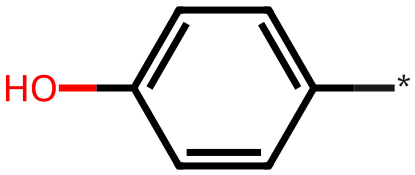
\includegraphics[width=0.9cm,keepaspectratio]{figures/frag_phenol.png} &
% 4.0\ (2.4--6.8) & $2.4\times10^{-5}$ & 4.26\% vs 1.10\% \\[8pt]
% \hline
% \multicolumn{5}{l}{\textit{Complex ring / sugar family}} \\[2pt]
% 2-Methyltetrahydropyran-4-ol &
% \includegraphics[width=0.9cm,keepaspectratio]{figures/frag_methylthp.png} &
% $\infty$\ (6.8, $\infty$) & $1.5\times10^{-4}$ & 1.03\% vs 0\% \\[8pt]
% 4-Amino-2-methyloxan-3-ol &
% \includegraphics[width=0.9cm,keepaspectratio]{figures/frag_aminosugar.png} &
% $\infty$\ (4.3, $\infty$) & $1.7\times10^{-3}$ & 0.74\% vs 0\% \\[8pt]
% Anthracyclinone &
% \includegraphics[width=0.9cm,keepaspectratio]{figures/frag_anthracycline.png} &
% $\infty$\ (4.3, $\infty$) & $1.7\times10^{-3}$ & 0.74\% vs 0\% \\[8pt]
% Methyldecalin &
% \includegraphics[width=0.9cm,keepaspectratio]{figures/frag_methyldecalin.png} &
% 28.4\ (3.4, $\infty$) & $1.7\times10^{-3}$ & 0.88\% vs 0.03\% \\[8pt]
% \hline
% \multicolumn{5}{l}{\textit{Lipophilic chain family}} \\[2pt]
% Ethane &
% \includegraphics[width=0.9cm,keepaspectratio]{figures/frag_ethane.png} &
% 7.2\ (3.0--18.0) & $1.4\times10^{-4}$ & 2.21\% vs 0.31\% \\[8pt]
% Isobutane &
% \includegraphics[width=0.9cm,keepaspectratio]{figures/frag_isobutane.png} &
% 4.8\ (2.4--9.6) & $1.5\times10^{-4}$ & 2.79\% vs 0.59\% \\[8pt]
% Decane &
% \includegraphics[width=0.9cm,keepaspectratio]{figures/frag_decane.png} &
% $\infty$\ (4.3, $\infty$) & $1.7\times10^{-3}$ & 0.74\% vs 0\% \\[8pt]
% \hline
% \multicolumn{5}{l}{\textit{Carbonyl family}} \\[2pt]
% Formaldehyde &
% \includegraphics[width=0.9cm,keepaspectratio]{figures/frag_formaldehyde.png} &
% 5.5\ (2.5--12.2) & $2.1\times10^{-4}$ & 2.35\% vs 0.44\% \\[8pt]
% Methyl ethyl ketone &
% \includegraphics[width=0.9cm,keepaspectratio]{figures/frag_mek.png} &
% $\infty$\ (4.3, $\infty$) & $1.7\times10^{-3}$ & 0.74\% vs 0\% \\[8pt]
% \hline
% \multicolumn{5}{l}{\textit{Halogenated family}} \\[2pt]
% Chloroacetaldehyde &
% \includegraphics[width=0.9cm,keepaspectratio]{figures/frag_chloroacetaldehyde.png} &
% 28.4\ (3.4, $\infty$) & $1.7\times10^{-3}$ & 0.88\% vs 0.03\% \\[8pt]
% \hline
% \multicolumn{5}{l}{\textit{Heteroaromatic family}} \\[2pt]
% Benzimidazole &
% \includegraphics[width=0.9cm,keepaspectratio]{figures/frag_benzimidazole.png} &
% 28.4\ (3.4, $\infty$) & $1.7\times10^{-3}$ & 0.88\% vs 0.03\% \\[8pt]
% \hline
% \end{tabular}
% \end{table*}


% %% ══════════════════════════════════════════════════════════════════════════════
% %% Analysis B — Mito Active vs Inactive (24 frags)
% %% ══════════════════════════════════════════════════════════════════════════════

% % \begin{table*}[h!]
% % \centering
% % \small
% % \caption{%
% %     All 24 BRICS fragments significantly enriched in mitochondrial-active
% %     versus mitochondrial-inactive compounds in HepG2 cells
% %     ($n_{\text{active}} = 972$, $n_{\text{inactive}} = 3{,}196$;
% %     min.\ prevalence $\geq 6$ in active set, OR~$\geq 2$,
% %     Benjamini--Hochberg FDR $\alpha = 0.01$).
% %     OR and 95\,\% CI are conditional maximum-likelihood estimates
% %     (Fisher exact); OR~$= \infty$ with a finite lower bound denotes
% %     fragments absent from the inactive set.
% %     Findings are hypothesis-generating; no external validation set was
% %     used and fragment co-occurrence within molecules is not modelled.
% %     \textit{(Part 1 of 2)}%
% % }
% % \label{tab:brics_mito_enrichment}
% % \begin{tabular}{lp{2.2cm}p{3.0cm}cc}
% % \hline
% % \textbf{Fragment name} &
% % \textbf{Structure} &
% % \textbf{OR (95\,\% CI)} &
% % \textbf{$p_{\text{adj}}$} &
% % \textbf{Prevalence ($n_a$/972 vs $n_i$/3196)} \\
% % \hline

% % \multicolumn{5}{l}{\textit{Phenolic family}} \\[2pt]

% % Para-hydroxyphenyl (phenol) &
% % \includegraphics[width=0.9cm,keepaspectratio]{figures/mi_frag_phenol.png} &
% % 4.6 (2.9--7.4) & $1.7\times10^{-9}$ & 47/972 vs 35/3196 \\[8pt]

% % Pyrogallol (benzene-1,2,3-triol) &
% % \includegraphics[width=0.9cm,keepaspectratio]{figures/mi_frag_pyrogallol.png} &
% % $\infty$ (4.8, $\infty$) & $3.7\times10^{-4}$ & 7/972 vs 0/3196 \\[8pt]

% % Ortho-hydroxyphenyl &
% % \includegraphics[width=0.9cm,keepaspectratio]{figures/mi_frag_ortho_hydroxyphenyl.png} &
% % 3.9 (1.6--9.7) & $3.4\times10^{-3}$ & 13/972 vs 11/3196 \\[8pt]

% % \hline
% % \multicolumn{5}{l}{\textit{Lipophilic chain family}} \\[2pt]

% % \textit{tert}-Butyl (branched C4) &
% % \includegraphics[width=0.9cm,keepaspectratio]{figures/mi_frag_tbutyl.png} &
% % 5.5 (3.0--10.4) & $1.6\times10^{-7}$ & 31/972 vs 19/3196 \\[8pt]

% % Ethylene bridge ($-$CH$_2$CH$_2$$-$) &
% % \includegraphics[width=0.9cm,keepaspectratio]{figures/mi_frag_ethylene.png} &
% % 5.0 (2.1--12.5) & $6.1\times10^{-4}$ & 15/972 vs 10/3196 \\[8pt]

% % Decyl chain (linear C10) &
% % \includegraphics[width=0.9cm,keepaspectratio]{figures/mi_frag_decyl.png} &
% % $\infty$ (3.9, $\infty$) & $1.0\times10^{-3}$ & 6/972 vs 0/3196 \\[8pt]

% % Methylene bridge ($-$CH$_2$$-$, mixed) &
% % \includegraphics[width=0.9cm,keepaspectratio]{figures/mi_frag_methylene_bridge.png} &
% % 2.4 (1.5--3.9) & $1.3\times10^{-3}$ & 32/972 vs 45/3196 \\[8pt]

% % Methine carbon ($-$CH$<$) &
% % \includegraphics[width=0.9cm,keepaspectratio]{figures/mi_frag_methine.png} &
% % 6.1 (2.1--20.1) & $1.4\times10^{-3}$ & 11/972 vs 6/3196 \\[8pt]

% % Decalin/steroid A--B ring &
% % \includegraphics[width=0.9cm,keepaspectratio]{figures/mi_frag_decalin.png} &
% % 19.8 (2.4--913) & $3.1\times10^{-3}$ & 6/972 vs 1/3196 \\[8pt]

% % Octyl chain (linear C8) &
% % \includegraphics[width=0.9cm,keepaspectratio]{figures/mi_frag_octyl.png} &
% % 4.7 (1.6--14.7) & $5.3\times10^{-3}$ & 10/972 vs 7/3196 \\[8pt]

% % gem-Dimethyl (disubstituted) &
% % \includegraphics[width=0.9cm,keepaspectratio]{figures/mi_frag_isobutyl_disub.png} &
% % 6.6 (1.8--30.1) & $5.3\times10^{-3}$ & 8/972 vs 4/3196 \\[8pt]

% % Dodecyl chain (linear C12) &
% % \includegraphics[width=0.9cm,keepaspectratio]{figures/mi_frag_dodecyl.png} &
% % 7.7 (1.8--46.3) & $6.6\times10^{-3}$ & 7/972 vs 3/3196 \\[8pt]

% % Methylene ($-$CH$_2$$-$, sp3) &
% % \includegraphics[width=0.9cm,keepaspectratio]{figures/mi_frag_methylene.png} &
% % 2.1 (1.2--3.6) & $8.3\times10^{-3}$ & 26/972 vs 41/3196 \\[8pt]

% % \hline
% % \end{tabular}
% % \end{table*}


% % \begin{table*}[h!]
% % \centering
% % \small
% % \caption*{\textbf{Table~\ref{tab:brics_mito_enrichment} continued} \textit{(Part 2 of 2)}}
% % \begin{tabular}{lp{2.2cm}p{3.0cm}cc}
% % \hline
% % \textbf{Fragment name} &
% % \textbf{Structure} &
% % \textbf{OR (95\,\% CI)} &
% % \textbf{$p_{\text{adj}}$} &
% % \textbf{Prevalence ($n_a$/972 vs $n_i$/3196)} \\
% % \hline

% % \multicolumn{5}{l}{\textit{Halogenated}} \\[2pt]

% % Trifluoromethyl &
% % \includegraphics[width=0.9cm,keepaspectratio]{figures/mi_frag_cf3.png} &
% % 3.6 (2.0--6.5) & $1.5\times10^{-4}$ & 27/972 vs 25/3196 \\[8pt]

% % Chloroacetyl &
% % \includegraphics[width=0.9cm,keepaspectratio]{figures/mi_frag_chloroacetyl.png} &
% % 23.2 (3.0--1045) & $1.3\times10^{-3}$ & 7/972 vs 1/3196 \\[8pt]

% % Para-chlorophenyl &
% % \includegraphics[width=0.9cm,keepaspectratio]{figures/mi_frag_chlorobenzene.png} &
% % 2.8 (1.5--5.2) & $1.4\times10^{-3}$ & 23/972 vs 27/3196 \\[8pt]

% % \hline
% % \multicolumn{5}{l}{\textit{Nitroaromatic}} \\[2pt]

% % Para-nitrophenyl &
% % \includegraphics[width=0.9cm,keepaspectratio]{figures/mi_frag_nitrophenyl_para.png} &
% % 5.0 (2.1--12.5) & $6.1\times10^{-4}$ & 15/972 vs 10/3196 \\[8pt]

% % \hline
% % \multicolumn{5}{l}{\textit{Carbonyl}} \\[2pt]

% % Disubstituted carbonyl &
% % \includegraphics[width=0.9cm,keepaspectratio]{figures/mi_frag_carbonyl_disub.png} &
% % 4.5 (2.1--9.8) & $3.7\times10^{-4}$ & 19/972 vs 14/3196 \\[8pt]

% % \hline
% % \multicolumn{5}{l}{\textit{Disubstituted aromatic}} \\[2pt]

% % 2-Methyl-1,4-disubstituted phenyl &
% % \includegraphics[width=0.9cm,keepaspectratio]{figures/mi_frag_tolyl_disub.png} &
% % 19.8 (2.4--913) & $3.1\times10^{-3}$ & 6/972 vs 1/3196 \\[8pt]

% % \hline
% % \multicolumn{5}{l}{\textit{Nitrogen-containing}} \\[2pt]

% % Dimethylamine (tertiary amine) &
% % \includegraphics[width=0.9cm,keepaspectratio]{figures/mi_frag_dimethylamine.png} &
% % 7.2 (2.5--23.2) & $3.7\times10^{-4}$ & 13/972 vs 6/3196 \\[8pt]

% % Benzimidazolyl &
% % \includegraphics[width=0.9cm,keepaspectratio]{figures/mi_frag_benzimidazole.png} &
% % 19.8 (2.4--913) & $3.1\times10^{-3}$ & 6/972 vs 1/3196 \\[8pt]

% % Pyridyl (disubstituted) &
% % \includegraphics[width=0.9cm,keepaspectratio]{figures/mi_frag_pyridyl.png} &
% % 9.9 (1.8--101) & $8.0\times10^{-3}$ & 6/972 vs 2/3196 \\[8pt]

% % \hline
% % \multicolumn{5}{l}{\textit{Organophosphate}} \\[2pt]

% % O,O-Dimethyl thiophosphate &
% % \includegraphics[width=0.9cm,keepaspectratio]{figures/mi_frag_dimethylthiophosphate.png} &
% % 23.2 (3.0--1045) & $1.3\times10^{-3}$ & 7/972 vs 1/3196 \\[8pt]

% % \hline
% % \multicolumn{5}{l}{\textit{Deoxysugar / complex ring}} \\[2pt]

% % Methyloxanol (deoxysugar moiety) &
% % \includegraphics[width=0.9cm,keepaspectratio]{figures/mi_frag_methyloxanol.png} &
% % $\infty$ (4.8, $\infty$) & $3.7\times10^{-4}$ & 7/972 vs 0/3196 \\[8pt]

% % \hline
% % \end{tabular}
% % \end{table*}





% % \newpage

% % \rule{0.05in}{1.75in}%
% % \begin{minipage}[b][1.75in]{3.25in}
% %   \sffamily
% %   \frenchspacing

% %   Some journals require a graphical entry for the Table of Contents. This
% %   should be laid out ``print ready'' so that the sizing of the text is correct.

% %   The space available depends on the journal: J. Am. Chem. Soc. allows 3.25 in
% %   by 1.75 in and requires sanserif text. Some journals want different sizes:
% %   you can easily adjust here.
  
% %   The two rules either side of the content are there to help judge the height
% %   of your material: they may be deleted once not required.
  
% % \end{minipage}%
% % \rule{0.05in}{1.75in}

\end{document}
